\documentclass[
pdftex,
a4paper,
oneside,
parskip,
numbers=noenddot,
listof=totoc,
bibliography=totoc,
hyperfootnotes=false
]{scrreprt}
\setuptoc{toc}{totoc}

\newcommand{\thesistitle}{Natürlichsprachliche Mustererkennung für natürlichsprachliche Objektszenarien}
\newcommand{\thesistype}{B A C H E L O R A R B E I T}
\newcommand{\thesistypedesc}{im Fachbereich Elektrotechnik/Informatik \\
der Universität Kassel}
\newcommand{\thesisauthorname}{Adrian Kunz}
\newcommand{\thesisauthorhomestreet}{***REMOVED***}
\newcommand{\thesisauthorhometown}{***REMOVED***}
\newcommand{\thesisauthormatrikelnumber}{35013235}
\newcommand{\thesisauthoremail}{***REMOVED***}
\newcommand{\thesisdepartment}{Fachgebiet Software Engineering}
\newcommand{\thesisfirstreviewer}{Prof.\ Dr.\ Albert Zündorf}
\newcommand{\thesissecondreviewer}{Prof.\ Dr.\ Claude Draude}
\newcommand{\thesissupervisor}{Prof.\ Dr.\ Albert Zündorf}
\newcommand{\thesisdate}{31.\ März 2020}

% geometry
\usepackage[bindingoffset=1cm, left=2.5cm, right=2.5cm, top=2.5cm, bottom=2.5cm]{geometry}

% Headline
\usepackage{fancyhdr}
\pagestyle{fancy}
\renewcommand{\chaptermark}[1]{\markboth{\thechapter\ #1}{}}
\lhead{\leftmark} \rhead{\thepage}
\cfoot{}
\fancypagestyle{plain}{}

% Select input encodung, usually utf8 is the best choice, on windows, \usepackage[latin1]{inputenc} maybe required
\usepackage[utf8]{inputenc}
\usepackage[T1]{fontenc}

% Colors
\usepackage{color}
\usepackage{colortbl}

% Tables
\usepackage{tabularx}
\usepackage{multirow}

% Drawing graphs etc.
\usepackage{pgf}
\usepackage{tikz}
\usetikzlibrary{arrows,automata}

% math
\usepackage{amsmath}

% lists
\usepackage{paralist}

% Figures
\usepackage{graphicx, wrapfig}

% Hyperlinks
\usepackage[hyphens]{url}
\usepackage{hyperref}
\hypersetup{colorlinks, citecolor=black, linkcolor=black, urlcolor=black}

% Minted
\usepackage[chapter]{minted}
%\usemintedstyle{xcode}
\setminted{frame=single,tabsize=2,linenos}

\newmintinline[code]{text}{breaklines}
\newmintinline[mdcode]{md}{breaklines}
\newmintinline[jcode]{java}{breaklines}

\newminted[codeblock]{text}{autogobble,frame=none,linenos=false,breaklines}
\newminted[mdcodeblock]{md}{autogobble,frame=none,linenos=false,breaklines}
\newminted[jcodeblock]{java}{autogobble,frame=none,linenos=false}

\newcommand{\outquote}[1]{``{#1}''}

\newcommand{\codelisting}[4]{%
    \begin{listing}[htp]
        \inputminted{#1}{#2/#3}
        \vspace{-3ex}
        \caption{#4}
        \label{lst:#3}
    \end{listing}%
}

% list of abbreviations
\usepackage[printonlyused]{acronym}

% Set line pitch
\usepackage{setspace}
\onehalfspacing              % anderthalbzeilig (oder auch \doublespace)

% Newcommand TODO (red in text)
\newcommand{\todo}[1]{\textcolor{red}{TODO: #1}}

% Newcommand TODOM (red at border)
\newcommand{\todom}[1]{\marginpar{\parbox{1.5cm}{\textcolor{red}{TODO:\\ #1}}}}

%fancyBox
%\usepackage{fancybox}

% Layout corrections (Schusterjungen)
\clubpenalty = 10000
% Layout corrections (Hurenkinder) 
\widowpenalty = 10000
\displaywidowpenalty = 10000

% Figures
\usepackage{caption}
\usepackage[hypcap=true,labelformat=simple]{subcaption}
\renewcommand{\thesubfigure}{(\alph{subfigure})}

% Tables
\usepackage{booktabs}

% Frequently used column types
\newcolumntype{C}[1]{>{\centering\arraybackslash}p{#1}} % centering column type with fixed width
\newcolumntype{R}[1]{>{\raggedleft\arraybackslash}p{#1}} % right aligned column type with fixed width
\newcolumntype{L}[1]{>{\raggedright\arraybackslash}p{#1}} % left aligned column type with fixed width

% Shortcuts for referencing floats:
\newcommand{\fig}[1]{\figurename~\ref{#1}} %shortcut for a figure reference
\newcommand{\tab}[1]{Table~\ref{#1}} %shortcut for a table reference
\newcommand{\eq}[1]{(\ref{#1})} %shortcut for an equation reference
\newcommand{\lst}[1]{Listing~\ref{#1}} %shortcut for a listing reference
\newcommand{\sect}[1]{Section~\ref{#1}} %shortcut for a Section reference


\usepackage[ngerman]{babel}

\begin{document}

	\pagenumbering{roman}

	\begin{titlepage}
	%select font without serifs
	\sffamily

	% Logo
	\begin{tabularx}{\textwidth}{@{}l@{}>{\raggedleft\arraybackslash}X@{}r@{}}
		\multirow{2}{*}{
\includegraphics[width=6.8cm]{images/Logo_UniKassel}} &
		\raisebox{-1mm}{\small{Fachbereich Elektrotechnik/Informatik}} \\
		&\raisebox{-1mm}{\small{\thesisdepartment}} &
	\end{tabularx}

	\vspace{2.5cm}

	\begin{center}
		% Title and subtitle
		\huge{\thesistitle}

		\vspace{3cm}

		\renewcommand{\baselinestretch}{1.3}
		\Large{\thesistype}

		\large
		\thesistypedesc
	\end{center}

	\vspace{1.5cm}
	\renewcommand{\baselinestretch}{1}
	\begin{table}[htpb]
		\centering
		\begin{tabular}{ll}
			\\
			Eingereicht von: & \thesisauthorname \\
			Anschrift: & \thesisauthorhomestreet \\
			& \thesisauthorhometown \\
			\\
			Matrikelnummer: & \thesisauthormatrikelnumber \\
			E-Mail: & \thesisauthoremail \\
			\\
			Vorgelegt im: & \thesisdepartment \\
			\\
			Erstprüfer: & \thesisfirstreviewer \\
			Zweitprüferin: & \thesissecondreviewer \\
			\\
			Betreuer: & \thesissupervisor \\
			\\
			Eingereicht am: & \thesisdate \\
		\end{tabular}
	\end{table}

	% font with serifs
	\rmfamily
\end{titlepage}

	\chapter*{Zusammenfassung}

% Inhaltsverzeichnis und Kopfzeile
\addcontentsline{toc}{chapter}{Zusammenfassung}
\markboth{Zusammenfassung}{Zusammenfassung}

Diese Arbeit führt eine neue Online-Plattform für elektronische Lehre ein, die thematisch auf Datenmodellierung fokussiert ist.
Dafür wird eine neue Beschreibungssprache vorgestellt, die die Modellierung anhang von textuellen Beispielszenarien in natürlicher Sprache ermöglicht.
Auf der Online-Plattform ist das Einreichen von Aufgaben und Lösungen möglich, wovon letztere automatisch korrigiert werden können.
Dies wird durch Funktionalität zur Mustererkennung auf beliebigen Objektstrukturen in der Sprache der Beispielszenarien realisiert.


	\tableofcontents

	\pagebreak
	\pagenumbering{arabic}
	\addtocontents{toc}{\protect\vspace{1.0cm}}

	\chapter{Einleitung / Introduction}

Some guidelines and examples are given in the following.

\section{Citations}

Citations should be made using BibTeX in the file \verb|thesis.bib|.
Using BibTeX, different styles are available for different types of publications. Examples are books \cite{Adams90}, journal articles \cite{Zhang99}, conference proceeding \cite{Yee99} and
electronic resources \cite{Fear05}. Multiple references can be made by \cite{Adams90,Zhang99,Yee99,Fear05}.


\section{Figures}

A simple example of a figure can be found in \fig{fig:simple_figure}. A more complex figure including subfigures is show in \fig{fig:figure_with_subfigures}. Here each subfigure can be addressed separately (e.g., \fig{fig:subfigure1} and \fig{fig:subfigure2}). Please use vector graphics (pdf, eps obtained from svg, etc.) whenever possible. Pixel formats like jpeg, bmp, etc. should only be used for real photographs.

\begin{figure}[!h]
	\centering
	\fbox{\parbox{5cm}{\centering ~\vspace{1.5cm}\\Dummy\\~\vspace{1.5cm}}} %replace this line by: \includegraphics{path to image}
	\caption{Simple figure}
	\label{fig:simple_figure}
\end{figure}

\begin{figure}[!h]
	\centering
	\begin{subfigure}[b]{7cm}
		\centering
		\fbox{\parbox{5cm}{\centering ~\vspace{1.5cm}\\Dummy\\~\vspace{1.5cm}}} %replace this line by: \includegraphics{path to image}
		\caption{Caption of subfigure a (can be empty)}
		\label{fig:subfigure1}
	\end{subfigure}
	\begin{subfigure}[b]{7cm}
		\centering
		\fbox{\parbox{5cm}{\centering ~\vspace{1.5cm}\\Dummy\\~\vspace{1.5cm}}} %replace this line by: \includegraphics{path to image}
		\caption{Caption of subfigure b (can be empty)}
		\label{fig:subfigure2}
	\end{subfigure}
	\caption{Figure using subfigures}
	\label{fig:figure_with_subfigures}
\end{figure}


\section{Tables}

Examples of tables can be found in \tab{tab:simple_table} and \tab{tab:complex_table}. In general vertical lines are not necessary and should be avoided (see \cite{Fear05} for more about table styles).

\begin{table}[!h]
	\renewcommand{\arraystretch}{1.1}
	\caption{A very simple table}
	\label{tab:simple_table}
	\centering
	\begin{tabular}{cccc}
		\toprule
		& Apple & Orange & Banana \\
		\midrule
		Colour       & green & orange & yellow\\
		\bottomrule
	\end{tabular}
\end{table}

\begin{table}[!h]
	\renewcommand{\arraystretch}{1.1}
	\caption{An example of a more complex table}
	\label{tab:complex_table}
	\centering
	\begin{tabular}{ccC{1cm}C{1cm}C{1cm}C{1cm}C{1cm}C{1cm}C{1cm}C{1cm}C{1cm}C{1cm}C{1cm}}
		\toprule
		& & \multicolumn{4}{c}{RPAG algorithm} & \multicolumn{5}{c}{RPAGT (proposed)}\\
		\cmidrule(rl){3-6} \cmidrule(rl){7-11}
		$N$ & $N_\text{uq}$ & S & add ops & pure reg. & reg. ops & S & add ops & pure reg. & reg. ops & impr.\\
		\cmidrule(rl){1-11}
		6   & 3  & 3 & 8  & 1 & 9  & 2 & 5  & 0 & 5  & 44.4\% \\
		10  & 5  & 3 & 10 & 3 & 13 & 2 & 6  & 2 & 8  & 38.5\% \\
		13  & 7  & 3 & 14 & 2 & 16 & 2 & 8  & 2 & 10 & 37.5\% \\
		20  & 10 & 3 & 15 & 4 & 18 & 2 & 9  & 3 & 12 & 33.3\% \\
		28  & 14 & 3 & 20 & 3 & 23 & 2 & 15 & 2 & 17 & 26.1\% \\
		41  & 21 & 3 & 31 & 1 & 32 & 2 & 23 & 2 & 25 & 21.9\% \\
		61  & 31 & 3 & 39 & 3 & 42 & 2 & 32 & 2 & 34 & 19.0\% \\
		119 & 54 & 3 & 62 & 7 & 69 & 2 & 56 & 1 & 57 & 17.4\% \\
		151 & 71 & 3 & 79 & 4 & 83 & 2 & 72 & 2 & 74 & 10.8\% \\
		\cmidrule(rl){1-11}
		avg.: & 24 & & 30.89 & 3.56 & 33.89 & & 25.11 & 1.78 & 26.89 & 27.7\% \\
		\bottomrule
	\end{tabular}
\end{table}

\section{Listings}

Listings can be included in the text using the \verb|lstlisting| environment. An example listing is shown in \lst{lst:pseudocode}. The listing format is set for pseudocodes (based on the C language). For other languages adjust the settings in \verb|header.tex|.

\begin{lstlisting}[float,caption=RPAGT Algorithm,label=lst:pseudocode]
	RPAGT($T$)
	$\displaystyle S := \max_{t\in T} \, \text{AD}_{\text{min}}^3(t)$
	$X_S := \{\text{odd}(t) \ | \ t \in T\} \setminus \{0\}$
	for $s=S\ldots 2$
	$W := X_s$
	$P := \emptyset$
	do
	$p \leftarrow \text{best\_single\_predecessor}(P,W,s)$
	if $p \neq 0$
	$P \leftarrow P \cup \{p\}$
	else
	$P' \leftarrow \text{best\_msd\_predecessor\_set}(W,s)$
	$P \leftarrow P \cup P'$
	$W \leftarrow W \setminus \mathcal{A}^3_{*}(P)$
	while $|W|\neq \emptyset$
	$X_{s-1} \leftarrow P$
\end{lstlisting}

\section{ToDo's}

During the writing of the thesis, ToDo's in the text can be highlighted using \verb|\todo|. Notes at the border of the text can be done using \verb|\todom|.
\todo{This has to be more extended}
\todom{ToDo remark at the border}

	\chapter{Zielsetzung}\label{ch:goals}

Auf hoher Ebene ist das Ziel dieser Arbeit, die Grundlage für eine E-Learning-Platform zu schaffen.
Diese soll zunächst auf das Thema der Datenmodellierung beschränkt sein, aber konzeptuell die Erweiterung auf andere Themengebiete auch außerhalb der Informatik erlauben.
Es soll möglich sein, Aufgaben bei dieser Platform einzureichen, die von Studierenden oder anderen Interessengruppen bearbeitet werden können.
Der Ersteller der Aufgabenstellung soll in der Lage sein, deren Anforderungen so zu spezifizieren, dass Lösungen automatisch bewertet werden können.
Die automatische Bewertung soll nicht nur nach Abgabe sondern auch während der Bearbeitung durchgeführt werden, um sofortiges Feedback zu ermöglichen.
Nach dem Einreichen von Lösungen sollen diese für Ersteller der Aufgabenstellung und erwählte weitere Personen zugänglich sein, um die automatische Bewertung bei Bedarf durch eine händische zu ergänzen.
Dies ist explizit optional, um die Bereitstellung von unbeaufsichtigten, öffentlich zugänglichen Aufgaben in Form von interaktive Tutorials zu ermöglichen.
Eine Erweiterung des Aufgabenkonzepts sieht vor, diese in Gruppen oder ganze Kurse zusammenfassen zu können.
Deren Ziel ist es, das Konzept auf größere Themengebiete übersichtlich auszuweiten.

Speziell im Kontext der Modellierung gilt es, gewisse Freiheiten in Lösungen von Aufgaben zu erlauben.
Dazu gehört besonders die Freiheit der Namensgebung, sofern diese nicht explizit vorgegeben ist.
Bei konkreten Modellierungsaufgaben soll jedoch auch die Verwendung von abweichenden Werten gestattet sein.
Der Aufgabenersteller soll in der Lage sein, nach eigenem Ermessen Anforderungen und Toleranzbereiche festzulegen.
Dies soll seitens des Lernenden den Fokus auf konzeptuelle Hintergründe der Modellierung ermöglichen, indem beispielspezifische Details weniger Bedeutung erhalten.

	\chapter{Stand der Technik}\label{ch:state-of-the-art}

\todo{
EMF (Eclipse Modeling Framework) ???,
SDMLib (Story-Driven Modeling Library)~\cite{networkparser},
}

	\chapter{Fulib Scenarios}\label{ch:fulib-scenarios}

Dieses Kapitel befasst sich mit dem natürlichsprachlichen Aspekt dieser Arbeit.
Es betrachtet das Fulib Scenarios Projekt, das in Vorbereitung auf die weiteren Inhalte entstanden ist.
Dessen Ziel war es, eine Beschreibungssprache für Objektstrukturen und Abläufe zu entwickeln.
Diese Abläufe werden Scenarios genannt und sind mit User Stories gleichzusetzen.
Sie ermöglichen dabei eine einfache Form der Dokumentation.
Die Verständlichkeit soll sowohl für Entwickler als auch für Personen mit nicht-technischem Hintergrund gewährleistet werden.
Dabei sollen Entwickler unter Beaufsichtigung und Beratung mit Domänenexperten Scenarios erstellen können, um die Anforderungen von Software zu erarbeiten.
Dieser Vorgang wurde bereits in~\cite{explain} erforscht.

Scenarios haben als Werkzeug sowohl in der Modellierung als auch beim Testen eine Bedeutung.
Einerseits lassen sich aus diesen mit vergleichsweise geringem Aufwand umfangreiche Datenmodelle erzeugen, aus denen automatisch Code generiert werden kann.
Sie erfüllen damit eine ähnliche Funktion wie das Eclipse Modeling Framework~\cite{emf} (EMF) oder das als Vorgänger entstandene SDMLib~\cite{networkparser}-Framework.
Der zugrundeliegende Ansatz beim Erstellen von Datenmodellen mit Fulib Scenarios unterscheidet sich jedoch stark von diesen.
Während das EMF auf graphische Werkzeuge setzt, wird in SDMLib das Datenmodell mit imperativem Java-Code definiert.
Fulib Scenarios hingegen setzt auf eine textuelle Beschreibung konkreter Objekte, aus der das Datenmodell abgeleitet wird.
Vorteil davon ist, dass aufgrund des konkreten Ablaufs automatisch ein Test abgeleitet werden kann.
Dieser kann auch nach Änderungen an der Software sicherstellen, dass die ursprüngliche, vom Scenario beschriebene User Story noch gültig und durchführbar ist.

Der folgende Abschnitt befasst sich zunächst mit den Grundlagen von Scenarios.
Daraufhin wird anhand eines Beispiels erklärt, wie ein Scenario verarbeitet wird, um daraus ein Datenmodell und Tests zu generieren.

\section{Sprache}\label{sec:language}

Kern dieser Arbeit ist eine neue Programmiersprache für textuelle Beispielszenarien.
Diese trägt den Namen Scenario-Sprache.
Ziel der Scenario-Sprache ist es, verständlich für jeden zu sein, der Englisch spricht.
Um als Programmiersprache funktionsfähig zu sein, hat sie im Gegensatz zu Englisch eine feste und eingeschränkte grammatikalische Struktur.
Somit handelt es sich um eine Untermenge der Englischen Sprache.
Des Weiteren basiert die Scenario-Sprache auf dem Markdown-Format,
das es erlaubt, einfachen Text mit Überschriften, Fett- und Kursivschreibung, Bildern u.ä.\ zu versehen.
Markdown-Dateien können leicht in HTML umgewandelt werden.
Somit können in der Scenario-Sprache verfasste Dateien als Dokumentation verwendet werden.
Im Folgenden werden einige Grundlagen der Scenario-Sprache dargestellt und erklärt.

\subsection{Grundlagen}\label{subsec:basics}

In der Scenario-Sprache verfasster Quellcode wird in \code{.md}-Dateien abgelegt.
Diese beginnen stets mit einer Überschrift, welche in Markdown mit dem \mdcode{#}-Symbol beginnen.
Mit der Überschrift beginnt ein \emph{Scenario};
deren Text wird zu dessen Namen.
Eine Scenario-Datei kann mehrere Überschriften und damit mehrere Scenarios enthalten.

Nach einer Überschrift können ein oder mehrere Sätze und Unterüberschriften folgen;
diese Bilden den Rumpf des Scenarios.
Unterüberschriften sind an \mdcode{##} am Anfang einer Zeile zu erkennen und ermöglichen die Strukturierung von langen Scenarios.

Im Rumpf von Scenarios gibt es einige Möglichkeiten, Kommentare zu hinterlassen.
Mit \jcode{//} wird wie in anderen Programmiersprachen ein Zeilenkommentar begonnen,
der mit dem nächsten Zeilenumbruch endet.
Dieser ist sowohl nach Umwaldeln des Markdown in HTML sichtbar,
als auch im erzeugten Java-Quellcode vorhanden.
Text der in runden Klammern \code{(...)} steht ist ebenfalls im HTML sichtbar,
jedoch nicht im Java-Quellcode.
Zuletzt können mit \mdcode{<!-- ... -->} Kommentare eingebettet werden,
die weder im HTML sichtbar noch im Java-Code vorhanden sind.

\subsection{Einfache Sätze und Ausdrücke}\label{subsec:simple-sentences-and-expressions}

Sätze bilden den Inhalt eines Scenarios und definieren dessen Ablauf.
Die Scenario-Sprache definiert eine Vielzahl von Sätzen,
die sich sowohl in ihrer Funktionalität ergänzen,
als auch syntaktische Alternativen mit gleicher Semantik füreinander darstellen.

Die einfachste Art von Satz ist der \code{Is}-Satz.
Dieser ermöglicht es, ein Objekt zu definieren und diesem Name und Typ zuzuweisen.
Ein Beispiel dafür ist

\code{Kassel is a City.}

Dabei ist \code{Kassel} der Name des Objekts,
und \code{City} dessen Typ.
\code{is} und \code{a} sind Schlüsselwörter.
Die äquivalente Java-Anweisung ist

\jcode{City kassel = new City();}

Zu beachten ist hier, dass die Klasse \code{City} nicht vorher deklariert werden muss.
Durch Verwenden des Namens wird diese automatisch angelegt.
Es gibt in der Scenario-Sprache keine Syntax für das manuelle Definieren von Klassen.

Ein weiterer einfacher Satz ist der \code{Has}-Satz.
Damit können Attribute von bereits bestehenden Objekten einen Wert zugewiesen bekommen.
Ein Beispiel dafür ist folgendes:

\code{Kassel has postcode 34117.}

Dabei ist \code{Kassel} der Name des Zielobjekts, in diesem Fall jenes, welches zuvor mit dem \code{Is}-Satz angelegt wurde.
\code{postcode} ist der Name des Attributs; \code{34117} der zuzuweisende Wert.
Aus diesem Satz wird der folgende Java-Code:

\jcode{kassel.setPostcode(34117)}

Wieder ist zu beachten, dass das Attribute \code{postcode} bzw.\ der Setter \code{setPostcode} nicht im Vorhinein deklariert wurde;
dieses wurde durch die Verwendung automatisch angelegt.
Durch den Ausdruck \code{34117} konnte ermittelt werden, dass der Typ dieses Attributes \code{int} sein muss.
Wäre der Wert stattdessen \code{D-34117}, was von der Scenario-Sprache als Zeichenkette verstanden wird,
hätte das Attribut den Typ \code{String} erhalten und der entsprechende Java-Code wäre \jcode{kassel.setPostcode("D-34117")}.

Da das Definieren von Objekten und die Zuweisung von Attributen sehr häufig in Kombination geschieht, bietet die Scenario-Sprache eine alternativ Satzart an, die beides gleichzeitig durchführt.
Diese Sätze heißen \code{There}-Sätze.
Die obigen Beispiele lassen sich mit einem There-Satz verkürzen:

\code{There is the City Kassel with postcode 34117.}

Hierbei sind die Schlüsselwörter \code{There is the} der Ersatz für \code{is},
während \code{has} durch \code{with} ersetzt wurde.
Der Java-Code ist äquivalent zu den beiden zuvor gezeigten Zeilen.

Bei erneuter Betrachtung des Java-Codes fällt auf, dass das Wort \code{Kassel} darin nur als Variablenname, jedoch nicht als Wert vorkommt.
Somit ist der Name der Stadt zur Laufzeit nicht zu ermitteln;
dies ist bei der Modellierung von Objektstrukturen i.d.R.\ unpraktisch.
Aus diesem Grund bieten \code{There}-Sätze eine Möglichkeit, eine Zeichenkette sowohl als Attributwert als auch als Variablennamen zu verwenden:

\code{There is a City with name Kassel and with postcode 34117.}

Hier ist zu sehen, dass in einem \code{There}-Satz mehrere Attributzuweisungen mit \code{with} möglich sind, indem sie durch \code{and} getrennt werden\footnote{
Alternativ können diese auch durch \code{,} (Komma) und \code{, and} (And mit Oxford-Komma) getrennt werden, da dies bei mehr als zwei \code{with} die Lesbarkeit erhöht.
}.
Das ansonsten unbenannte Objekt bezieht seinen Namen aus der ersten Attributzuweisung,
heißt also wieder \code{kassel}.
Der entsprechende Java-Code ist wie folgt:

\jcode{City kassel = new City();}\\
\jcode{kassel.setName("Kassel");}\\
\jcode{kassel.setPostcode(34117);}

Als nächstes soll die \code{City}-Klasse eine Assoziation erhalten.
Dafür wird zunächst ein anderes Objekt, hier \code{germany}, und eine andere Klasse, hier \code{Country}, benötigt.
Eine Assoziation von \code{kassel} zu \code{germany} kann nun wie ein Attribut angelegt werden.

\code{There is a country with name Germany.}\\
\code{Kassel has country Germany.}

Der entsprechende Java-Code ist:

\jcode{Country germany = new Country();}\\
\jcode{germany.setName("Germany");}\\
\jcode{kassel.setCountry(germany);}

Nun ist \code{country} eine \emph{unidirektionale} Zu-1-Assoziation von \code{City} zu \code{Country}.
Um diese bidirektional zu machen, muss der Name sowie die Kardinalität der Rückrichtung angegeben werden:

\code{Kassel has country and is one of the cities of Germany.}

Dabei ist \code{cities} der Name der Rückrichtung.
Die zugehörige Java-Zeile ist wie zuvor \jcode{kassel.setCountry(germany);}.
Offensichtlich ist der Name der Rückrichtung nicht in dieser vertreten.
Lediglich anhand des Quellcodes der \code{City}- bzw. \code{Country}-Klassen lässt sich dieser Zusammenhang erschließen.
\code{one of} gibt an, dass es sich dabei um eine Zu-n-Assoziation handelt;
durch dessen Entfernen kann auch die Rückrichtung zu-1 gemacht werden.
Dies ist aber in diesem Beispiel unerwünscht, da ein Land mehr als eine Stadt haben kann.

Alternativ kann die Assoziation auch ausgehend vom \code{Germany}-Objekt definiert werden:

\code{Germany has cities and is the country of Kassel and Berlin.}

Wichtig ist dabei, dass mehrere Zielobjekte angegeben werden (\code{Kassel} und \code{Berlin}, davon ausgehend dass \code{Berlin} analog zu \code{Kassel} definiert wurde).
Andernfalls würde aus \code{cities} trotz der Pluralform eine Zu-1-Assoziation werden.

\subsection{Test-Sätze und Diagramme}\label{subsec:test-sentences-and-diagrams}

Während die erzeugten Klassen Teil zum Programmquellcode gehören,
werden aus den Sätzen eines Scenarios Tests generiert.
Genauer wird aus jeder Scenario-Datei eine Testklasse,
und aus jedem Scenario wird eine Testmethode.
Mit Ausnahme von Sätzen, die zu Aufrufen gehören (siehe Unterabschnitt~\ref{subsec:methods}),
werden aus jedem Satz eine oder mehrere Anweisungen im Rumpf dieser Testmethode.

Damit Tests aussagekräftig sind, müssen sie die Ergebnisse der durchgeführten Aktionen überprüfen.
Dazu dienen in Java Assertions, welche sowohl von der Sprache als Schlüsselwort als auch von verschiedenen Test-Frameworks bereitgestellt werden.
Die Scenario-Sprache generiert Test-Code, der das Test-Framework JUnit~4~\cite{junit4} verwendet.
Sie bietet einige Sätze an, die auf Assertions abgebildet werden;
diese werden zusammengefasst als \code{Expect}-Sätze bezeichnet.
Im Folgenden werden diese nur in einer einfachen, statischen Form betrachtet.
Kapitel~\ref{ch:pattern-matching} führt eine erweiterte Form ein, die dynamische Erwartungen an Objektstrukturen mithilfe von Mustererkennung ermöglicht.

\code{Expect}-Sätze sind zu erkennen an dem Schlüsselwort \code{expect}, dem das Schlüsselwort \code{We} vorangestellt ist.
Diese stellt den Handelnden des Satzes da, wobei sich ``Wir'' auf den Test bezieht.
Bestimmte Sätze erlauben andere Handelnde;
dies wird in Unterabschnitt~\ref{subsec:methods} behandelt.
Ein Beispiel für einen \code{Expect}-Satz auf dem im vorherigen Unterabschnitt erstellten Objekt \code{kassel} ist:

\code{We expect that Kassel has postcode 34117.}

Dieser Satz fragt den Wert des \code{postcode}-Attributs des \code{kassel}-Objekts ab, und prüft ob dieser gleich 34117 ist.
Zu beachten ist hierbei die Analogie zu dem \code{has}-Satz, der in vorherigen Unterabschnitt das Attribut des \code{kassel}-Objekts gesetzt hat.
Der Satz erzeugt die folgende Java-Anweisung:

\jcode{assertEquals(34117, kassel.getPostcode())}

Der gleiche Java-Code wird generiert, wenn man den Satz umstellt:

\code{We expect that postcode of Kassel is 34117.}

Dabei ist \code{of} ein Schlüsselwort, mit dem der Wert eines Attributs erhalten werden kann.
Das Schlüsselwort \code{is} dient hier als binärer Operator der Gleichheit.
Würde man \code{34117} und \code{postcode of Kassel} vertauschen, würde der resultierende Satz die gleiche Bedeutung haben,
mit dem Unterschied dass Erwartungs- und tatsächlicher Wert der Assertion getauscht wären.
Neben \code{is} existieren weitere Operatoren zum Vergleichen von Werten;
diese werden in Unterabschnitt~\ref{subsec:control-structures} näher erläutert.

Die Scenario-Sprache bietet neben automatischen Tests auch die Möglichkeit, Objektstrukturen zu visualisieren.
Diese können sowohl der Verständlichkeit dienen als auch für die Dokumentation verwendet werden.
Dafür kommen Diagrammsätze zum Einsatz, die die Markdown-Syntax für Bilder (\mdcode{![Beschreibung](dateiname.png)}) verwenden und daher keine englischen Sätze sind.
Als Beschreibung dienen ein oder mehrere Objekte, die mit ihren über Assoziationen erreichbaren Nachbarn in einem Objektdiagramm dargestellt werden.
Dafür wird die FulibTools\cite{fulibTools}-Bibliothek verwendet.
Diese kann gegeben einige Startobjekte einen Objektgraphen bilden, diesen übersichtlich anordnen und als PNG-Bild oder Vektorgrafik zeichnen.
Um die zuvor definierten und verknüpften Objekte darzustellen, kann der folgende Diagramm-Satz verwendet werden:

\mdcode{![Germany](germany.png)}

Dies entspricht dem Aufruf zur Verwendung von FulibTools:

\jcode{FulibTools.objectDiagrams().dumpPng("germany.png", germany);}

Führt man das Scenario aus, wird die Datei \code{germany.png} erstellt.
Abbildung~\ref{fig:germany.png} zeigt das Objektdiagramm, das von dieser darstellt wird.

\begin{figure}
    \centering
    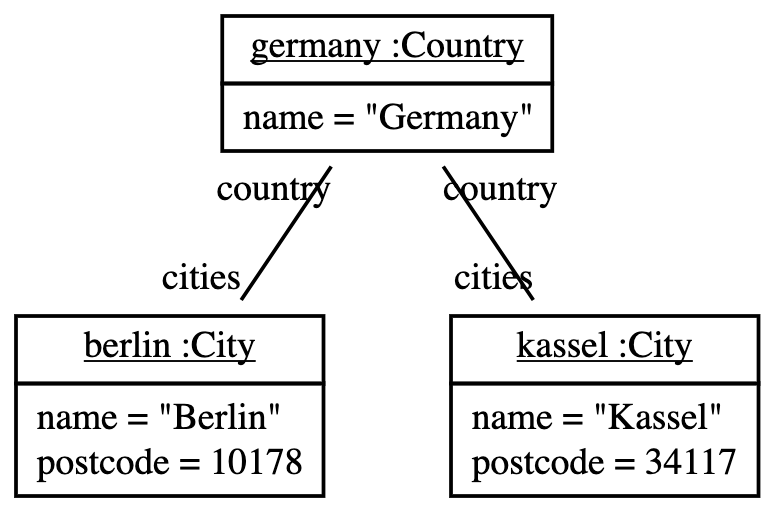
\includegraphics[width=0.5\textwidth]{chapter/fulib-scenarios/img/germany.png}
    \caption{Objektdiagramm von \code{germany}}
    \label{fig:germany.png}
\end{figure}

Neben der Dateiendung \code{.png} wird auch \code{.svg} für Vektorgrafiken unterstützt.
Diese werden zwar vergrößert besser dargestellt, eignen sich aber u.U.\ nicht für die Einbettung in Markdown.
Des Weiteren existieren diverse weitere Ausgabeformate, welche in der Dokumentation~\cite[Language.Sentences.Test Sentences.Diagram Sentences]{documentation} näher erläutert werden.

\subsection{Kontrollstrukturen}\label{subsec:control-structures}

Mit Scenarios lassen sich nicht nur statische Objektstrukturen erzeugen.
Es ist auch möglich, zur Laufzeit Entscheidungen zu fällen und davon abhängig unterschiedliche Ergebnisse zu erzeugen.
Dafür kommen \code{As}-Sätze zum Einsatz.
Diese entsprechen If-Anweisungen in Java, jedoch mit dem konzeptuellen Unterschied,
dass im Scenario vom Eintreten der Bedingung ausgegangen wird.
Daraus folgt die Verwendung des Schlüsselworts \code{As} statt \code{If},
sowohl die fehlende Syntax für \code{else}-Zweige\footnote{
Dies lässt sich durch Verwenden von zwei \code{As}-Sätzen mit gegensätzlichen Bedingungen umgehen.
}.

Das folgende Beispiel soll zur Illustration dieser Sätze dienen:

\code{As semester of Alice is less than 3, we add Maths to courses of Alice.}

Der \code{As}-Satz nimmt hier die Form \code{As <condition>, <sentence>.} an.
In der Bedingung wird der Wert des Attributs \code{semester} des Objekts \code{Alice} mit \code{3} verglichen, wobei \code{is less than} gleichzusetzen ist mit \code{<}.
Die Scenario-Sprache definiert Operatoren für Gleichheit (\code{is}), Ungleichheit (\code{is not}), Größer/Kleiner Als (\code{is greater/less than}) und Größer/Kleiner Gleich (\code{is greater/less equal}).

Ist die Bedingung wahr, wird der nachstehende Satz ausgeführt.
In diesem Beispiel ist dies ein \code{Add}-Satz, der Zahlen addieren und Elemente zu Listen bzw.\ Zu-n-Assoziationen hinzufügen kann.
In diesem Fall sind \code{Maths} und \code{Alice} im Vorhinein deklarierte Objekte;
\code{courses} ist eine Zu-n-Assoziation von der Klasse von \code{Alice} zu der Klasse von \code{Maths}.

Der zum obigen Beispiel gehörende Java-Code ist:

\jcode|if (alice.getSemester() < 3) {|\\
\jcode|    alice.withCourses(maths);|\\
\jcode|}|

Um mehrere Sätze im Rumpf der If-Anweisung zu erhalten, können mehrere Sätze hinter dem \code{As}-Satz durch \code{and} getrennt werden:

\code{As Alice has done Maths, we add 6 to credits of Alice and we remove 3 from motivation of Alice.}

\jcode|if (alice.getDone().contains(maths)) {|\\
\jcode|   alice.setCredits(alice.getCredits() + 6);|\\
\jcode|   alice.setMotivation(alice.getMotivation() - 3);|\\
\jcode|}|

Die zweite Art von Kontrollstruktur in der Scenario-Sprache ist der \code{Take}-Satz, der auf \code{for}-Schleifen in Java abgebildet wird.
Dieser nimmt die Form \code{We take a <name> from <expr> and <sentence...>} an, wobei \code{<name>} den Namen der Schleifenvariable, \code{<expr>} die zu durchlaufende Liste und \code{<sentence...>} den Schleifenrumpf bilden.
Im folgenden Beispiel ist diese Form ersichtlich:

\code{We take a student from students of uni and we add 1 to semester of student.}

Übersetzt in Java-Code ergibt sich die \code{for}-Schleife:

\jcode|for (Student student : uni.getStudents()) {|\\
\jcode|    student.setSemester(student.getSemester() + 1);|\\
\jcode|}|

Wichtig bei der Verwendung von \code{take} ist, dass der Ausdruck nach \code{from} einen \emph{Listentyp} hat.
Diese entsprechen in Java dem Typ \jcode{java.util.List<T>}, wobei \code{T} der Elementtyp ist.
Der Getter von Zu-n-Assoziationen hat automatisch einen Listentyp mit der Zielklasse als Elementtyp.

Es ist jedoch auch möglich, Listenausdrücke zu verwenden.
Diese bestehen in der einfachsten Form aus anderen Ausdrücken, die durch Komma oder \code{and} getrennt sind.
Beispiele dafür sind \code{1, 2, 3}, \code{Alice, Bob and Charlie} und \code{'left' and 'right'}.
In Java werden daraus Ausdrücke wie \code{Arrays.asList(1, 2, 3)} vom Typ \code{List<Integer>}.

Diese Listen lassen sich beispielsweise mit \code{write}-Sätzen in einer Variable speichern:

\code{We write Alice, Bob and Charlie into students.}

Daraus entsteht der folgende Java-Code:

\jcode{List<Student> students = new ArrayList<>(Arrays.asList(alice, bob, charlie));}

Zu beachten ist hier die Verwendung von \code{ArrayList};
durch diese können der Liste Elemente hinzugefügt oder entfernt werden.
Dies ist mit den \code{add}- und \code{remove}-Schlüsselwörtern möglich:

\code{We add David to students.}\\
\code{We remove Bob and Charlie from students.}

\jcode{students.add(david);}\\
\jcode{students.removeAll(bob, charlie);}

\todo{
Ranges?,
Vector Access?,
Contains conditional operator?,
Filter?,
}

\subsection{Methoden}\label{subsec:methods}

\todo{
Aufrufe,
Handelnde,
Stückweise Definition,
}

\todo{
The paper~\cite{explain}.
}

\section{Compiler}\label{sec:compiler}

Damit eine Programmiersprache verwendbar ist, muss sie nicht nur eine Spezifikation haben, sondern auch ausführbar sein.
Dies kann durch direktes Ausführen des Programmtexts geschehen;
in diesem Fall wird das ausführende Programm Interpreter genannt.
Andererseits kann eine Programmiersprache auch in ein maschinenlesbares Format übersetzt werden,
das dann direkt oder durch eine virtuelle Maschine ausgeführt wird.
Dieser Ansatz nennt sich Kompilierung.
In Java wird die Kompilierung durch den Java Compiler (\code{javac}) durchgeführt, welcher Bytecode erzeugt;
dieser kann von einer Java Virtual Machine (JVM) ausgeführt werden.

FulibScenarios wird hingegen in zwei Schritten kompiliert.
Zunächst werden die Markdown-Scenario-Quelltexte in Java-Quelltexte übersetzt;
dies ist Aufgabe des Scenario-Compilers.
Der erzeugte Java-Quellcode wird dann vom Java-Compiler kompiliert.
Die Architektur und Implementierung des Scenario-Compilers sind Inhalt dieses Abschnitts.
Dabei wird des öfteren auf das Beispiel in Listing~\ref{lst:CompilationExample.md} Bezug genommen,
dessen Übersetzung bis zum Java-Quellcode in den einzelnen Teilabschnitten stückweise erarbeitet wird.

\begin{listing}[htp]
    \centering
    \code{src/main/scenarios/org/example/CompilationExample.md}
    \inputminted{md}{chapter/fulib-scenarios/scenarios/CompilationExample.md}
    \vspace{-3ex}
    \caption{Beispiel-Szenario zur Demonstration des Scenario-Compilers}
    \label{lst:CompilationExample.md}
\end{listing}

\subsection{Architektur}\label{subsec:compiler-architecture}

Die Kompilierung von Programmiersprachen ist eine komplexe Aufgabe,
bei der viele Schritte zum Ergebnis beitragen und zusammenwirken müssen.
Deshalb ist es wichtig, dass ein Compiler diese in einer übersichtlichen Architektur aufbaut.
Diese Schritte werden auch als \emph{Phasen}\cite[4]{dragonbook} bezeichnet.
Im Groben kann der Scenario-Compiler in drei Schritte unterteilt werden,
deren Aufgaben sich stark unterscheiden.

Die erste Phase ist das Frontend, was für das Einlesen und Strukturieren von Quelltext zuständig ist.
Es kann einen zusammenhängenden Text als Folge von Wörtern, Ausdrücken und Sätzen verstehen,
und daraus anhand der Regeln der Sprache einen Baum bilden,
der die Struktur des Texts abbildet.
Dafür muss der Quelltext der Grammatik der Sprache folgen,
andernfalls ist das Frontend für die Ausgabe von Fehlermeldung zuständig,
die auf Unstimmigkeiten im Text hindeuten.

Die Verarbeitung dieses Baumes ist dann Aufgabe der Analysephase\footnote{Aufgrund des großen Umfangs wird hier die Analysephase nicht als Teil des Frontends aufgefasst.}.
Dabei wird der Baum Anhand von Regeln, die aus der Semantik der Sprache hervorgehen, umgeformt und geprüft.
Dazu gehört die Diagnose von Fehlern, die über einfache Syntax hinausgehen.
Ergebnis der Analysephase ist eine Baumstruktur,
der auf dem vom Frontend stammenden aufbaut, ihn aber um zusätzliche Informationen erweitert oder teilweise vereinfacht.

Die letzte Phase wird als Backend bezeichnet.
Dessen Aufgabe ist es, mit dem Ergebnis der Analyse Code in einer Zielsprache zu generieren.
Im Fall des Scenario-Compilers ist dies Java, andere Programmier- oder auch Maschinensprachen wären auch möglich.
Das Backend kennt dabei die Details zum Aufbau der Zielsprache,
und definiert Regeln zur Übersetzung der Baumstruktur.

Die drei Phasen sowie deren Unterphasen sind in Abbildung~\ref{fig:compiler-architecture} dargestellt.
Diese dient als Referenz für die folgenden Unterabschnitte,
in denen die Phasen und ihre Unterteilung im Detail erläutert werden.

\begin{figure}
    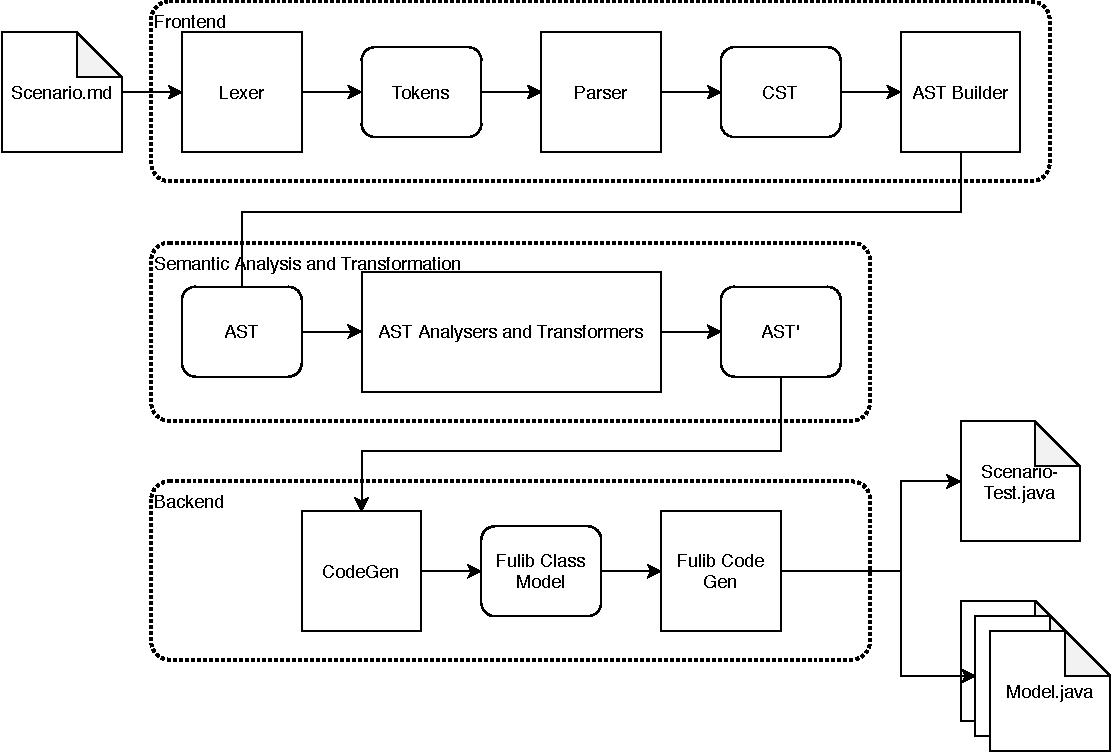
\includegraphics[width=\textwidth]{chapter/fulib-scenarios/img/architecture.pdf}
    \caption{Compiler-Architektur}
    \label{fig:compiler-architecture}
\end{figure}

\subsection{Frontend - ANTLR v4}\label{subsec:frontend-antlr4}

Die Übersetzung der Markdown-Datei beginnt mit deren Einlesen und Umwandeln in verarbeitbare Daten.
Im Compilerbau wird dies klassisch in zwei Phasen unterteilt:
Dem \emph{Lexer}, der die Zeichenfolge in eine Liste von Wörtern mit Typinformationen, genannt \emph{Tokens}, umwandelt;
und dem \emph{Parser}, der die flache Liste von Tokens nach den Regeln der Grammatik in eine Baumstruktur bringt,
die \emph{Concrete Syntax Tree (CST)} genannt wird.

Da die Umwandlung in Tokens und deren Strukturierung Anwendung in den meisten Compilern findet
und deren Implementierung meist nach einem festen Muster stattfindet,
existieren Tools, die diesen Prozess vereinfachen.
Diese werden \emph{Compiler-Compiler} oder \emph{Lexer- und Parsergeneratoren} genannt.

Das Frontend des Scenario-Compilers basiert auf dem Parsergenerator ANTLR4~\cite{antlr4-reference}.
Mit diesem können Grammatiken in einem EBNF-ähnlichen Format spezifiziert werden.
Aus der Grammatik generiert das Tool dann Java-Code, der Dateien einlesen kann und einen CST generiert.

Zunächst soll betrachtet werden, wie die FulibScenarios-Grammatik definiert ist.
Dies beginnt mit der Definition des Lexers.
In Listing~\ref{lst:ScenarioLexer.g4} ist ein Ausschnitt der ANTLR4-Grammatik zu sehen, die diesen definiert.
Der Ausschnitt ist ausreichend um das Scenario aus Listing~\ref{lst:CompilationExample.md} verarbeiten zu können;
die eigentliche Grammatik von FulibScenarios besteht aus vielen weiteren Regeln, um alle Funktionen der Sprache zu implementieren.
Sie ist in Anhang~\ref{sec:scenario-lexer-grammar} zu finden.

\codelisting{antlr}{chapter/fulib-scenarios/grammars}{ScenarioLexer.g4}{Ausschnitt der Scenario-Lexer-Grammatik}

Die Grammatik besteht aus mehreren Regeln, die einem Muster einen Namen zuordnen.
Dieser Name wird später den Tokens zugeordnet.
So haben Tokens mit dem Text \code{and} später den Namen \code{AND};
und jene, die eine Zahl darstellen, den Namen \code{INTEGER}.
Im Folgenden werden Tokens mit der Kurzschreibweise \code{<name>(<text>)} bezeichnet,
z.B.\ \code{AND(and)} und \code{INTEGER(12)}.

Die rechte Seite jeder Regel ähnelt einem regulären Ausdruck.
Bei Schlüsselwörtern wie \code{a}, \code{is} und \code{with} muss der Text exakt entsprechen;
\code{There} darf beispielsweise auch kleingeschrieben werden.
Ein \code{HEADLINE}-Token entsteht, wenn auf ein \code{#}-Zeichen beliebig viele Zeichen und ein Zeilenumbruch folgen.
Ganze Zahlen können mit einem Minus-Zeichen beginnen und bestehen aus mindestens einer Ziffer.
Wörter beginnen mit einem Buchstaben, gefolgt von beliebig vielen Buchstaben, Ziffern, Apostrophen, Unterstrichen und Bindestrichen.
Die Regel \code{WS} sorgt durch die Angabe \code{-> skip} dafür, dass keine Whitespace-Zeichen zu Token werden.
Falls mehrere Regeln infrage kommen würden, wird zunächst die längstmögliche Übereinstimmung angewandt;
falls das nicht eindeutig bestimmbar ist, gewinnt die als erste definierte Regel.
So wird aus dem Text \code{ampersand} nicht die Token-Folge \code{A(a), WORD(mpers), AND(and)}, sondern \code{WORD(ampersand)}.

Wendet man die Regeln aus Listing~\ref{lst:ScenarioLexer.g4} auf das Scenario aus Listing~\ref{lst:CompilationExample.md} an,
so erhält man die in Listing~\ref{lst:CompilationExampleTokens.txt} gezeigte Liste von Tokens.

\codelisting{text}{chapter/fulib-scenarios/trees}{CompilationExampleTokens.txt}{Aus Listing~\ref{lst:CompilationExample.md} abgeleitete Token-Liste}

Als nächstes sollen diese Tokens in einen CST umgewandelt werden.
Dies ist die Aufgabe des Parsers.
Listing~\ref{lst:ScenarioParser.g4} zeigt wieder einen Ausschnitt der Grammatik,
die diesen für das Beispiel-Scenario ausreichend definiert.
Die vollständige Parser-Grammatik ist Inhalt von Anhang~\ref{sec:scenario-parser-grammar}.

\codelisting{antlr}{chapter/fulib-scenarios/grammars}{ScenarioParser.g4}{Ausschnitt der Scenario-Parser-Grammatik}

Die Struktur der Parser-Grammatik ist ähnlich zur Lexer-Grammatik.
Wieder gibt es benannte Regeln, jedoch bestehen deren rechte Seite nicht aus regulären Ausdrücken,
sondern aus \emph{Nicht-Terminal}-Symbolen, die weitere Parser-Regeln referenzieren\footnote{Diese sind in der ANTLR-Grammatik daran zu erkennen, dass sie mit einem Kleinbuchstaben beginnen.},
sowie \emph{Terminal}-Symbolen, die analog Verweise auf Lexer-Regeln sind\footnote{In ANTLR beginnen diese immer mit einem Großbuchstaben.}.
Die \code{thereSentence}-Regel aus Listing~\ref{lst:ScenarioParser.g4} beginnt beispielsweise mit den Terminalen \code{THERE}, \code{IS}, \code{A} und \code{WORD}, gefolgt von dem Nicht-Terminal \code{withClause}.
Beim Ableiten eines konkreten Syntaxbaumes werden alle Terminale zu den Blättern;
die Nicht-Terminale werden zu Elternknoten.

In Listing~\ref{lst:ScenarioParser.g4} dient \code{file} als Startregel.
Nun wird diese Regel \emph{abgeleitet}, d.h.\ die Tokens, die derzeit am Anfang unserer Liste stehen, werden entweder einem Terminal zugeordnet oder ein Nicht-Terminal wird rekursiv abgeleitet.
Da \code{file} mit dem Nicht-Terminal \code{heading} beginnt, wird zunächst dieses abgeleitet.
Dabei wird dem Terminal \code{HEADLINE} das Token \code{HEADLINE(# My First Scenario)} zugeordnet.
Als nächstes werden \code{sentence} und \code{thereSentence} abgeleitet, wobei den Terminalen \code{THERE}, \code{IS} und \code{A} und \code{WORD} das entsprechende Token zugeordnet wird.
Bei der Ableitung von \code{withClause} muss entschieden werden, welche Alternative der Regel zutrifft.
Im Fall von dem Teilsatz \code{with name Alice} wird die erste Alternative ausgewählt, da \code{name} ein \code{WORD}-Token ist und nicht dem \code{INTEGER}-Terminal zugeordnet werden kann.
Der Ausdruck \code{withClause (AND withClause)*} in der \code{thereSentence}-Regel bedeutet, dass auf eine \code{with}-Klausel beliebig viele weitere \code{with}-Klauseln folgen können, solange dazwischen ein \code{AND}-Token steht.
Da dies im Beispiel der Fall ist, wird \code{AND(and)} dem \code{AND}-Terminal zugeordnet und \code{withClause} erneut abgeleitet.
Diesmal wird dabei die zweite Alternative gewählt, da \code{INTEGER(30)} dem \code{INTEGER}-Terminal zugeordnet werden kann.
Zuletzt wird der Punkt am Ende des Satzes dem \code{FULL_STOP}-Terminal zugeordnet.

Nun sind alle Token, die der Lexer aus der Eingabe produziert hat, verbraucht, und der Parse-Vorgang ist abgeschlossen.
Das Ergebnis ist der in Abbildung~\ref{fig:parsetree} sichtbare Syntaxbaum.

\begin{figure}
    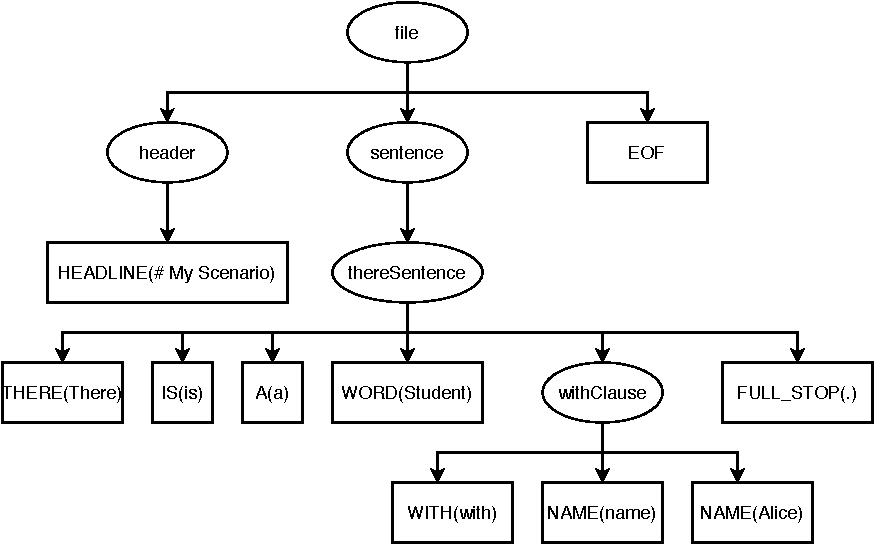
\includegraphics[width=\textwidth]{chapter/fulib-scenarios/img/parsetree.pdf}
    \caption{Syntaxbaum von Listing~\ref{lst:CompilationExample.md}}
    \label{fig:parsetree}
\end{figure}

Der CST ist eng an die Struktur der Grammatik gebunden.
Bei Änderungen an der Grammatik, beispielsweise dem Einfügen von gemeinsamen Hilfsregeln beim Refactoring,
ändert sich auch die Struktur des CST\@.
Würde man also den CST für weitere Schritte des Compile-Vorgangs verwenden,
müsste man die Implementierung dieser Schritte bei Änderung der Grammatik an die neue CST-Struktur anpassen,
was zu einem Wartungsproblem führt.

Deshalb hat das Frontend zusätzlich die Aufgabe, den CST in eine umgänglichere Form umzuwandeln.
Diese nennt man \emph{Abstract Syntax Tree} (AST).
Die Namensgebung folgt daher, dass über die Grammatik abstrahiert wird.

Technisch gesehen besteht der AST aus einem weiteren Datenmodell neben dem Datenmodell des Parsers.
Während letzteres von ANTLR aus der Grammatik hergeleitet und generiert wird,
ist das Datenmodell des AST manuell definiert und am logischen Aufbau eines Szenarios orientiert.
So gibt es AST-Klassen für Pakete, Dateien, Scenarios in Dateien und jegliche Arten von Sätzen und Ausdrücken.
Für bestimmte Konstrukte, die in mehreren Sätzen vorkommen, gibt es Hilfsklassen um Code-Duplizierung zu vermeiden.
Dazu gehören z.B.\ mit Namen versehene Ausdrücke.

Das Datenmodell des AST wird ebenfalls automatisch generiert.
Grund dafür ist, dass jede AST-Klasse lediglich aus Klassenvariablen, Gettern und Settern sowie einer Factory-Methode besteht.
Diese können mit einer Liste von Attributen ausreichend definiert werden.

Die Generierung des AST erfolgt durch das von mir entwickelte GenTreeSrc-Tool~\cite{gentreesrc}.
Dieses erlaubt die Definition von Klassen und Attributen in einer \code{gts}-Datei,
aus der dann Java-Dateien generiert werden.
Listing~\ref{lst:FulibScenarios1.gts} zeigt einen Ausschnitt der \code{gts}-Datei von FulibScenarios,
in dem die für Beispiel~\ref{lst:CompilationExample.md} benötigten Definitionen abgebildet sind.
Die vollständige Definitionsdatei ist in Anhang~\ref{sec:gts-definitions} zu finden.

\codelisting{java}{chapter/fulib-scenarios/definitions}{FulibScenarios1.gts}{Ausschnitt der FulibScenarios.gts-Datei}

Diese Datei verwendet die Syntax von GenTreeSrc, welche wie folgt zu lesen ist:
Auf der obersten Ebene werden Klassen inkl.\ Package-Name definiert, z.B. \code{org.fulib.scenarios. ast.Node}. % space added before ast to allow line break
Das Schlüsselwort \code{abstract} bedeutet hier, dass diese ein Interface ist und nicht instanziiert werden kann.
In den geschweiften Klammern nach einer Klassendefinition werden weitere Klasse definiert, die von dieser erben.
Diese werden entweder im selben Package (\code{org.fulib.scenarios.ast.ScenarioFile}) oder in einem Unterpackage
(\code{org.fulib.scenarios.ast.decl.Name}) abgelegt.
Runde Klammern nach dem Klassennamen enthalten die Attribute, die die Syntax \code{name: Typ} verwenden.
Die Typausdrücke \code{[T]} und \code{[T:U]} stehen für \code{List<T>} und \code{Map<T, U>}.
Einfache Attribute haben einen Getter und Setter;
das Schlüsselwort \code{readonly} sorgt dafür, dass kein Setter erzeugt wird.
Aus jedem Attribut wird ein Parameter im Konstruktor bzw.\ der Factory-Methode der generierten Klasse.

Mit den generierten Klassen kann nun ein AST erzeugt werden.
Dafür implementiert das Frontend einen Übersetzungsschritt für eine Vielzahl von CST-Knoten,
der diese bei den Blättern beginnend in AST-Knoten umwandelt.

Ergebnis der Übersetzung des in Abbildung~\ref{fig:parsetree} gezeigten CST ist der AST,
der in Listing~\ref{lst:CompilationExampleAST.txt} in seinem Ausgabeformat dargestellt ist\footnote{
    Im Scenario-Compiler steht auf der obersten Ebene ein \code{CompilationContext}-Knoten, der u.a.\ Kompilierungsoptionen enthält.
    Darunter befinden sich Knoten für Pakete;
    erst diese enthalten den \code{ScenarioFile}-Knoten.
    Aus Gründen der Einfachheit wurden diese beiden Ebenen hier ausgelassen.
}.

\codelisting{java}{chapter/fulib-scenarios/trees}{CompilationExampleAST.txt}{AST von Listing~\ref{lst:CompilationExample.md}}

\subsection{Analyse und Transformation}\label{subsec:data-model-gentreesrc}

Sobald der AST im Frontend erzeugt wurde, beginnt die Analyse- und Transformationsphase.
Deren Aufgabe ist es, den AST auf semantische Gültigkeit zu überprüfen und ihn so vorzubereiten,
dass in der folgenden Codegenerierungsphase alle Informationen bereitstehen.

Bei der Analyse werden die Fehler- und Warnmeldungen erzeugt, die die Ausgabe des Compilers bilden.
Dafür werden im AST durch das Frontend Positionsinformationen von Tokens hinterlegt, die es ermöglichen,
in den Meldungen Dateinamen, Zeilen- und Spaltennummern einzubringen.
Die entsprechenden Attribute in AST-Klassen wurden hier zur Einfachheit ausgelassen,
sie sind jedoch in Anhang~\ref{sec:gts-definitions} enthalten.

Die Analyse- und Transformationphase besteht im Scenario-Compiler aus zwei logisch getrennten Unterphasen,
der Gruppierung und der Namensauflösung.
Die Gruppierung ist zuständig dafür, aus der linearen Abfolge von Sätzen in einem Scenario eine Baumstruktur zur erzeugen,
wenn Sätze anderen untergeordnet werden können.
Dies ist beispielsweise bei jenen Sätzen der Fall, die unter einem \code{call}-Satz stehen, welche im vorherigen Abschnitt unter~\ref{subsec:methods} näher erläutert wurden.
Jeder Satz, dessen Subjekt dem des \code{call}-Satz entspricht, wird diesem untergeordnet und ist nicht länger direkt Teil der Satzliste des Scenarios.
Grund dafür ist, dass der Code für diese Sätze später nicht im Test, sondern in der entsprechenden Methode auftaucht.
Da für die Bestimmung von Subjekten keine komplexe Namensauflösung notwendig ist,
die Unterordnung von Sätzen jedoch deren Scope beeinflusst, geschieht die Gruppierung vor der Namensauflösung.

Die Namensauflösung bündelt sowohl die direkte Namensauflösung anhand des Scopes,
als auch die Auflösung von Attributen und Assoziationen, das Erzeugen von Klassen, das Erzeugen von Diagnosenachrichten,
und die Umstrukturierung des AST\@.
Grund dafür ist, dass diese Aufgaben eng verzahnt und meist in einem Schritt ausführbar sind.
Beim Auflösen von Assoziation beispielsweise kann diese angelegt werden, falls es sie noch nicht gibt,
andernfalls muss die bestehene Assoziation mit der neuen Definition auf Konsistenz überprüft und ggf.\ eine Fehlermeldung erzeugt werden.
Dies kann z.B.\ auftreten, wenn bei der zweiten Verwendung versehentlich die Rückrichtung falsch benannt wird:

\begin{codeblock}
    Kassel has country and is one of the cities of Germany.
    Berlin has country and is the capital of Germany.
\end{codeblock}

Dies erzeugt die folgende Fehlermeldung in der Konsolenausgabe des Compilers:

\begin{codeblock}
    src/org/example/ErrorExample.md:4:30: error: conflicting redeclaration of reverse association of 'City.country' [association.reverse.conflict]
    was: Country.cities, association to many 'City'
    now: Country.capital, association to one 'City'
\end{codeblock}

Die Fehlermeldungen sind so strukturiert, dass sie alle nötigen Informationen zur Lösung des Problems enthalten:
Zu Beginn stehen Dateiname, Zeile und Spalte, die mit einer IDE direkt an der richtigen Stelle geöffnet werden können.
Nach der Angabe, um was für eine Art Meldung es sich handelt (hier \code{error}, auch möglich \code{syntax}, \code{warning} und \code{note}),
folgt eine kurze Beschreibung.
In den eckigen Klammern steht eine feste ID der Fehlerart, nach der leicht bei Google oder StackOverflow gesucht werden kann.
Dadurch kann auch die Formulierung der Beschriebung geändert oder in eine andere Sprache übersetzt werden,
wonach Online-Suchergebnisse weiterhin auffindbar sind.
Viele (Fehler-)Meldungen enthalten außerdem einige Zeilen mit Extra-Informationen,
wie hier die Informationen zur vorherigen und jetzigen Deklaration der Assoziation.
Diese sollen den Entwickler ebenfalls bei der Problembehebung unterstützen.

Eine weitere zur Transformationsphase gehörende Aufgabe ist es, den AST vor der Auflösung zu vereinfachen.
Bildet man beispielsweise eine Art von AST-Knoten immer auf eine andere ab,
müssen folgende Schritte nicht mehr für die erste Knotenart implementiert werden,
da man sichergehen kann, dass sie nicht mehr vorkommt.
Dadurch kann Code-Duplizierung vermieden und die Code-Generierung vereinfacht werden.

Es soll nun der im vorherigen Abschnitt angelegte AST, der in Listing~\ref{lst:CompilationExampleAST.txt} gezeigt wurde, weiter verarbeitet werden.
Da die Gruppierung in diesem Beispiel keine Veränderungen durchführt, können wir als nächstes die Namensauflösung betrachten.
Dabei führt der Scenario-Compiler zunächst einen Umformungsschritt durch, der den \code{ThereSentence} durch einen \code{IsSentence} und einen \code{HasSentence} ersetzt.
Diese Umformung erhält die Semantik, dass ein Objekt angelegt und einer Variable zugewiesen wird und daraufhin ein Attribut gesetzt wird,
wie im vorherigen Abschnitt unter~\ref{subsec:simple-sentences-and-expressions} gezeigt wurde.
In Listing~\ref{lst:PreprocessedAST.txt} ist der AST nach dieser Umformung abgebildet.
Zur Vereinfachung ist nur der \code{Scenario}-Knoten gezeigt;
der \code{ScenarioFile}- sowie darüberliegende Knoten bleiben unverändert.
Listing~\ref{lst:FulibScenarios2.gts} zeigt die neuen AST-Klassendefinitionen, die dafür notwendig sind.

\codelisting{java}{chapter/fulib-scenarios/trees}{PreprocessedAST.txt}{AST nach Umformung von \code{ThereSentence} zu \code{IsSentence} + \code{HasSentence}}

\codelisting{java}{chapter/fulib-scenarios/definitions}{FulibScenarios2.gts}{Neue AST-Klassendefinitionen für Listing~\ref{lst:PreprocessedAST.txt}}

Im nächsten Schritt werden die neu erzeugten \code{Sentence}-Knoten aufgelöst.
Meist ist an dem Wort \code{Unresolved} zu erkennen, dass ein AST-Knoten aufgelöst werden muss.
Im \code{IsSentence}-Knoten fällt dabei der \code{type} der \code{CreationExpr} auf.

Der Compiler verwendet für die Auflösung einen Scope, der aus mehreren Ebenen besteht die jeweils Deklarationen bereitstellen können.
Beim Auflösen eines Namens wird beginnend beim inneren Scope eine Deklaration mit diesem Namen gesucht;
falls dies kein Ergebnis liefert wird im jeweils nächstäußeren Scope gesucht.
Gelangt man im äußersten Scope an ohne eine Deklaration gefunden zu haben,
kann diese automatisch erzeugt werden oder eine Fehlermeldung generiert werden.
Dies findet wieder auf der zuständigen Scope-Ebene statt.

Die Scope-Hierarchie ist im Fall der \code{CreationExpr} von außen nach innen wie folgt:
Global, Paket, Scenario-Datei, Scenario, Satz-Liste.
Dabei ist die Satz-Liste für das Auflösen und Anlegen von lokalen Variablen zuständig,
die Scenario-Datei und Paket enthalten Hilfsmethoden bzw.\ Klassen,
und der globale Scope stellt extern importierte Klassen bereit.
Wird nun versucht, den Typnamen \code{Student} in diesem Scope aufzulösen,
findet man zunächst keine entsprechende Deklaration.
Deshalb wird ein neues Objekt im Datenmodell des Compilers angelegt,
das die Klasse \code{Student} repräsentiert und deren Zugehörigkeit zum gleichen Paket wie die Scenario-Datei darstellt.
Der \code{UnresolvedType}-Knoten wird zu einem \code{ClassType}, der auf diese neue Klasse verweist.
Nun ist der Typ der \code{CreationExpr} aufgelöst und kann als Typ der Variable \code{alice} inferiert werden.

Als nächstes muss der \code{UnresolvedName(value: "Alice")} im \code{HasSentence} ersetzt werden.
Der \code{HasSentence} fügt der Scope-Hierarchie eine weitere Ebene hinzu, die den Namen \code{alice} \emph{versteckt}.
Deshalb wird die gleichnamige Variable \emph{nicht} dem \code{UnresolvedName} zugeordnet.
Wäre dies der Fall, würde der \code{has}-Satz eine Assoziation von \code{Student} zu sich selbst erzeugen,
was offensichtlich nicht gewollt ist.
Da \code{alice} nicht aufgelöst werden kann, werden sowohl der \code{UnresolvedName} als auch der umgebende \code{NameAccess} durch ein \code{StringLiteral} ersetzt.

Die Auflösung von \code{UnresolvedName(value: "name")} als Teil der \code{NamedExpr} wird besonders gehandhabt.
Hier erfolgt nicht wie üblich eine Suche im aktuellen Scope,
sondern im Typ des Empfängers, also des \code{object}s des \code{HasSentence}.
Dies ist der Typ der Variable \code{var1}, der beim Auflösen des \code{IsSentence} als der Klassentyp \code{Student} inferiert wurde.
Nun wird in diesem nach einem Attribute oder einer Assoziation namens \code{name} gesucht.
Wäre eines davon bereits vorhanden, würde der Compiler diverse Überprüfungen durchführen,
ob diese mit dem Typ des Attributwerts kompatibel sind.
Da die Klasse \code{Student} jedoch bisher noch keine Attribute oder Assoziationen hat,
wird ein neues Attribute mit dem Namen \code{name} und dem Typ \code{String} angelegt
und im Datenmodell der Klasse \code{Student} gespeichert.
Daraufhin wird der \code{UnresolvedName} durch einen \code{ResolvedName} ausgetauscht,
der auf das neue Attribute verweist.

Die Analyse und Transformation des AST ist nun abgeschlossen.
Listing~\ref{lst:FinalAST.txt} zeigt den vollständigen AST, der nun für die Codegenerierung vorbereitet ist.
Die darin verwendeten neuen AST-Definitionen sind in Listing~\ref{lst:FulibScenarios3.gts} zu finden.

\codelisting{java}{chapter/fulib-scenarios/trees}{FinalAST.txt}{AST nach Analyse und Transformation}

\codelisting{java}{chapter/fulib-scenarios/definitions}{FulibScenarios3.gts}{Für Auflösung und vollständingen AST benötigte AST-Definitionen}

\subsection{Codegenerierung - Fulib}\label{subsec:codegen-fulib}

% Intro
Die letzte Aufgabe des Scenario-Compilers ist die Codegenerierung.
Dabei werden mit den in vorherigen Phasen gesammelten Informationen neue Java-Dateien erzeugt bzw.\ bestehende verändert.
Der Scenario-Compiler verwendet für diesen Zweck die Fulib\cite{fulib}-Bibliothek.
Diese stellt wie der Scenario-Compiler ein Datenmodell für Klassen, Attributen, Assoziationen und Methoden bereit,
bietet aber auch deren Umwandlung in Java-Code an.
Der Codegenerator von Fulib unterstützt dabei das Zusammenführen von bestehenden Java-Dateien mit neu generiertem Code,
wodurch er mit handgeschriebenem Code kompatibel ist.

% Model vs Test Classes
Der Scenario-Codegenerator sieht eine logische Trennung von Modell und Tests vor.
Fulib selbst kennt diese Trennung nicht, daher erzeugt der Scenario-Compiler zwei getrennte Fulib-Datenmodelle, welche später auch in getrennte Verzeichnisse Java-Dateien ablegen.
Test-Klassen und -Methoden werden ansonsten vom Scenario-Compiler bei der Codegenerierung wie Modelklassen behandelt,
sind daher hier nicht näher erläutert.

% Model Conversion
Zu Beginn der Codegenerierung konvertiert der Scenario-Compiler sein internes, an die Scenario-Sprache angepasstes Datenmodell in das Datenmodell von Fulib.
Für Klassen, Attribute und Assoziationen ist diese Umwandlung annähernd 1-zu-1;
lediglich Methoden werden gesondert gehandhabt.
Grund dafür ist, dass das Datenmodell von Fulib zwar Methodendeklarationen versteht,
deren Rumpf jedoch als Zeichenkette modelliert,
da es kein Modell für Anweisungen und Ausdrücke bereitstellt.
Der Scenario-Compiler ist also dafür zuständig, Methodenrümpfe zeilenweise zusammenzusetzen.
Dafür ist für jede Satzart eine Regel definiert, die anhand der in der Analyse- und Transformationsphase gesammelten Informationen eine oder mehrere Java-Anweisungen erzeugt.
Ähnlich werden Ausdrücke der Scenario-Sprache in Java-Ausdrücke übersetzt.
Dabei wird in einer Zeichenkette der Methodenrumpf zusammengebaut.
Zuletzt wird im Datenmodell von Fulib ein Objekt angelegt, das diese Zeichenkette sowie Name, Rückgabetyp und Parameter der Methode speichert.

% New Files
Mit dem fertig bestückten Datenmodell kann Fulib dann die Java-Dateien erzeugen bzw.\ verändern.
Beim Anlegen neuer Dateien ist dieser Prozess relativ einfach.
Es genügt, für Attribute, Assoziationen und Methoden einige Vorlagen zu definieren,
die diese in Zeichenketten umwandeln.
Diese werden dann aneinandergehängt und in die entsprechende Datei geschrieben.

% Existing Files - Parsing and Fragments
Existiert die Zieldatei jedoch schon, ist der Prozess deutlich aufwändiger.
Zunächst wird der Java-Code mit einem Parser eingelesen, um die Position und Signatur der Deklarationen in der Datei zu ermitteln.
Daraus werden die sogenannten \emph{Fragmente} gebildet, welche die Datei in Abschnitte aufteilen.
Listing~\ref{lst:StudentFragments.java} zeigt, wie eine bestehende Java-Datei in Fragmente aufgeteilt wird.
Darin deutet ein Kommentar der Form \jcode{// <kind>:<signature>} den Beginn eines Fragments an.

\codelisting{java}{chapter/fulib-scenarios/java}{StudentFragments.java}{Fragmente einer Java-Datei}

% Listing Explanation
Hier ist zu erkennen, dass aus jeder Art von Deklaration (Klasse, Variable, Methode) ein Fragment wurde.
Auch aus anderen Deklarationen wie Imports oder Package-Angaben, die hier nicht gezeigt sind,
werden Fragmente.
I.d.R.\ bildet der Name der Deklaration die Signatur,
bei Methoden nehmen jedoch auch die Parametertypen Einfluss darauf.
Diese müssen bei der korrekten Handhabung von überladenen Methoden beachtet werden.
Auffällig ist auch, dass die Leerzeilen zwischen den Deklarationen zu Fragmenten wurden, die mit \code{gap:} bezeichnet wurden.
Dies ermöglicht die spätere Reproduktion dieser Formattierung.

% Templates
Die Vorlagen für Attribute, Assoziationen und Methoden lassen sich ebenfalls als Fragmente verwenden.
Ein Attribut hat beispielsweise vier Vorlagen, je eine für die Konstante, die Variable, und die Getter- und Setter- Methoden.
In diesem Beispiel wurde die Variable \code{name} sowie deren Getter bereits von Hand geschrieben.
Es fehlen also in der bestehenden Datei der Setter von \code{name} sowie die zugehörige Konstante.

% Merging Fragments
Nun gilt es, die Fragmente für die neuen Deklarationen in die bestehenden zu integrieren.
Falls ein neues Fragment die gleiche Signature wie ein altes hat, wird das alte ausgetauscht.
Andernfalls wird das neue Fragment an der richtigen Stelle eingefügt.
Bei Deklarationen auf Klassenebene ist dies vor dem Klassenende;
Fragmente für Imports werden beispielsweise vor dem Klassenbeginn eingeordnet.
In Listing~\ref{lst:StudentFinal.java} ist das Ergebnis der Zusammenführung zu sehen.

\codelisting{java}{chapter/fulib-scenarios/java}{StudentFinal.java}{Fragmente der Java-Datei nach Einfügen von generiertem Code}

% Listing Explanation
Das Beispiel zeigt, dass die Variable sowie die manuell definierte Methode unverändert blieben.
Der Getter jedoch wurde überschrieben, wodurch die enthaltene Kommentarzeile gelöscht wurde.
Am Ende der Klasse wurden die Konstante sowie der Setter eingefügt.
Fügt man die Fragmente nun zusammen, erhält man die fertige Java-Datei.
Damit ist die Codegenerierung beendet.


	\chapter{fulib.org}\label{ch:fulib.org}

Fulib.org ist eine interaktive Webseite, welche parallel zu FulibScenarios entwickelt wurde.
Sie bietet einen Editor für Scenarios, die sich direkt kompilieren und ausführen lassen.
Dabei können Ergebnisse wie der erzeugte Java-Code, Klassen- und Objektdiagramme direkt angezeigt werden.
Vorteil dieser Web-basierten Umgebung ist, dass man keinerlei Installationsaufwand betreiben muss, um die Scenario-Sprache auszuprobieren.
Zudem erlaubt die Webseite die Verwendung von Mobilgeräten wie Smartphones oder Tablet-PCs\@.
Die Hauptseite von fulib.org mit dem interaktiven Editor wird in Abschnitt~\ref{sec:main-page} betrachtet.
Zudem bietet fulib.org Möglichkeiten zum Anfertigen, Veröffentlichen und Lösen von Aufgabenblättern und Online-Kursen.
Diese wird in Abschnitt~\ref{sec:assignments} beschrieben.
Zuletzt enthält Abschnitt~\ref{sec:architecture} eine Beschreibung der Architektur der Webseite aus technischer Sicht.

Die Version von fulib.org, auf die sich diese Arbeit bezieht, ist abrufbar unter dem folgenden Link:

\begin{center}
    \url{https://assignments.fulib.org}
\end{center}

Die öffentliche Live-Version ist unter \url{https://www.fulib.org} erreichbar, kann aber von der folgenden Beschreibung in Form und Funktionalität abweichen.

\section{Hauptseite}\label{sec:main-page}

Die Hauptseite erreicht man, wenn man fulib.org das erste mal öffnet.
Dabei präsentiert sich der sogenannte Vier-Panel-Editor, welcher in Abbildung~\ref{fig:four-pane-editor}.

\begin{figure}
    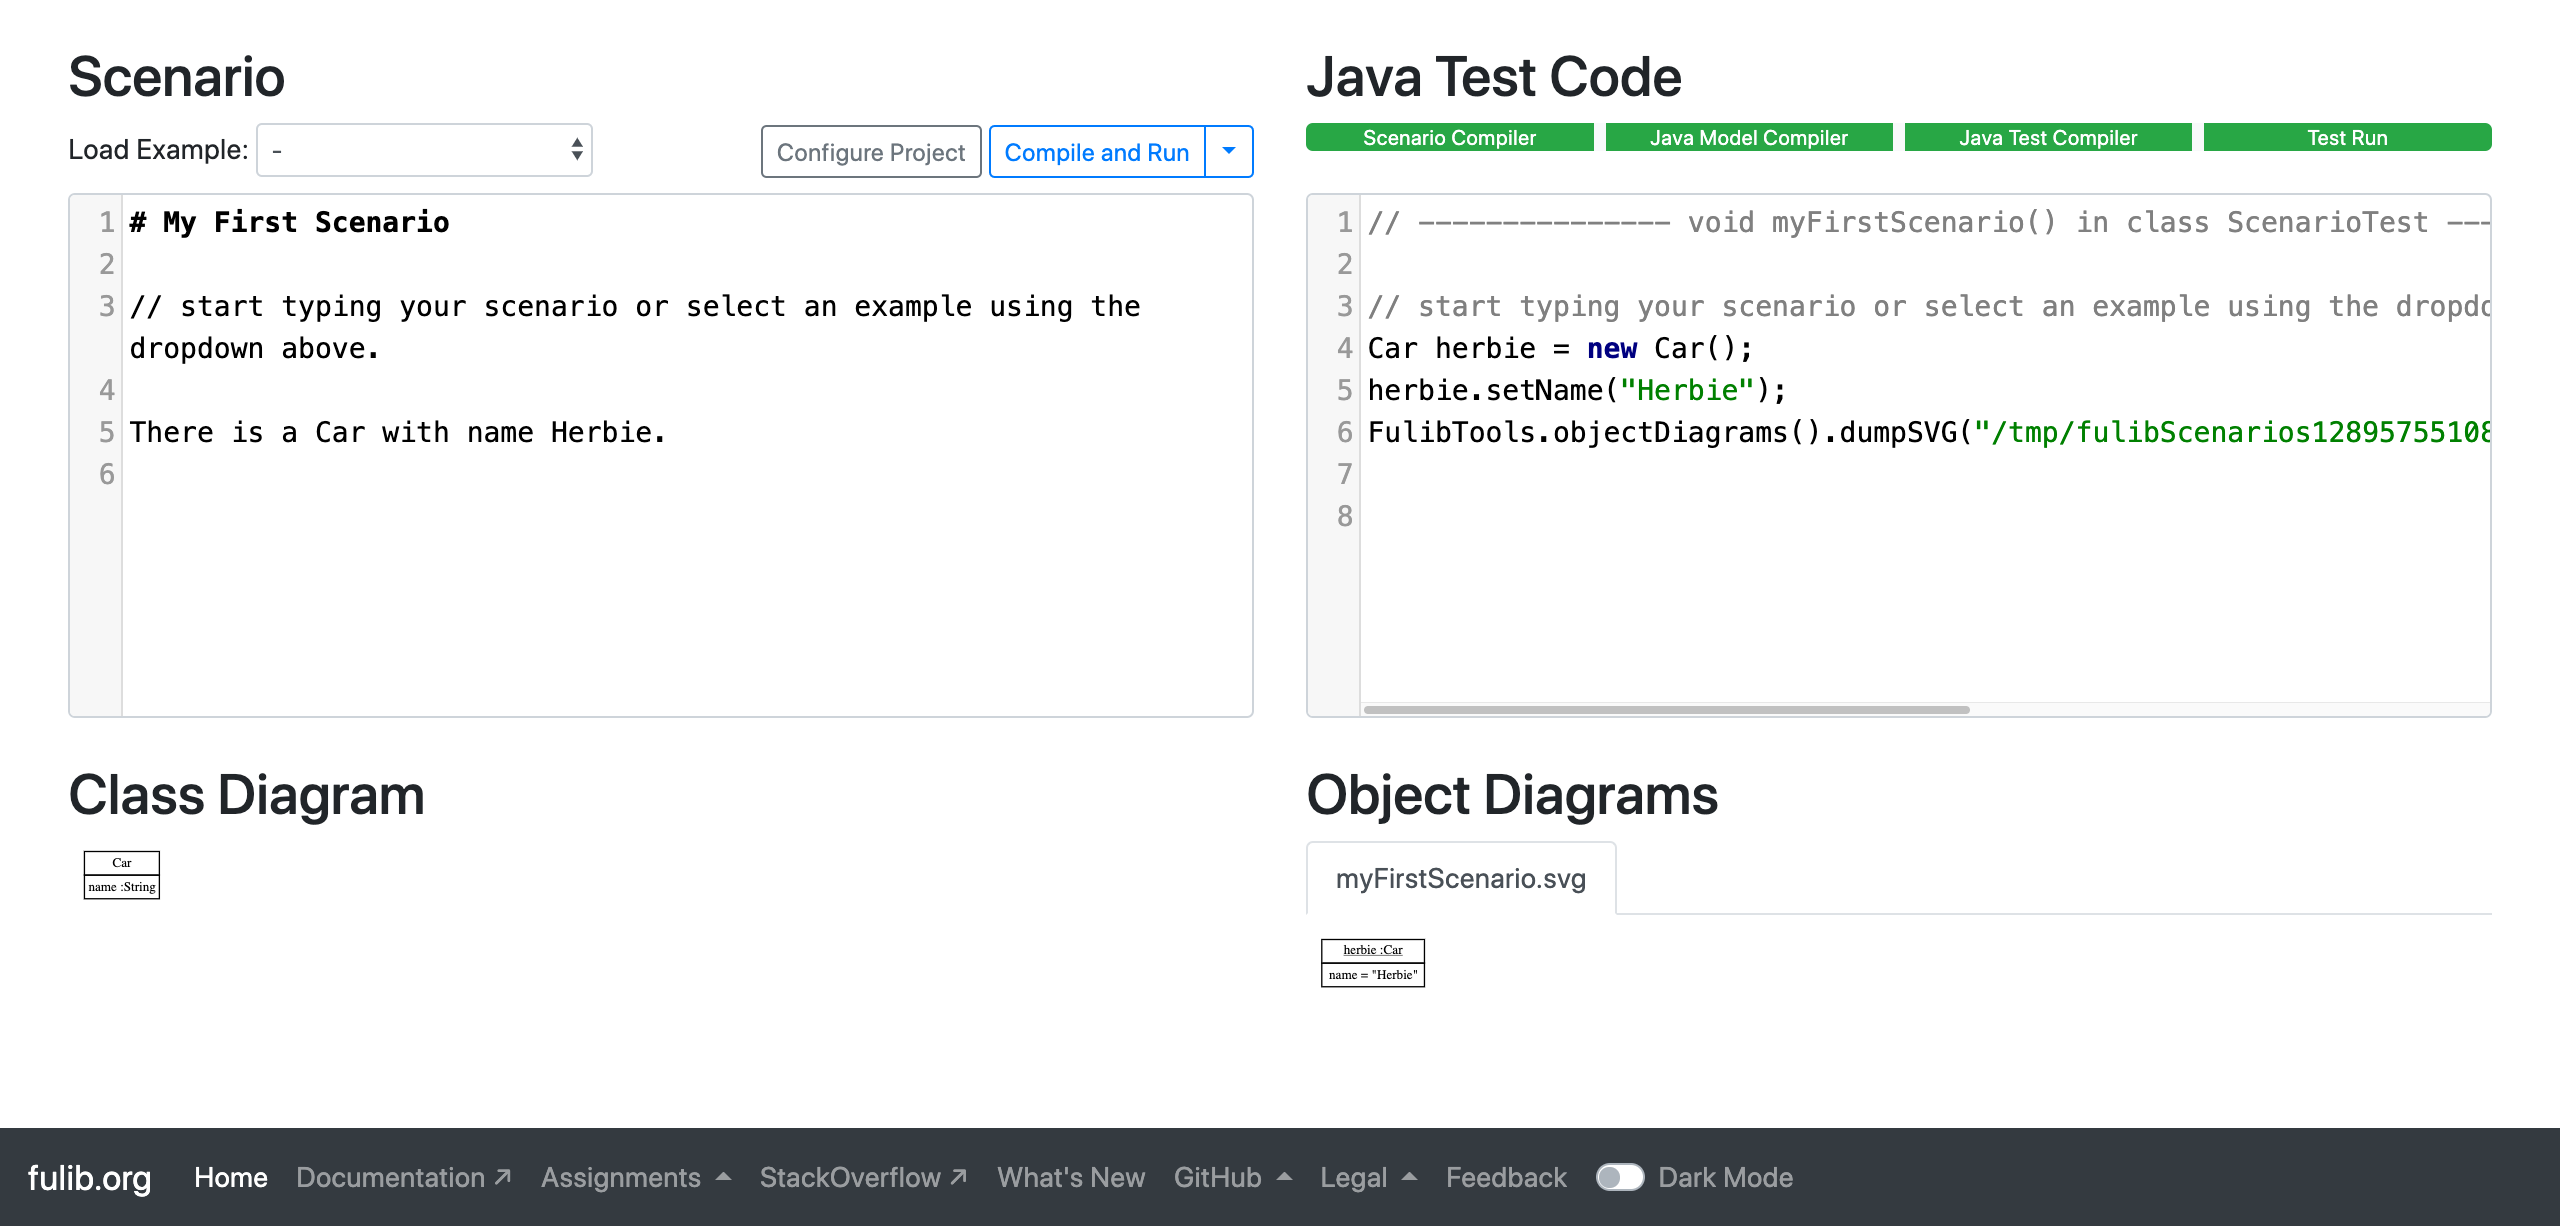
\includegraphics[width=\textwidth]{chapter/fulib.org/img/four-pane-editor.png}
    \caption{Der Vier-Panel-Editor auf der Hauptseite von fulib.org}
    \label{fig:four-pane-editor}
\end{figure}

Dieser zeigt oben links den Scenario-Editor sowie darüber dessen Toolbar.
Oben rechts gibt es ein Fenster für den generierten Java-Code, das auch die Konsolenausgabe des Compilers enthält.
Darüber zeigt eine Statusleiste, ob das Kompilieren und Ausführen erfolgreich war und wenn nicht, welches Tool fehlgeschlagen ist.
Im unteren Teil werden links das Klassendiagramm und rechts Objektdiagramme dargestellt.

Am unteren Rand der Seite befindet sich stets der Footer.
Dieser enthält Links zur Navigation innerhalb der Seite und zu externen Referenzen.
Außerdem finden sich darunter die Einstellungen für Datenschutz,
Möglichkeiten zum Hinterlassen von Feedback und zum Einsehen von Änderungen,
und die Schaltfläche zum Wechseln in den Nachtmodus.

\subsection{Interaktiver Spielplatz}\label{subsec:interactive-playground}

Die wichtigste Funktion der Hauptseite ist der Scenario-Editor.
Gibt man darin ein Scenario ein und klickt auf ``Compile and Run'' oder wartet einen Moment,
wird daraus Java-Code generiert und dessen Tests mit JUnit ausgeführt.
Das dabei entstehende Klassendiagramm sowie Objektdiagramme werden dann in den entsprechenden Bereichen angezeigt.
Um das sofortige Feedback zu erleichtern, wird das Scenario immer automatisch ausgeführt, wenn es länger als eine Sekunde unverändert blieb.
Somit muss man nicht manuell auf ``Compile and Run'' klicken.
Alternativ kann die automatische Ausführung im Dropdown neben dem ``Compile and Run''-Button deaktiviert werden.
Händisch lässt es sich dann immernoch durch Klick oder Verwenden der Testenkürzel auslösen.

Im Fenster für den Java-Code werden die Rümpfe sämtlicher Methoden angezeigt, die im Scenario verwendet wurden.
Davon ausgenommen sind aufgrund ihrer Trivialität Getter und Setter sowie diverse standardmäßig generierte Methoden.
Die Ausgabe des Scenario- und Java-Compilers sowie der JUnit-Testausführung werden ebenfalls in diesem Fenster angezeigt.
Dabei sind die Meldungen des Scenario-Compilers besonders relevant, da diese auf Fehler im Scenario hinweisen.

Objektdiagramme werden unter Tabs angeordnet.
Dies vermeidet Unübersichtlichkeit bei der Verwendung von vielen Diagram-Sätzen im Scenario.
Die einzelnen Darstellungen lassen sich dann getrennt voneinander betrachten.

\subsection{Tutorials}\label{subsec:tutorials}

Über dem Scenario-Editor befindet sich ein Auswahlfeld für vordefinierte Tutorials.
Wählt man eines davon aus, wird dessen Scenario-Text in den Editor übernommen und sofort ausgeführt.
Die Tutorials sind in Kategorien angeordnet und haben bauen in ihrer Reihenfolge aufeinander auf.
Somit werden die behandelten Sprachkonzepte zunehmend komplexer.

In den Tutorial-Scenarios ist beschreibender Text mit \code{//}-Kommentaren realisiert.
Diese bewirt, dass der Text auch im Java-Code auftaucht, was die Zuordnung vereinfacht.
Durch Abschnitte erfolgt eine visuelle Trennung von unabhängigen Teil-Scenarios.

Am Ende jedes Tutorials gibt es Links zu entsprechenden Abschnitten in der Dokumentation,
die detaillierte Informationen zu den verwendeten Sprachkonzepten enthalten.
Dazu gehören auch Grammatiken und häufige Problemfälle.

Die von Tutorials stammenden Scenarios können frei verändert werden.
Dadurch können die Sprachkonzepte direkt ausprobiert werden.
Lädt man das entsprechende Tutorial erneut, wird das vordefinierte Scenario verwendet und die Änderungen verworfen.

\subsection{Projektstarter}\label{subsec:project-starter}

\todo{
Gradle.
}

\subsection{Sicht der Studenten}\label{subsec:students-view}

\todo{
Feedback-Funktion.
Allgemeine Bewertung (PM).
Wünsche.
}

\subsection{Datensammlung}\label{subsec:data-collection}

\todo{
Request-Logging.
Fehleranalyse.
Lernverlauf.
Privacy-Einstellungen.
}

\section{Assignments}\label{sec:assignments}

Assignments bezeichnen ein Feature von fulib.org, das sich mit dem Anlegen, Lösen und Bewerten von Aufgabenblättern sowie Online-Kursen beschäftigt.
Es handelt sich dabei um Modellierungsaufgaben in der Scenario-Sprache.
Diese können sowohl automatisch geprüft als auch manuell bewertet werden.
In diesem Kapitel wird der chronologische Ablauf beschrieben, der bei Aufgabenblättern durchlaufen wird.
Der Unterabschnitt~\ref{subsec:creation} befasst sich zunächst mit deren Anlegen aus Sicht des Kursleiters.
Daraufhin wird unter~\ref{subsec:solution} der Lösungsvorgang aus Perspektive der Studierenden erläutert.
In Unterabschnitt~\ref{subsec:correcting} wird als letzten Schritt das Vorgehen der Korrekteure zum Bewerten der Lösungen beschrieben.
Weiterführend wird die Kurs-Funktion unter~\ref{subsec:courses} vorgestellt, welche die Gruppierung von Aufgabenblättern sowie das selbstständige und unbeaufsichtigte Lernen in größeren Themengebieten ermöglichen.
Zuletzt widmet sich Unterabschnitt~\ref{subsec:assignment-pattern-matching} einem vollständigem Beispielassignment, das die im vorherigen Kapitel eingeführte Mustererkennung einsetzt.

\subsection{Anlegen}\label{subsec:creation}

Das Anlegen von Assignments ist mit dem in Abbildung~\ref{fig:create-assignment} gezeigten Formular möglich.
Dafür muss lediglich im stets sichtbaren Seitenfooter unter ``Assignments'' der Menüeintrag ``Create Assignment'' ausgewählt werden.

\begin{figure}
    \centering
    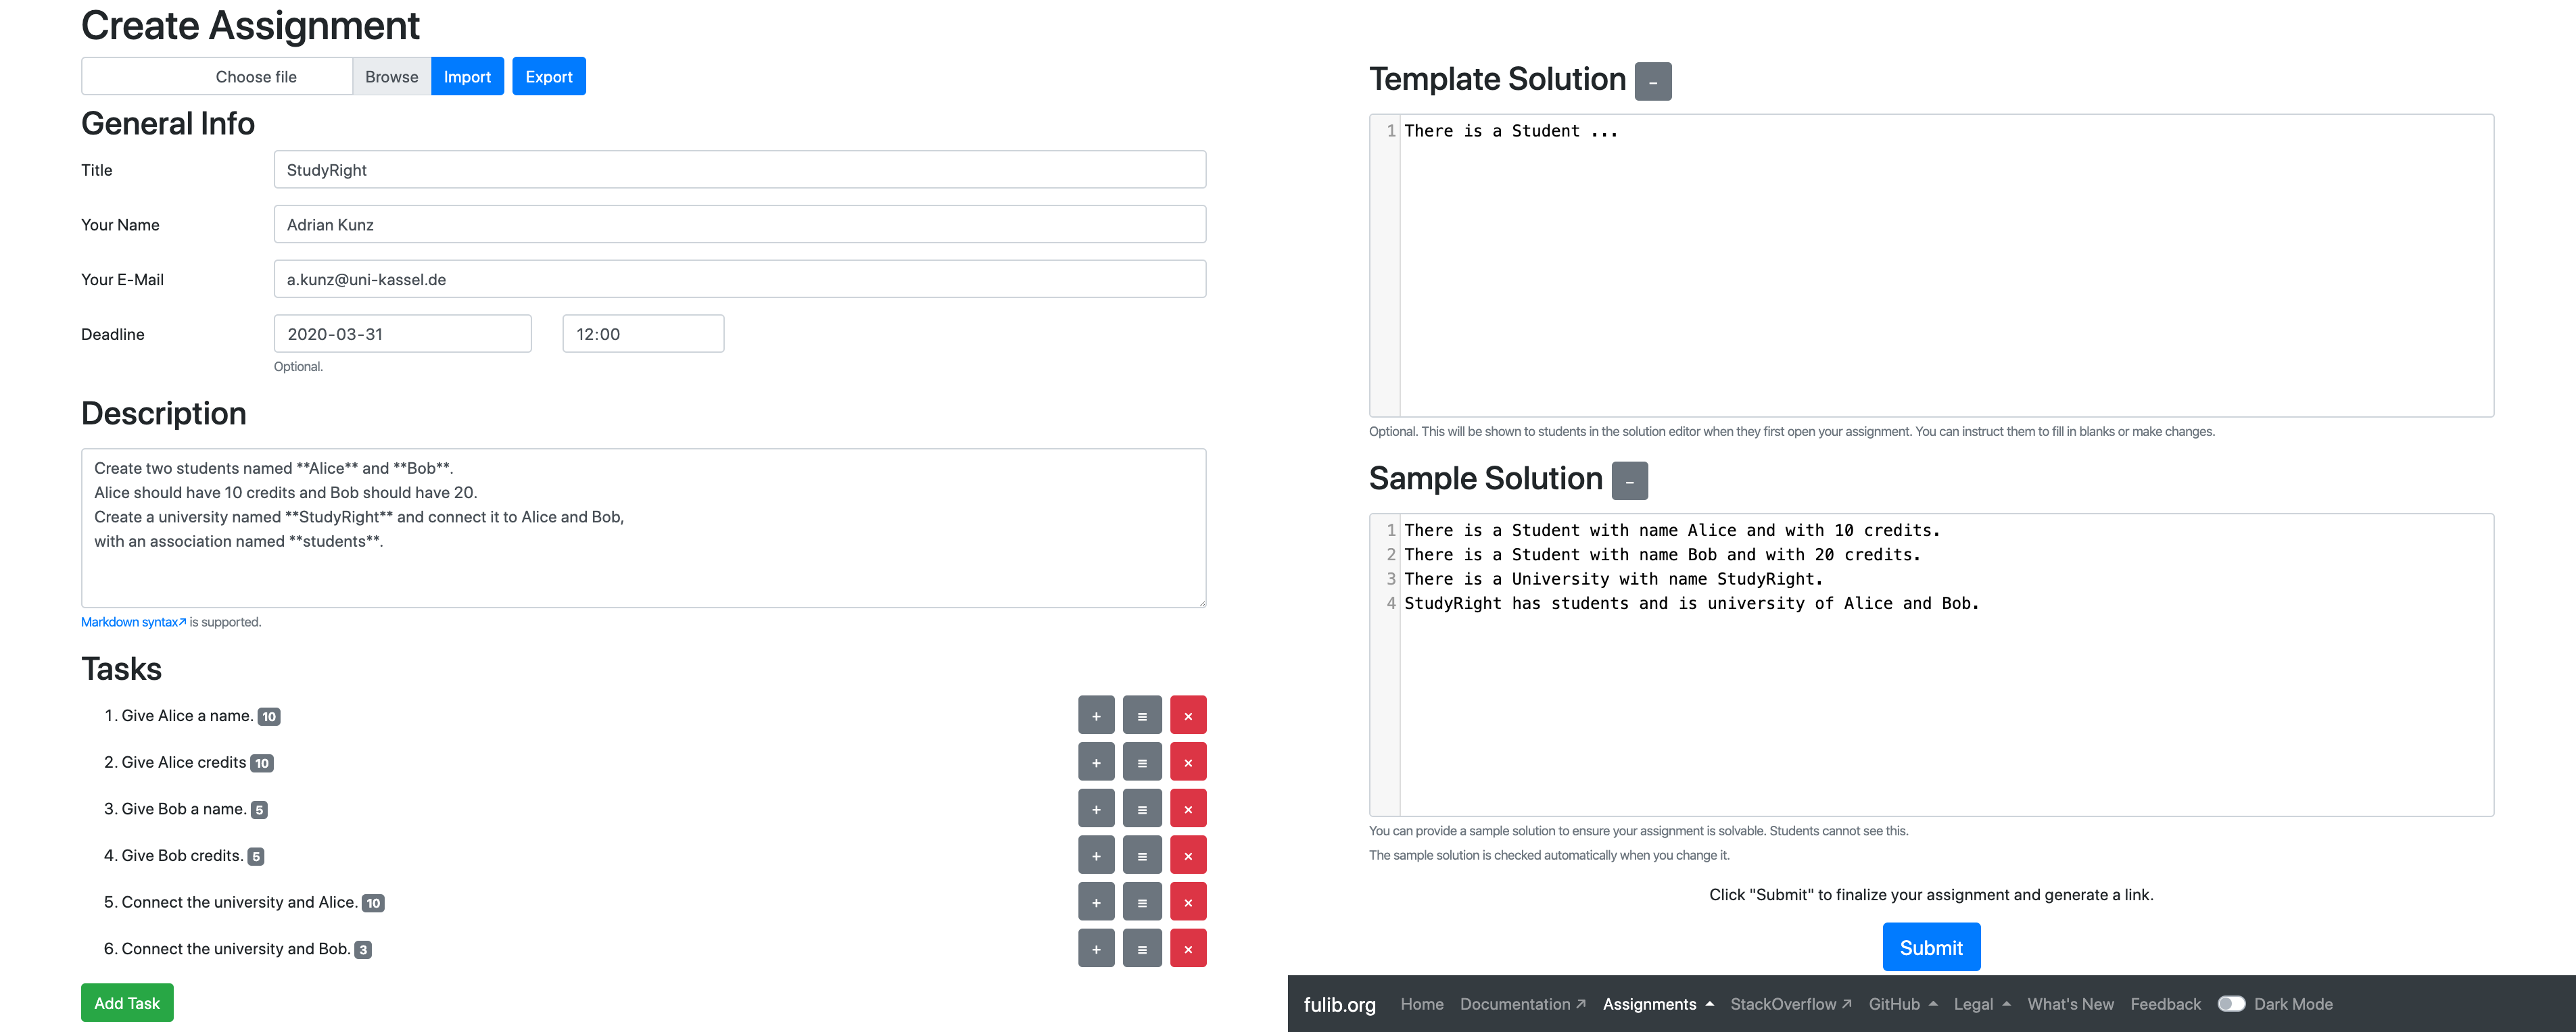
\includegraphics[width=\textwidth]{chapter/fulib.org/img/create-assignment.png}
    \caption{Formular zum Anlegen von Assignments}
    \label{fig:create-assignment}
\end{figure}

Hier werden zunächst der Titel des Assignments sowie Name und E-Mail-Adresse des Kursleiters eingetragen.
Ebenso kann eine Deadline festgelegt werden.
Das mit ``Description'' bezeichnete Feld ist für die Aufgabenstellung vorgesehen.
Dabei wird Markdown-Syntax unterstützt;
es können folglich Überschriften, Tabellen, Listen, Bilder etc.\ eingebracht werden.

Als Nächstes werden die Teilaufgaben (Tasks) eingetragen.
Mit dem Button ``Add Task'' kann der Liste ein neuer Task hinzugefügt werden.
Jeder Task hat eine kurze Beschreibung und eine maximal erreichbare Punktzahl.
Der mit ``Verification'' bezeichnete Editor ist dafür vorgesehen, einen Teil eines Scenarios mit Expect-Sätzen einzutragen.
Ein Task wird später wie folgt automatisch bewertet:
Zunächst wird das unter ``Verification'' eingetragene Teilscenario an die Lösung des Studierenden angehängt.
Das entstehende Scenario wird dann kompiliert und die entstandenen Tests werden ausgeführt.
Erzeugt dies einen Compilerfehler und schlägt der Test fehl, gilt die Teilaufgabe als nicht bestanden und wird mit null Punkten bewertet.
Andernfalls wird die maximal erreichbare Punktzahl vergeben.

Dies lässt sich an einem einfachen Beispiel demonstrieren.
Angenommen, die Beschreibung eines Tasks lautet, dass ein Objekt \code{alice} mit dem Wert \code{Alice} in einem Attribut \code{name} erstellt werden soll.
Der folgende Verifikationscode könnte dies prüfen:

\begin{mdcodeblock}
    We expect that alice has name 'Alice'.
\end{mdcodeblock}

Eine mögliche Lösung wäre dann folgender Satz:

\begin{mdcodeblock}
    There is a Student with name Alice.
\end{mdcodeblock}

Bei deren Prüfung wird diese automatisch mit dem Verifizierungscode in ein vollständiges Scenario verpackt:

\begin{mdcodeblock}
    # Scenario
    There is a Student with name Alice.
    ## Verification
    We expect that alice has name 'Alice'.
\end{mdcodeblock}

Wird dieses kompiliert und der entstehende JUnit-Test ausgeführt, ist dieser erfolgreich.
Folglich wird auf den Task die volle Punktzahl vergeben.
Andererseits entspricht die folgende Lösung nicht der Aufgabenstellung:

\begin{mdcodeblock}
    There is a Student with name Bob.
\end{mdcodeblock}

Fügt man die Lösung wie oben mit dem Verifizierungscode zusammen und kompiliert das Resultat, wird der Scenario-Compiler aufgrund der fehlenden Variable \code{alice} eine Fehlermeldung bei \code{alice has name ...} erzeugen.
Die Fehlermeldung wird als Nichterfüllung des Tasks aufgefasst, wodurch er mit null Punkten bewertet wird.

Zur Übersichtlichkeit lassen sich die einzelnen Tasks mit dem ``+''- bzw.\ ``-''-Button ein- und ausklappen.
Mit der Schaltfläche rechts davon lassen sich Tasks durch Ziehen mit Maus bzw.\ Finger anordnen.
Der rote ``$\times$''-Button löscht den Task aus der Liste.

Unter der Task-Liste befinden sich die Eingabefenster für die Lösungsvorlage (Template Solution) und die Musterlösung (Sample Solution).
Beide lassen sich mit den entsprechenden Buttons ein- und ausklappen, um das Formular übersichtlicher zu machen.
Gibt man eine Vorlage an, so wird diese den Studierenden als Lösung vorgegeben, wenn sie das Assignment öffnen.
Die Aufgabenstellung könnte dann beispielsweise sein, dass das vorgegebene Scenario angepasst oder vervollständigt wird.
Dafür könnten mit ``\code{...}'' Lücken in der Vorlage gelassen werden, welche die Studierenden ausfüllen sollen.
Für das zuvor genannte Beispiel wäre beispielsweise \code{There is a ...} als Vorgabe möglich.

Die Musterlösung ist zwar optional, sie erlaubt jedoch dem Ersteller, seine Aufgabenstellung auf Lösbarkeit zu prüfen.
Dadurch können Fehler in der Aufgabenstellung oder der Verifizierung frühzeitig erkannt werden.
Bei Änderung der Musterlösung wird sie automatisch geprüft.
In der Task-Liste werden dann diejenigen Tasks rot markiert, deren Verifizierung fehlgeschlagen ist.
Dies deutet an, dass es entweder ein Problem in der Musterlösung oder im Verifizierungscode eines Tasks gibt.

Sämtliche Änderungen am Formular werden sofort im Browser gespeichert.
Dadurch wird Datenverlust beim Verlassen der Seite oder bei Ausfall der Internetverbindung vermieden.
Dennoch gibt es die Möglichkeit, den Entwurf des Assignments als Datei auf der Festplatte zu speichern.
Dies ist mit dem ``Export''-Button möglich.
Später kann die Datei dann wieder in das Formular übernommen werden, indem sie im Feld neben dem ``Import''-Button ausgewählt und anschließend auf diesen geklickt wird.
Die Import/Export-Funktion erlaubt ferner, ein Assignment für die spätere Bearbeitung zu speichern und ein neues zu erstellen.
Heruntergeladene Dateien können weiterhin über E-Mail oder Dateifreigabe an andere weitergegeben werden, die das Assignment dann importieren und prüfen oder verändern können.

Um ein fertiges Assignment zu veröffentlichen, genügt ein Klick auf den ``Submit''-Button.
Dieser bewirkt, dass das ausgefüllte Formular an den Server gesendet wird, der das erstellte Assignment speichert und zwei Links generiert.
Abbildung~\ref{fig:create-assignment-success} zeigt das Fenster, das sich daraufhin öffnet und beide Links enthält.

\begin{figure}
    \centering
    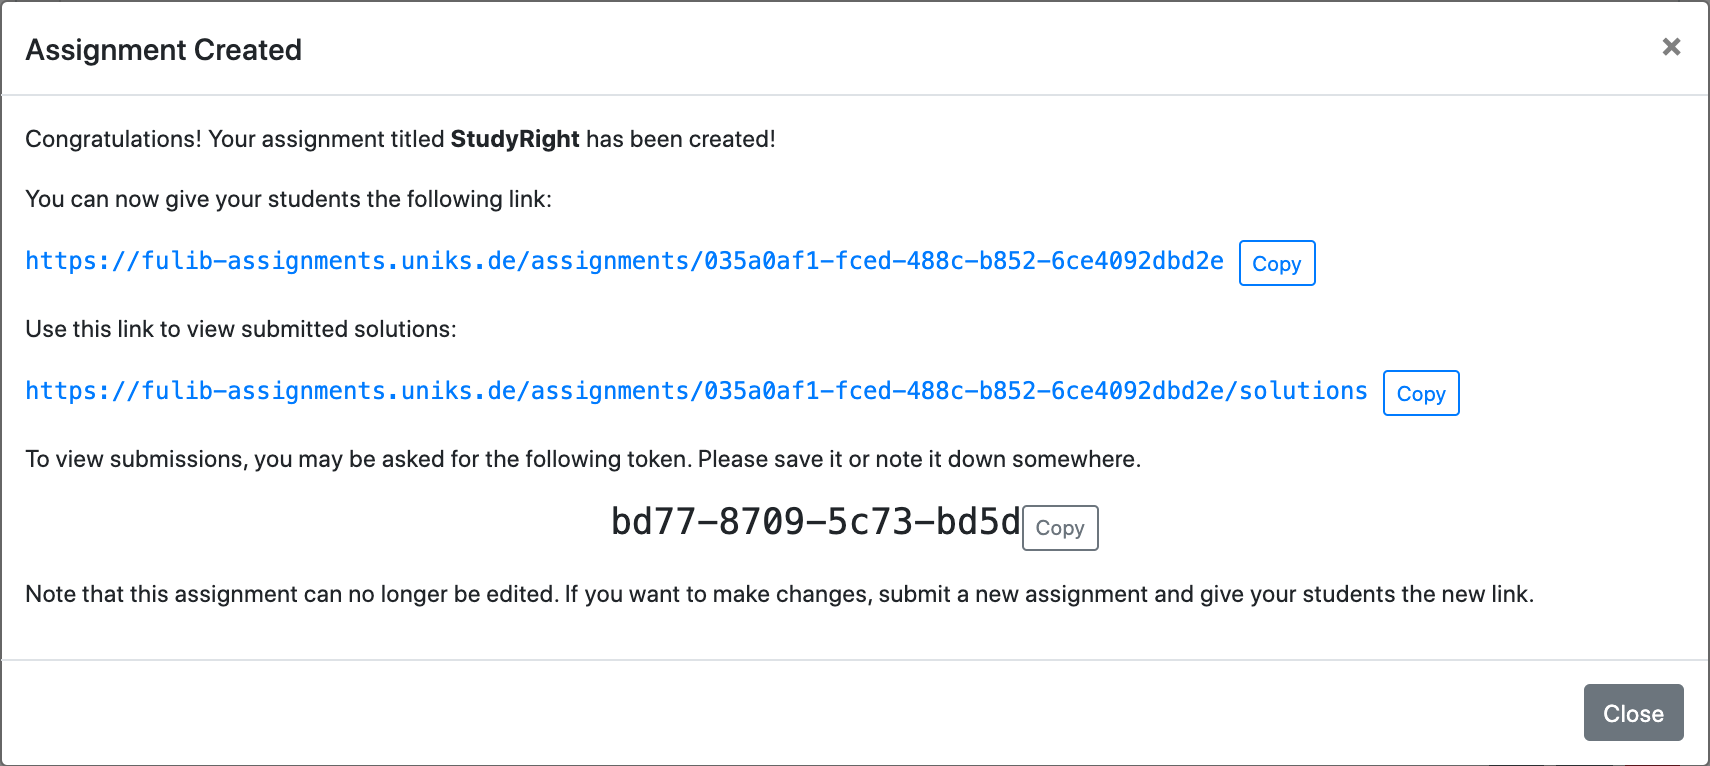
\includegraphics[width=\textwidth]{chapter/fulib.org/img/create-assignment-success.png}
    \caption{Fenster nach Anlegen eines Assignments}
    \label{fig:create-assignment-success}
\end{figure}

Der erste Link ist dafür vorgesehen, ihn an die Studierenden weiterzuleiten.
Öffnen sie diesen, zeigt sich die Seite, in der ihre Lösung des Assignments erstellt und abgegeben werden kann.
Dieser Vorgang ist Thema des nächsten Unterabschnitts.
Der zweite Link ist für den Kursleiter und die Korrekteure, da darunter eine Liste aller abgegebenen Lösungen zu finden ist.
Um darauf zugreifen zu können, wird das gezeigte Token benötigt.
Dieses muss vom Kursleiter an die Korrekteure weitergeleitet werden.
Ohne das Token-System könnten Studierende die Lösungen von Anderen einsehen und übernehmen.

Assignments sind nach dem Einreichen nicht mehr veränderbar.
Dies ist gewünscht, da das nachträgliche Verändern von Assignments, die schon von Studierenden bearbeitet wurden, für diese nachteilhaft sein kann.
Wird im Nachhinein ein Fehler in der Aufgabenstellung erkannt, kann das gleiche Assignment erneut eingereicht werden.
Dabei werden neue Links und Token generiert, die wieder entsprechend geteilt werden müssen.

Wählt man im Footer Assignments > My Assignments aus, gelangt man zur Übersicht der eigenen Assignments.
Abbildung~\ref{fig:my-assignments} zeigt, wie diese Seite aussehen kann.
Zu eigenen Assignments zählen diejenigen, deren Token im Browser gespeichert ist.
Dies umfasst einerseits die eigens erstellten Assignments, andererseits diejenigen, deren Lösungsliste bereits geöffnet und mit dem Token freigeschaltet wurde.
Diese Liste kann nützlich sein, wenn ein Link nicht mehr auffindbar ist.
Ein Klick auf einen Eintrag der Liste leitet auf die Liste mit Lösungen für das jeweilige Assignment weiter.

\begin{figure}
    \centering
    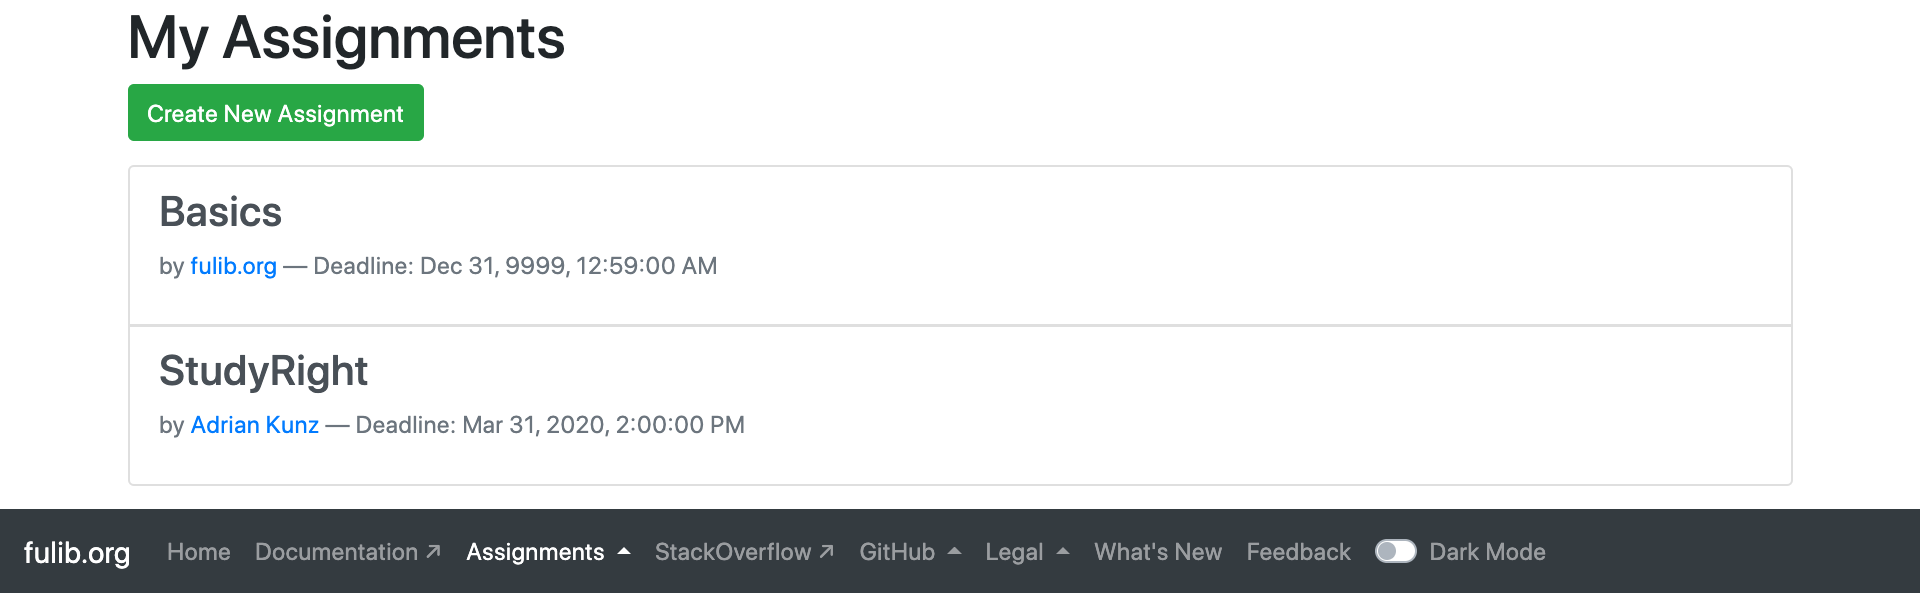
\includegraphics[width=\textwidth]{chapter/fulib.org/img/my-assignments.png}
    \caption{Liste der eigenen Assignments}
    \label{fig:my-assignments}
\end{figure}

\subsection{Lösen}\label{subsec:solution}

Studierende können ein Assignment lösen, indem sie dessen Link besuchen.
Daraufhin wird die in Abbildung~\ref{fig:assignment-solve} dargestellt Seite angezeigt.
Diese enthält alle beim Erstellen angegebenen Eckdaten, sowie die Beschreibung und Task-Liste des Assignments.
Darunter befindet sich der Editor für die Lösung.
In Abbildung~\ref{fig:assignment-solve} enthält dieser bereits die vom Ersteller vorgegebene Lösungsvorlage als Hilfe zum Einstieg.

\begin{figure}
    \centering
    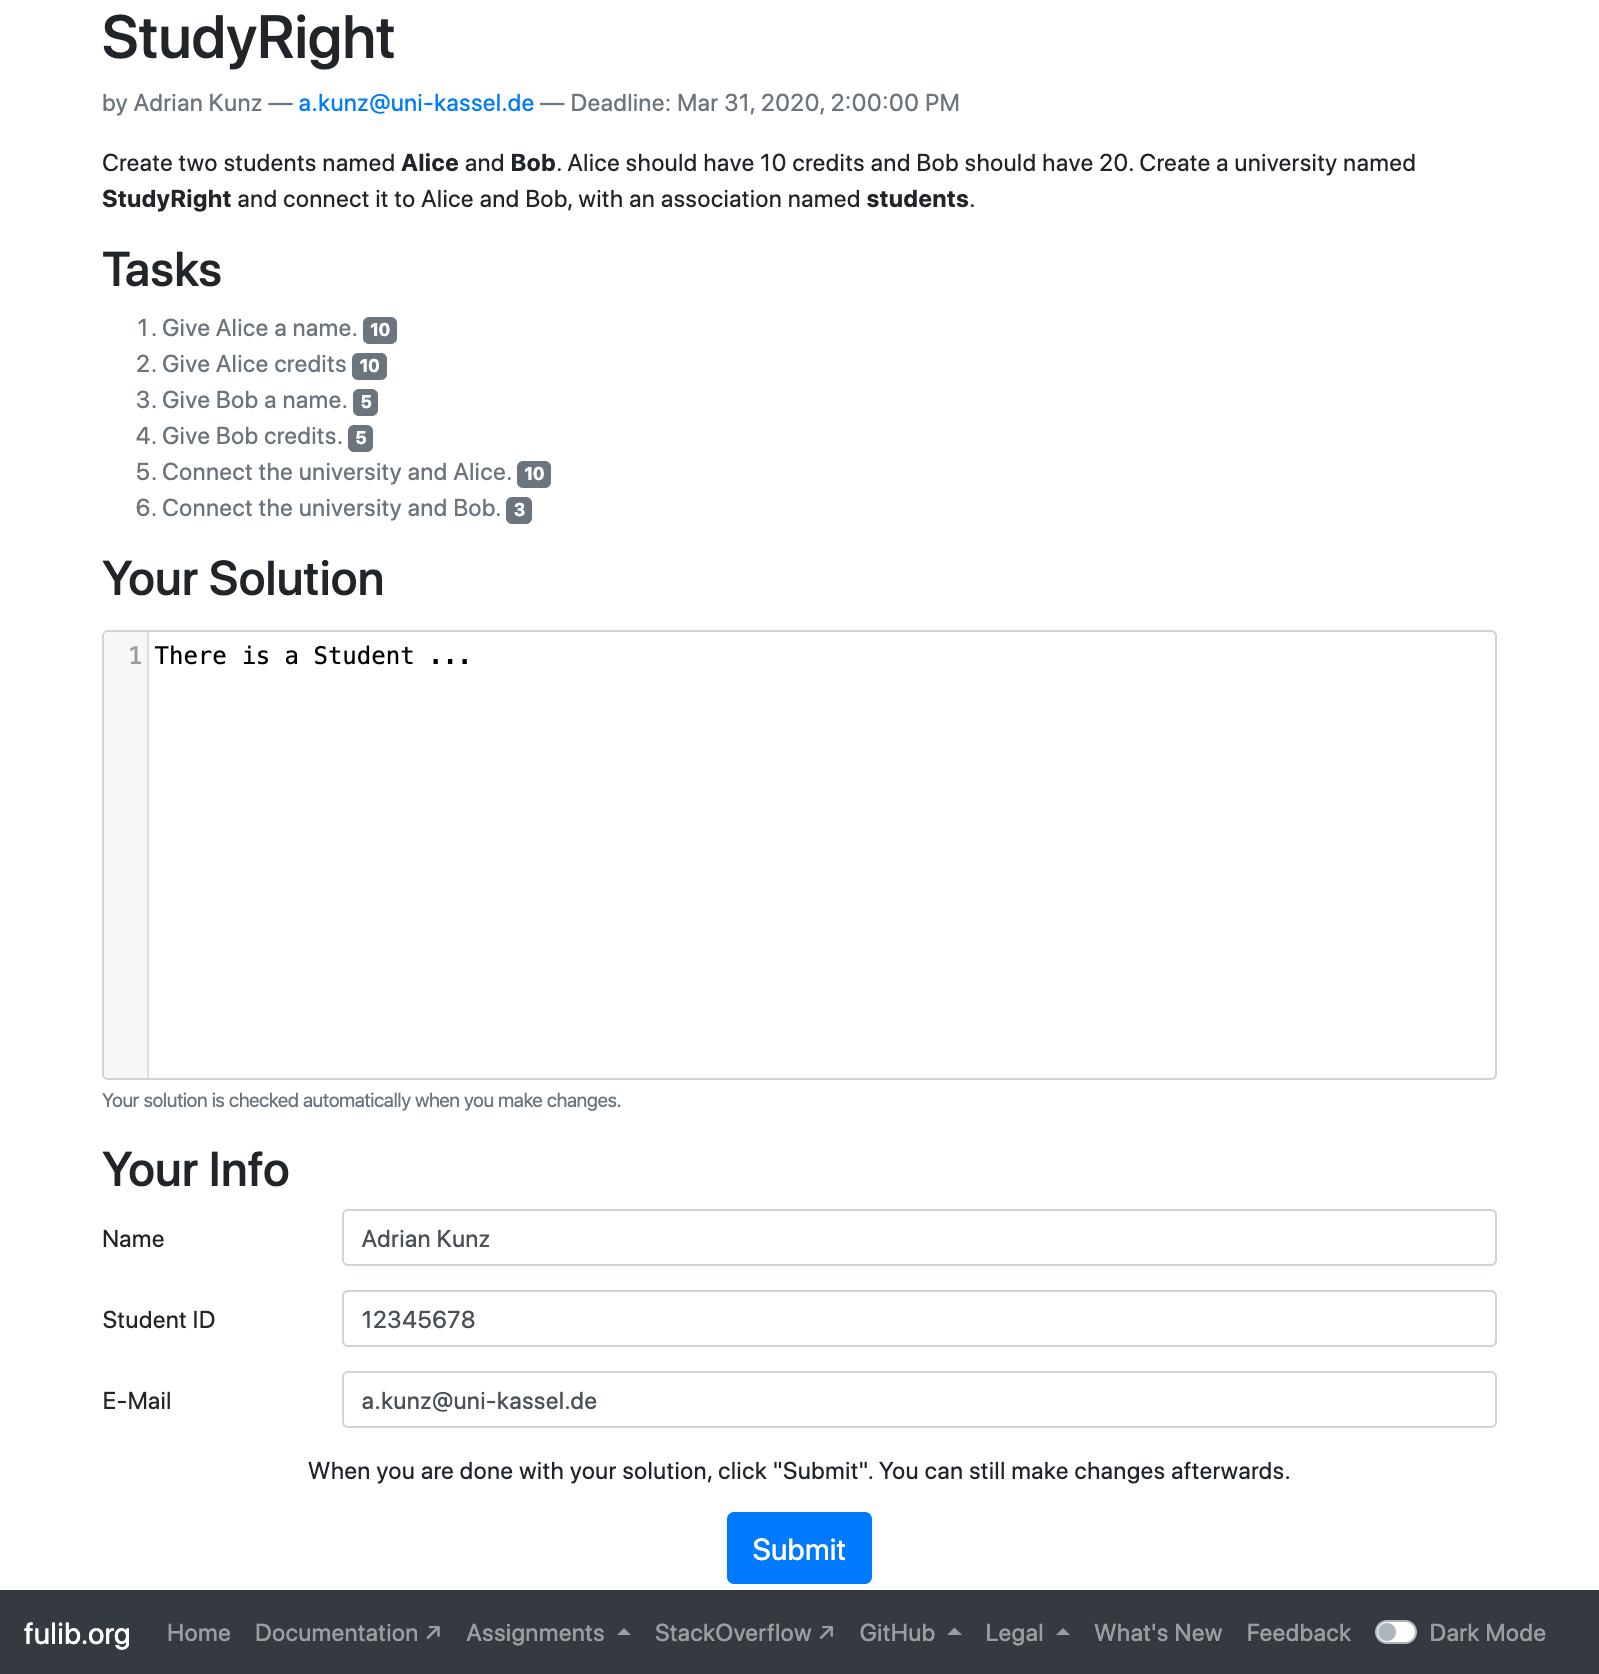
\includegraphics[width=\textwidth]{chapter/fulib.org/img/assignment-solve.png}
    \caption{Lösungsseite für ein Assignment}
    \label{fig:assignment-solve}
\end{figure}

Sobald man das Scenario im Editor bearbeitet, beginnt die automatische Prüfung anhand der Tasks.
Dabei werden erfüllte Tasks grün und nicht erfüllte Tasks rot markiert.
Auch die erreichte Punktzahl wird ermittelt und angezeigt.
Bei nicht erfüllten Tasks lässt sich mit ``View Output'' die Ausgabe des Scenario-Compilers anzeigen, die auf die Fehlerursache hinweist.
Abbildung~\ref{fig:solve-tasks} zeigt, wie dies bei einer Teillösung aussehen kann.
Der Studierende kann dann seine Lösung anpassen, um alle Tasks zu erfüllen.
Es ist jedoch auch möglich, eine teilweise oder vollständig fehlerhafte Lösung abzugeben.

\begin{figure}
    \centering
    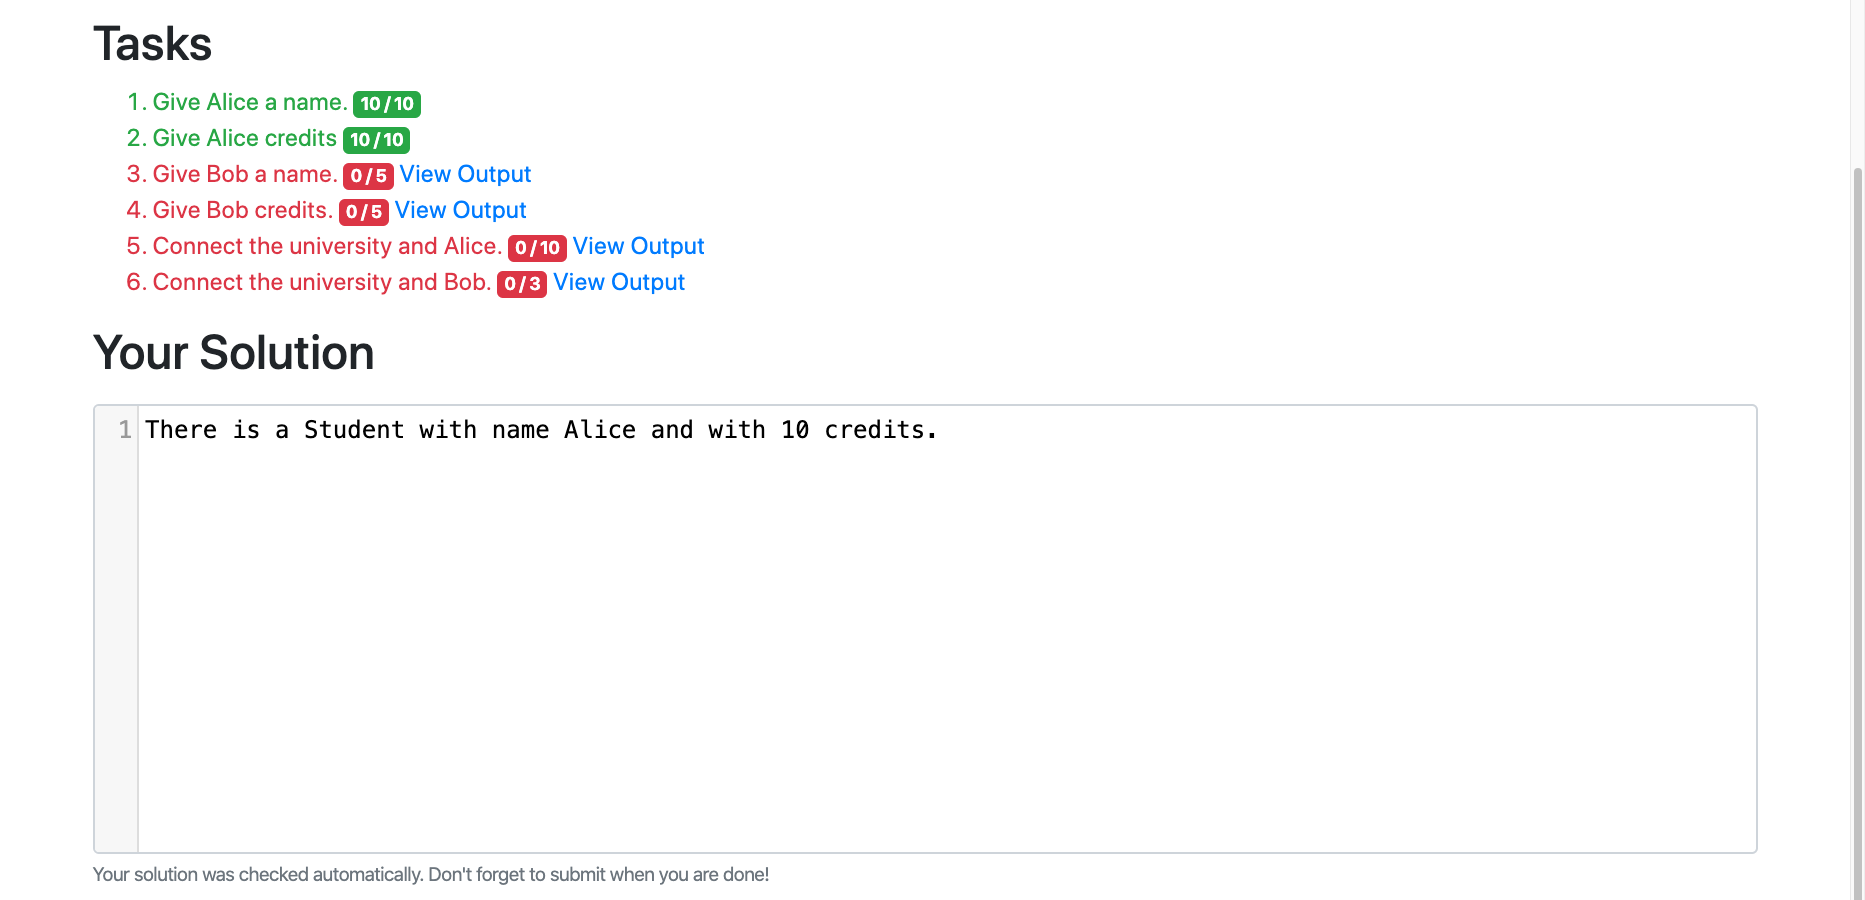
\includegraphics[width=\textwidth]{chapter/fulib.org/img/solve-tasks.png}
    \caption{Erfüllte und unerfüllte Tasks}
    \label{fig:solve-tasks}
\end{figure}

Um die Lösung abzugeben, muss der Studierende zunächst Namen, Matrikelnummer und E-Mail-Adresse angeben.
Daraufhin kann mit ``Submit'' die Lösung eingereicht werden.
Dies öffnet das in Abbildung~\ref{fig:solution-submitted} dargestellte Fenster.

\begin{figure}
    \centering
    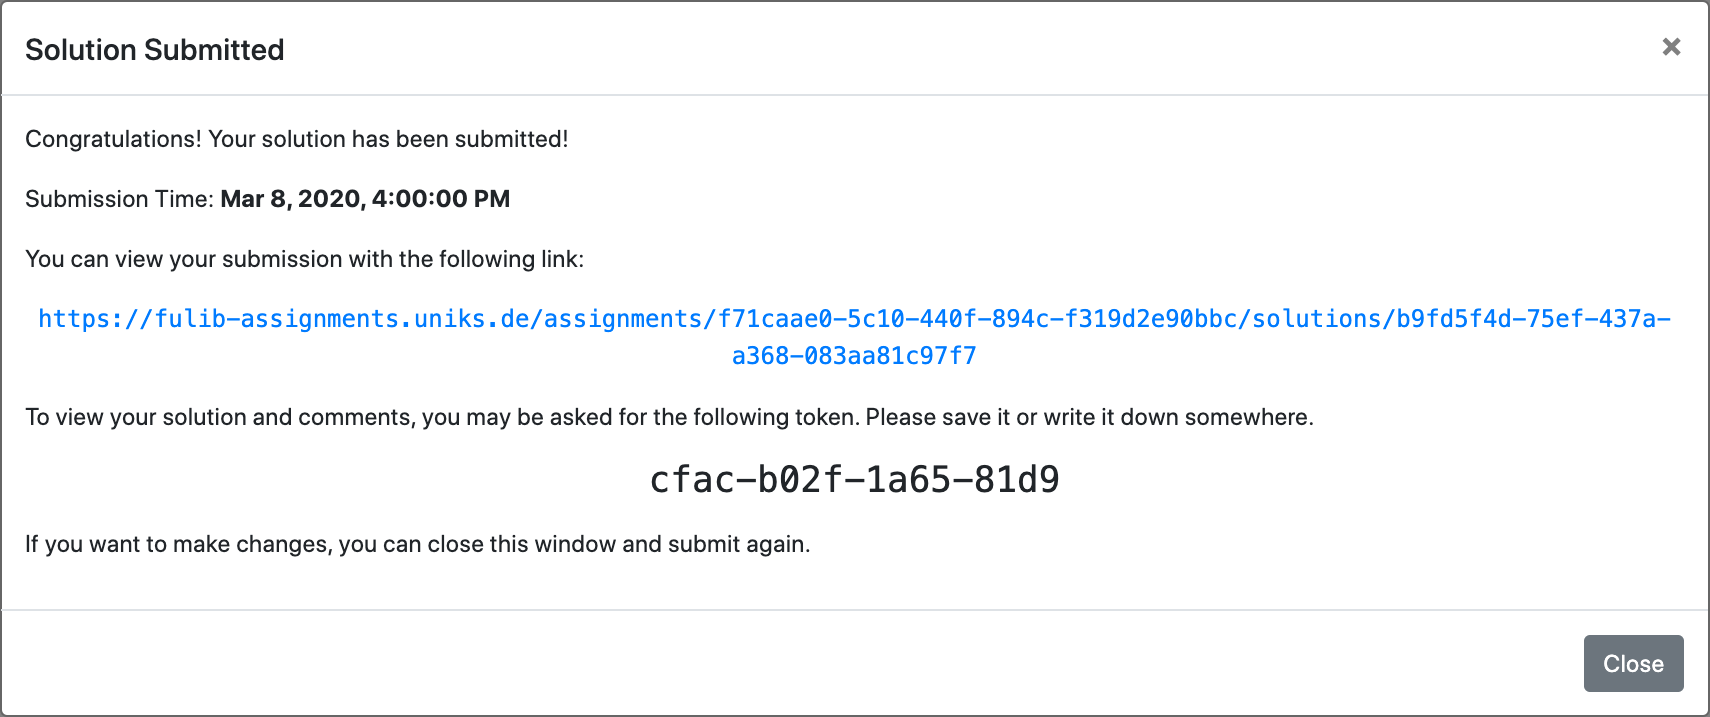
\includegraphics[width=\textwidth]{chapter/fulib.org/img/solution-submitted.png}
    \caption{Fenster nach Einreichen einer Lösung}
    \label{fig:solution-submitted}
\end{figure}

Auch für Lösungen wird ein Link und ein Token generiert.
Der Link dient dazu, die Lösung sowie deren Bewertung später einsehen zu können.
Dies ist aus Sicherheitsgründen nur mit dem Token möglich, das zwar im Browser gespeichert wird, jedoch beim Öffnen der Lösungsseite mit einem anderen Gerät eingegeben werden muss.

Nach der Abgabe kann der Lösungsentwurf weiter bearbeitet werden.
Dazu muss lediglich das Bestätigungsfenster geschlossen werden.
Durch erneutes Betätigen von ``Submit'' wird die neue Lösung eingereicht;
die alte Abgabe bleibt jedoch unverändert und weiterhin einsehbar.
Auch bei einem späteren Besuch der Seite bleiben sämtliche Eingaben bestehen, da sie im Browser gespeichert werden.
Dadurch kann an einer angefangen Lösung bedenkenlos später weitergearbeitet werden, ohne sie zwischenzeitlich einreichen zu müssen.

Studierende können ihre abgegebenen Lösungen einsehen, indem sie die Seite unter Assignments > My Solutions im Footer öffnen.
Dort finden sie sämtliche eingereichte Versionen nach Assignment gruppiert.
Abbildung~\ref{fig:my-solutions} zeigt, wie dies aussehen kann.
Der Button ``Edit'' erlaubt die Bearbeitung und erneute Abgabe einer Lösung.
Genauer öffnet er nur die Bearbeitungsseite des Assignments, wo die zuletzt im Browser gespeicherte Lösung angezeigt wird.
Diese kann von der zuletzt abgegebenen Version abweichen, wenn Änderungen vorgenommen aber nicht eingereicht wurden.

\begin{figure}
    \centering
    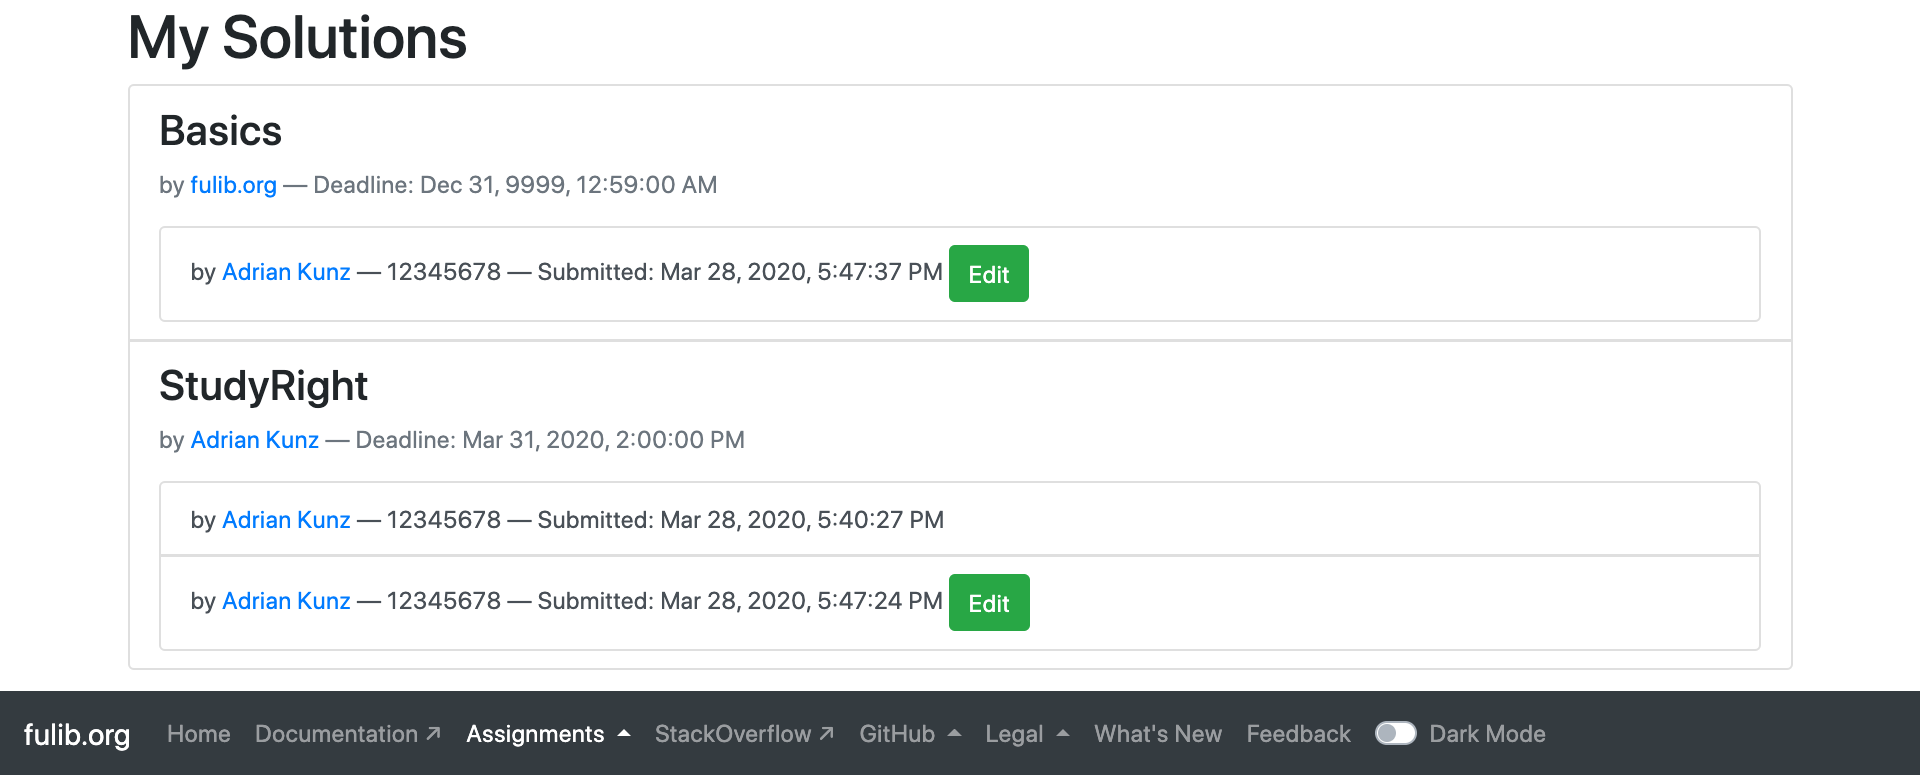
\includegraphics[width=\textwidth]{chapter/fulib.org/img/my-solutions.png}
    \caption{Liste der abgegebenen Lösungen}
    \label{fig:my-solutions}
\end{figure}

\subsection{Korrigieren}\label{subsec:correcting}

Einstiegspunkt für die Korrektur ist die Seite, auf der abgegebene Lösungen für ein Assignment einsehbar sind.
Diese ist unter dem zweiten Link erreichbar, der nach Anlegen eines Assignments erzeugt wurde.
Der Kursleiter kann diesen an die Korrekteure zusammen mit dem Token weiterleiten.
Beim ersten Besuch des Links muss letzteres angebeben werden, um die Lösungen anzuzeigen.
Daraufhin zeigt sich die Tabelle, die in Abbildung~\ref{fig:solution-table} zu sehen ist.

\begin{figure}
    \centering
    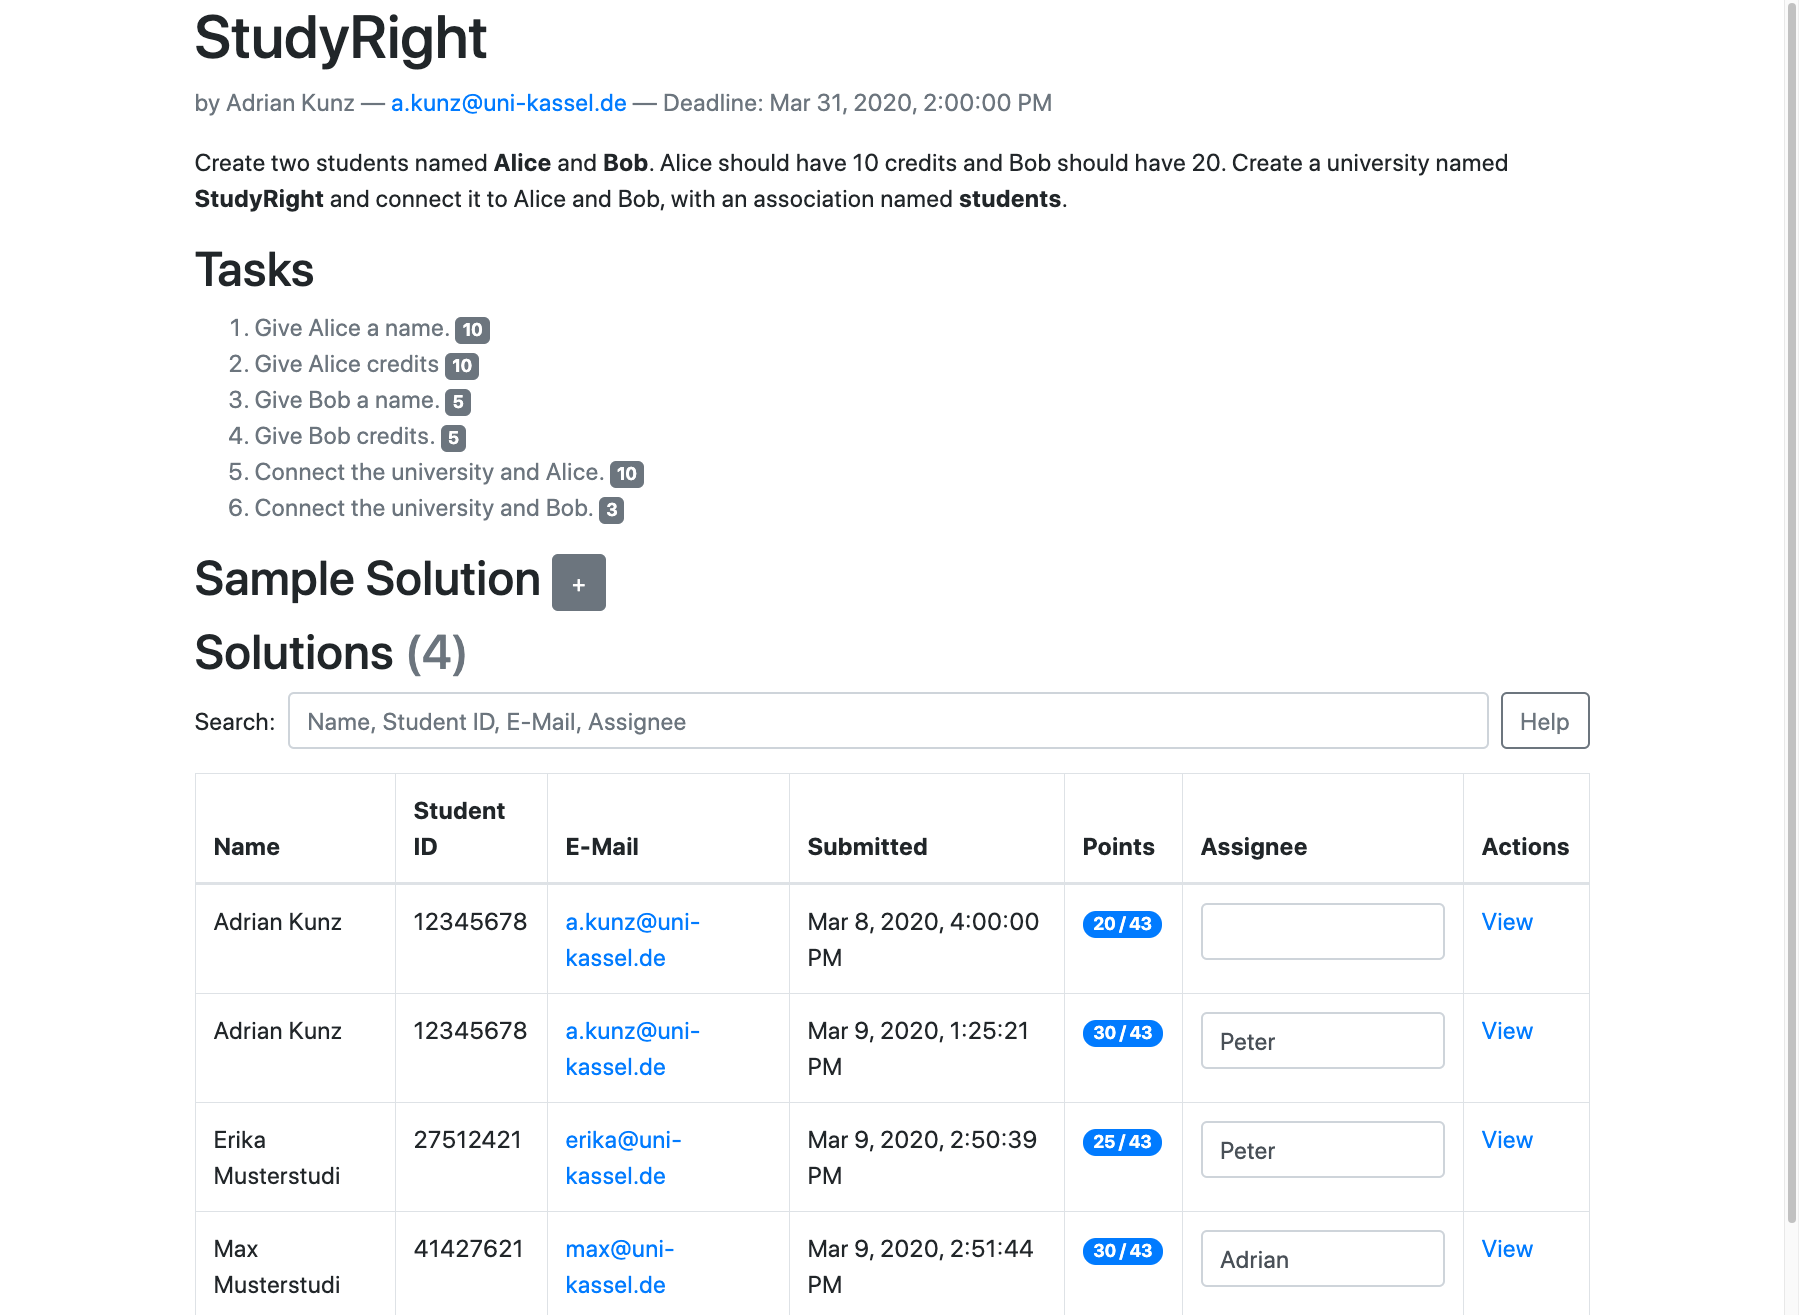
\includegraphics[width=\textwidth]{chapter/fulib.org/img/solution-table.png}
    \caption{Tabelle der eingereichten Lösungen für ein Assignment}
    \label{fig:solution-table}
\end{figure}

Über der Tabelle befindet sich eine Übersicht der Aufgabenstellung inklusive Eckdaten, Beschreibung, Tasks und eventueller Musterlösung.
Dies vereinfacht die Korrektur, da keine separate Seite geöffnet werden muss, um die Anforderungen einzusehen.
Das Suchfeld erlaubt es, die angezeigten Lösungen einzuschränken.
Dies ist sowohl als Freitextsuche über alle Spalten als auch für bestimmte Spalten möglich.
So lässt sich beispielsweise mit \code{assignee:Peter} nach allen Lösungen suchen, die dem Korrekteur \code{Peter} zugewiesen sind.
Die Zuweisung erfolgt durch Ändern des Eingabefelds unter ``Assignee'' und wird sofort übernommen.
In der Regel kann der Kursleiter diese Zuordnung durchführen, woraufhin die Korrekteure nach ihnen zugewiesenen Lösungen suchen können.

Die Tabelle gibt zunächst eine Übersicht über die Randangaben der Lösung.
Dazu gehören neben den Angaben zum Studierenden auch das Abgabedatum sowie die erreichte Punktzahl.
Nach der Deadline abgegebene Lösungen werden rot hervorgehoben.
Durch Klicken auf ``View'' gelangt man zur Detailseite der Lösung, die in Abbildung~\ref{fig:solution} dargestellt ist.

\begin{figure}
    \centering
    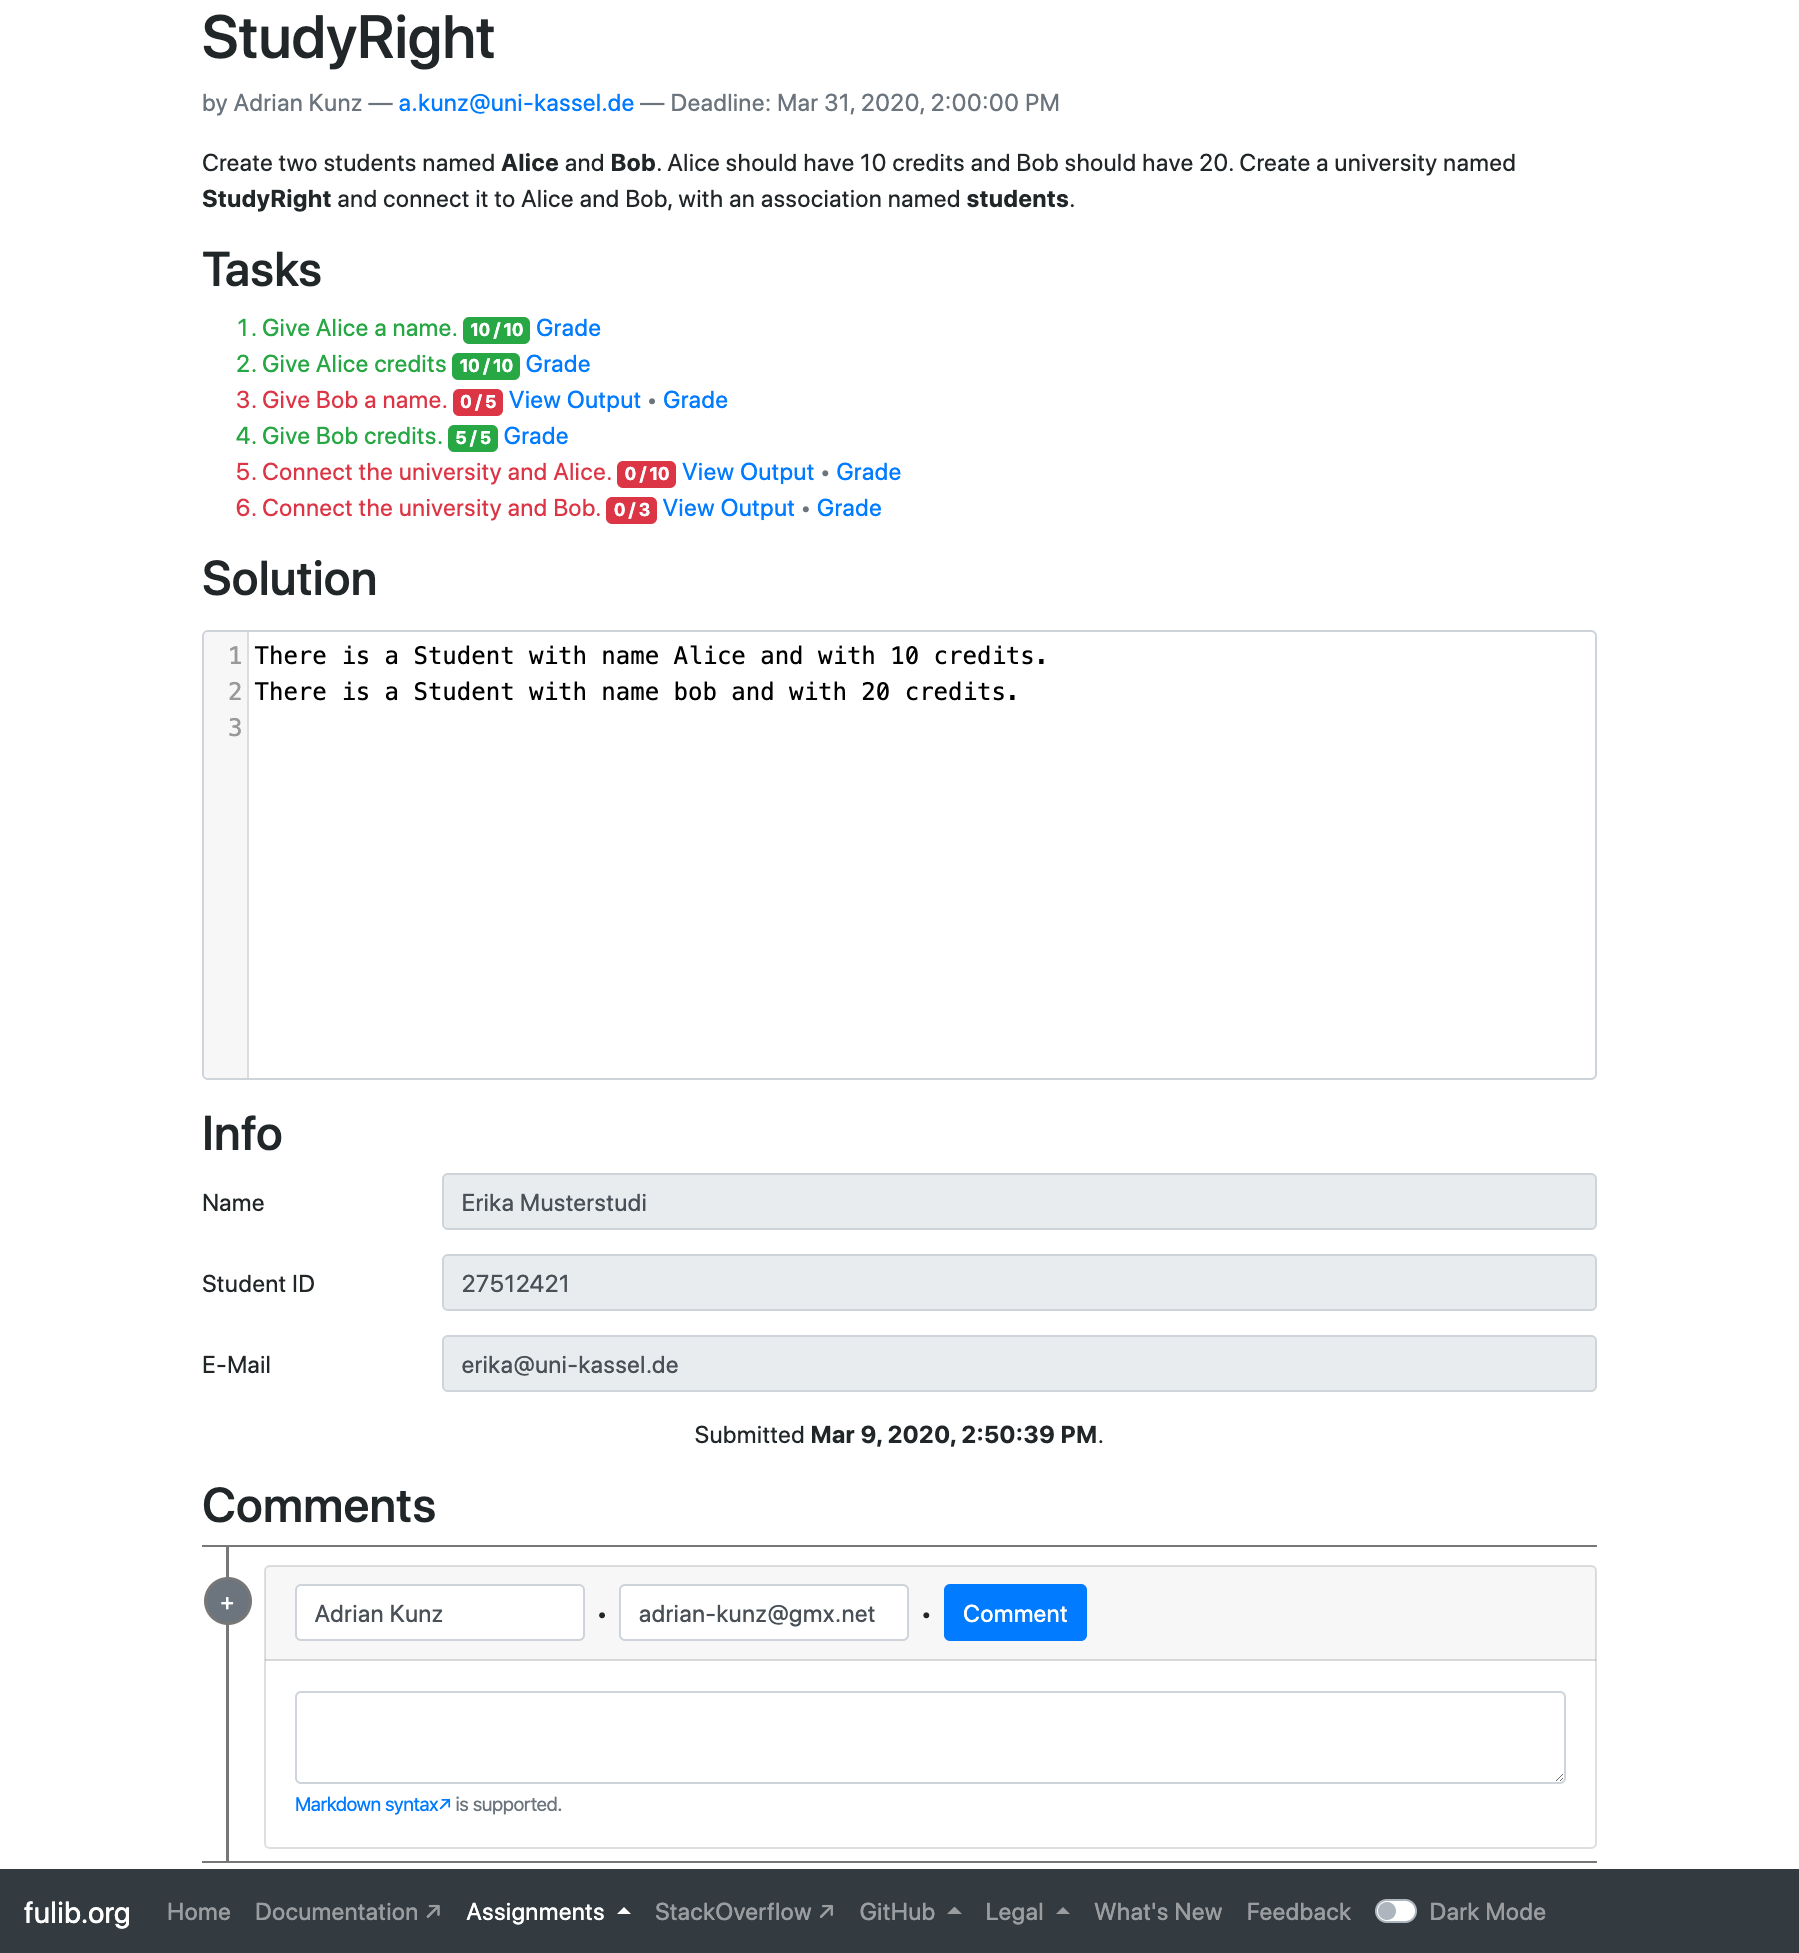
\includegraphics[width=\textwidth]{chapter/fulib.org/img/solution.png}
    \caption{Ansicht einer abgegebenen Lösung}
    \label{fig:solution}
\end{figure}

Hier wird erneut die Aufgabenstellung angezeigt.
Die Task-Liste zeigt die erreichte Punktzahl, die mittels ``Grade'' durch den Korrekteur angepasst werden kann.
Dabei muss die zu vergebende Punktzahl, ein kurzer Kommentar und der eigene Name angegeben werden.
In der Historie werden alle Änderungen der Bewertung aufgelistet.
Auch Studierende können diese einsehen, jedoch nicht verändern, da dafür das Token des Assignments benötigt wird.
Abbildung~\ref{fig:grade-popover} zeigt das Fenster der Bewertung eines Tasks.
Aufgrund der Vergabe von Teilpunkten wurde der entsprechende Task gelb markiert, was bei der automatischen Bewertung nicht möglich ist.

\begin{figure}
    \centering
    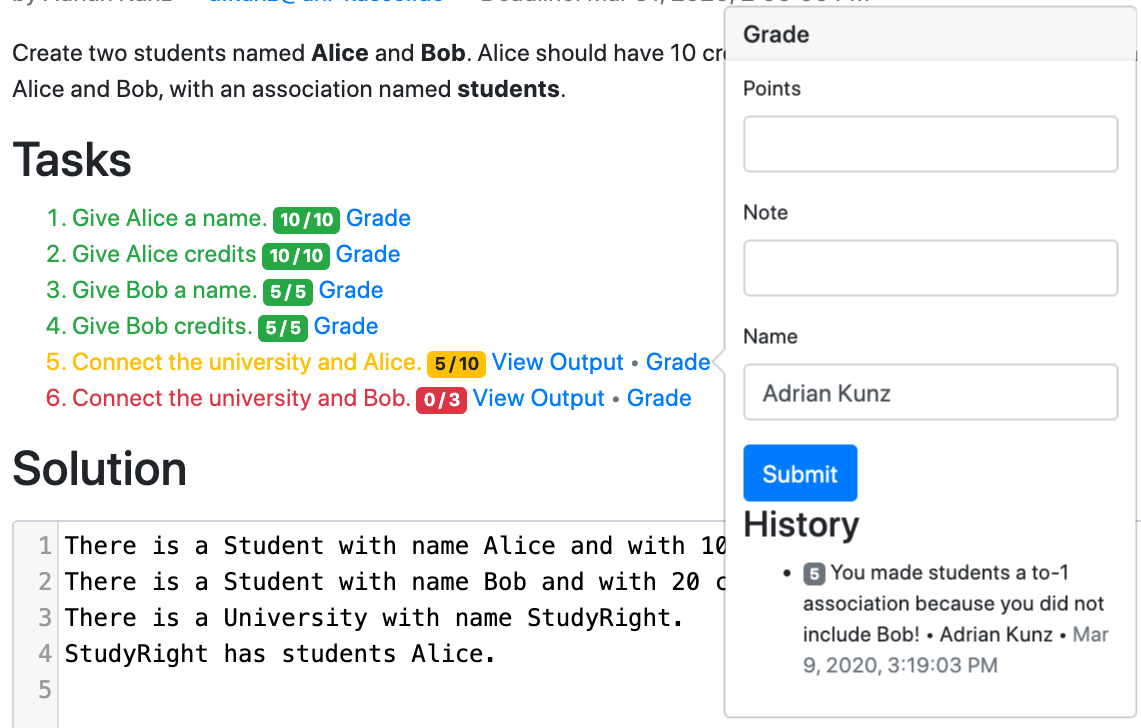
\includegraphics[width=0.5\textwidth]{chapter/fulib.org/img/grade-popover.png}
    \caption{Fenster zur Bewertung eines Tasks}
    \label{fig:grade-popover}
\end{figure}

Am unteren Ende der Seite befindet sich der Kommentarbereich.
Hier können Studierende und Korrekteure Fragen, Antworten und Anmerkungen zur Bewertung hinterlassen.
Ist das Token des Assignments vorhanden und ein Kommentar wird erstellt, wird dieser mit einem Häkchen hinter dem Namen hervorgehoben.
Dies verhindert, dass Studierende den Kursleiter oder einen Korrekteur imitieren können, indem sie deren Namen angeben.

\subsection{Kurse}\label{subsec:courses}

Kurse sind Sammlungen von Assignments, die eine feste Reihenfolge vorgeben.
Sie ermöglichen die Vergabe von mehreren Aufgabenstellungen, die inhaltlich zusammengehören und aufeinander aufbauen können.
So ist es beispielsweise möglich, einen unbeaufsichtigten, von einer Vorlesung unabhängigen Kurs zu erstellen, mit dem die Scenario-Sprache erlernt werden kann.
Interessierte können diesen aufrufen und selbstständig Assignments bearbeiten, die nicht von Korrekteuren bewertet werden.

Kurse werden erstellt, indem im Footer Assignments > Create Course ausgewählt wird.
Dies öffnet die in Abbildung~\ref{fig:create-course} gezeigte Seite.

\begin{figure}
    \centering
    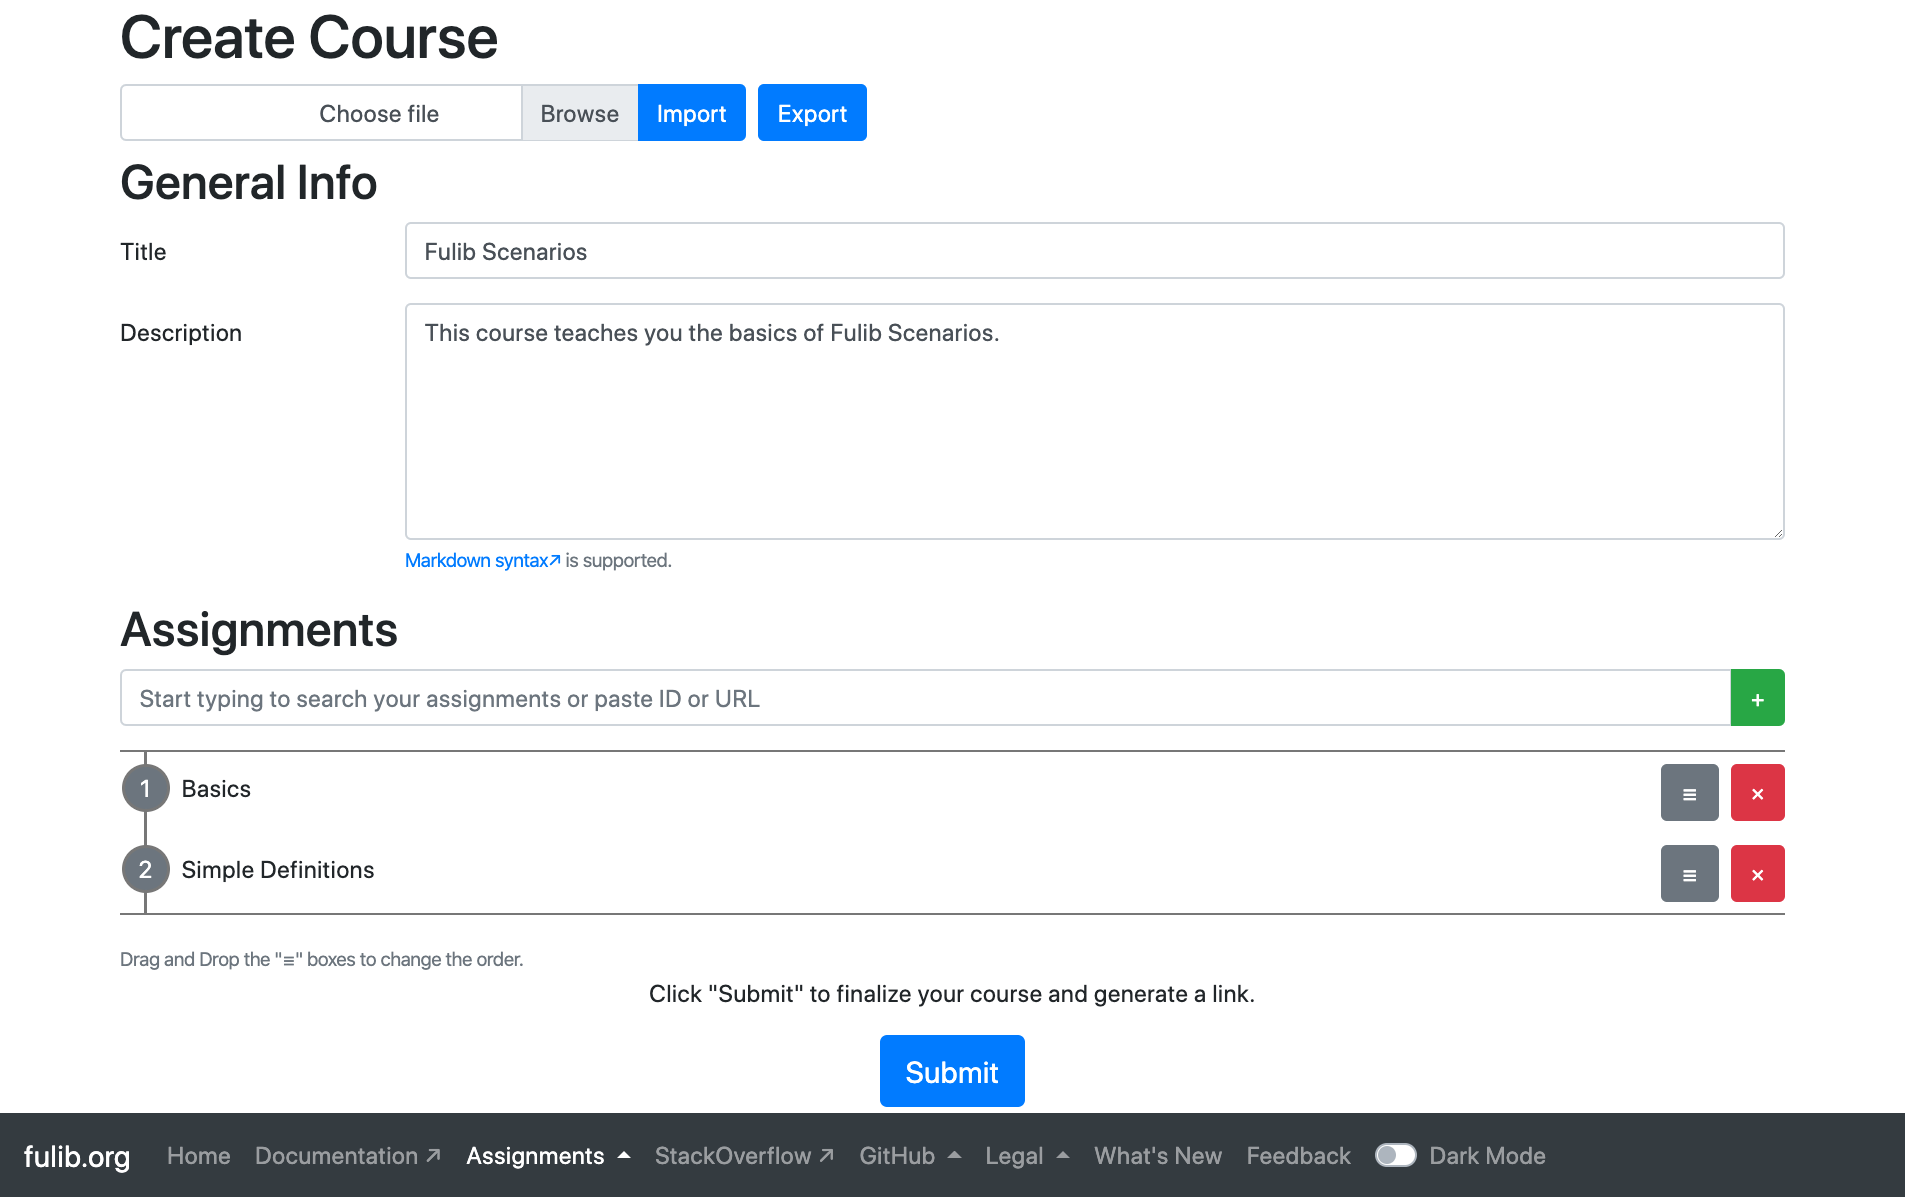
\includegraphics[width=\textwidth]{chapter/fulib.org/img/create-course.png}
    \caption{Formular zum Erstellen eines Kurses}
    \label{fig:create-course}
\end{figure}

Ein Kurs benötigt neben den zugehörigen Assignments einen Titel und eine Beschreibung.
Assignments müssen im Vorhinein mit dem in Unterabschnitt~\ref{subsec:creation} erläuterten Formular erstellt werden.
Diese lassen sich dann mit dem dafür vorgesehenen Feld dem Kurs hinzufügen.
Alternativ können beliebige Assignments von anderen Erstellern eingebunden werden, solange der zugehörige Link bekannt ist.
Die dabei entstehenden Liste erlaubt das Entfernen der hinzugefügten Assignments sowie das Ändern ihrer Reihenfolge.
Dafür werden die gleichen Steuerelemente wie in der Task-Liste beim Anlegen eines Assignments verwendet.
Zum Erstellen genügt nach Ausfüllen des Formulars ein Klick auf den Button ``Submit''.
Dabei wird ein Link generiert, unter dem der Kurs abrufbar ist.
Abbildung~\ref{fig:course-view} zeigt die Seite, die damit aufgerufen wird.

\begin{figure}
    \centering
    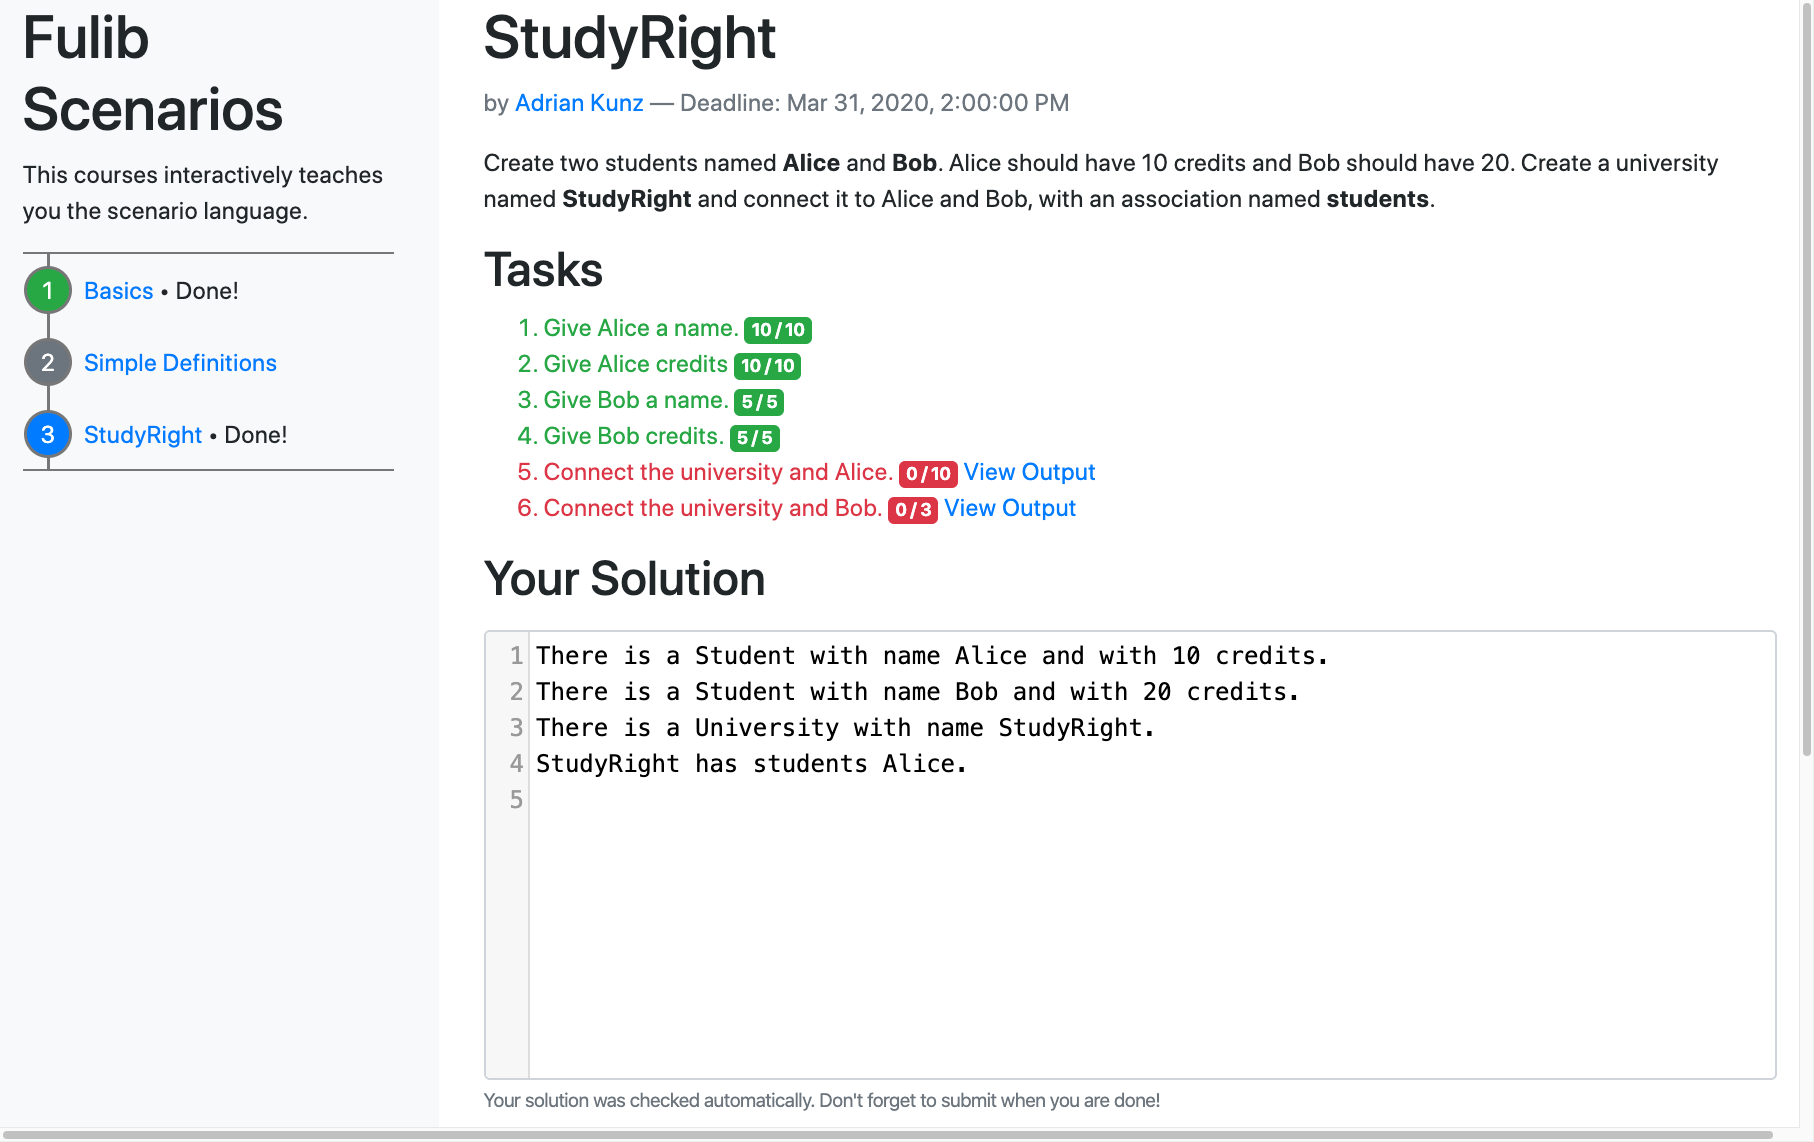
\includegraphics[width=\textwidth]{chapter/fulib.org/img/course-view.png}
    \caption{Kurs-Ansicht}
    \label{fig:course-view}
\end{figure}

Die Bearbeitung eines Assignments in einem Kurs unterscheidet sich nur geringfügig von der eines alleinstehenden Assignments.
Am linken Bildschirmrand kommt eine Seitenleiste hinzu, die Titel, Beschreibung und Verlauf des Kurses anzeigt.
Darin werden das aktuell angezeigte sowie bereits bearbeitete Assignments hervorgehoben.
Die Assignments eines Kurses können in beliebiger Reihenfolge bearbeitet werden.
Grund dafür ist, dass sie auch außerhalb des Kurses beliebig abruf- und bearbeitbar sind und somit die Einschränkung leicht umgangen werden könnte.
In der Regel ist es jedoch sinnvoll, sich an den vorgegebenen Ablauf zu halten.
Bearbeitet man ein Assignment als Teil eines Kurses und reicht eine Lösung ein, verändert sich das Bestätigungsfenster der Abgabe.
In diesem kommt ein Button hinzu, der das Fortschreiten zum nächsten Assignment im Kurs erlaubt.

\subsection{Pattern Matching in Assignments}\label{subsec:assignment-pattern-matching}

Die vorherigen Beispiele für Assignments verwendeten nur einfache Funktionalität der Scenario-Sprache zum Prüfen von Bedingungen.
Es wird nun anhand der in Kapitel~\ref{ch:pattern-matching} vorgestellten Konzepte ein vollständiges Beispiel vorgestellt, dessen Aufgabe es sein soll, das im gleichen Kapitel erklärte Spiel zu modellieren.
Die Aufgabenstellung soll bewusst Freiheiten bei der Benennung von Klassen und Attributen erlauben;
lediglich die Struktur des zu erstellenden Modells wird vorgegeben.
Vorgaben werden durch die Tasks des Assignments gestellt, die nach Möglichkeit unabhängig voneinander sein sollen.
Dadurch soll es möglich sein, Teilpunkte zu erhalten.

Zu einem vollständigen Assignment gehören zunächst die Eckdaten.
Der Titel des Assignments kann beispielsweise ``Game Model'' lauten.
Name und E-Mail sind in diesem Fall nicht relevant, ebenso wenig die Deadline.
Als Beschreibung wäre etwa folgender Text vorstellbar:

\begin{quote}
    This assignment is about modelling a simple game with multiple players.
    Each player has one or more houses, each of which has a number of units.
    The game has a score that must be beaten by at least one house.
    The player who owns that house is then declared the winner.

    Model the objects and relationships described below.
\end{quote}

Dieser Beispieltext ist bewusst kurz gehalten, da die eigentlichen Aufgaben in den Task-Beschreibungen zu finden sind.
Nachfolgend sind alle Tasks mit dem zugehörigen Verifizierungscode sowie einer möglichen Punktzahl aufgelistet.

\begin{itemize}
    \item \textbf{Create a game object and give it a minimum score of 50.} (5 Punkte)

    \begin{mdcodeblock}
        We match some object g where some attribute is 50.
    \end{mdcodeblock}

    \item \textbf{Create three players: Alice, Bob and Charlie.
    Set their name in an attribute.} (15 Punkte)

    \begin{mdcodeblock}
        We match:
        - some object alice1 where some attribute matches '(?i)alice'
        - some object bob1 where some attribute matches '(?i)bob'
        - some object charlie1 where some attribute matches '(?i)charlie'.
    \end{mdcodeblock}

    \item \textbf{Link the players with the game.} (5 Punkte)

    \begin{mdcodeblock}
        We match:
        - some object alice1 where some attribute matches '(?i)alice' and with some link to g
        - some object bob1 where some attribute matches '(?i)bob' and with some link to g
        - some object charlie1 where some attribute matches '(?i)charlie' and with some link to g
        - some object g where some attribute is 50.
    \end{mdcodeblock}

    \item \textbf{Create four houses, with 30, 20, 40 and 60 units.} (10 Punkte)

    \begin{mdcodeblock}
        We match:
        - some object h1 where some attribute is 30
        - some object h2 where some attribute is 20
        - some object h3 where some attribute is 40
        - some object h4 where some attribute is 60.
    \end{mdcodeblock}

    \item \textbf{Link the first two houses with Alice, and the other two with Bob and Charlie.} (5 Punkte)

    \begin{mdcodeblock}
        We match:
        - some object h1 where some attribute is 30 and with some link to alice1
        - some object h2 where some attribute is 20 and with some link to alice1
        - some object h3 where some attribute is 40 and with some link to bob1
        - some object h4 where some attribute is 60 and with some link to charlie1
        - some object alice1 where some attribute matches '(?i)alice'
        - some object bob1 where some attribute matches '(?i)bob'
        - some object charlie1 where some attribute matches '(?i)charlie'.
    \end{mdcodeblock}
\end{itemize}

Eine Musterlösung könnte das folgende Scenario sein:

\begin{mdcodeblock}
    There is a Game with min-score 50.

    There is a Player with name Alice.
    There is a Player with name Bob.
    There is a Player with name Charlie.

    The game has players and is game of Alice, Bob and Charlie.

    There is a House with id a1 and with 30 units.
    There is a House with id a2 and with 20 units.
    There is a House with id b1 and with 40 units.
    There is a House with id c1 and with 60 units.

    Alice has houses and is player of a1 and a2.
    Bob has houses b1.
    Charlie has houses c1.
\end{mdcodeblock}

Dabei können die Klassennamen \code{Game}, \code{Player} und \code{House} sowie die Attribut-\ und Assoziationsnamen \code{min-score}, \code{name}, \code{players/game}, \code{units} und \code{houses/player} beliebig verändert werden, ohne dass die Lösung ihre Gültigkeit verliert.
Beim Schreiben der Lösung fällt auf, dass mit jedem Absatz ein weiterer Task erfüllt und damit grün markiert wird.
Lässt man den dritten oder den letzten Absatz aus, sind die Tasks 1, 2 und 4 noch immer erfüllt.
Dies wird durch die unabhängige Verifizierung erreicht.
So können Studierende, die beispielsweise nicht wissen, wie Assoziationen definiert werden, noch Teilpunkte auf das Aufgabenblatt erhalten, indem sie nur Objekte und Attribute anlegen.
Eine Teillösung, die diese beiden Aspekte einbezieht, könnte folgende sein:

\begin{mdcodeblock}
    There is the SimpleGame sg with score 50.

    There is the SimplePlayer p1 with name Alice.
    There is the SimplePlayer p2 with name Bob.
    There is the SimplePlayer p3 with name Charlie.

    There is the PlayerHouse p1h1 with 30 fighters.
    There is the PlayerHouse p1h2 with 20 fighters.
    There is the PlayerHouse p2h1 with 40 fighters.
    There is the PlayerHouse p3h1 with 60 fighters.
\end{mdcodeblock}

\section{Architektur}\label{sec:architecture}

Fulib.org verwendet eine einfache Architektur, bestehend aus Frontend, Backend und Datenbank.
Da es sich um eine Webanwendung handelt, wird das Frontend im Browser ausgeführt.
Öffnet man die Seite, werden die benötigten HTML-, JavaScript- und CSS-Dateien vom Backend heruntergeladen und im Browser angezeigt.
Aus Sicht des Backends sind dies statische Ressourcen.
Sämtlicher Datenaustausch in der Webanwendung geschieht dann über HTTP-Anfragen an das Backend.
Dabei wird JSON als Datenformat verwendet.
Für die persistente Datenspeicherung von Anfragelogs, Aufgabenblättern, Lösungen, Kursen und Kommentaren kommt eine Mongo-Datenbank~\cite{mongodb} zum Einsatz.
Die Kompilierung und Ausführung von Scenarios wird durch Anbinden des Scenario- und Java-Compilers sowie einer JUnit-Laufzeit bewerkstelligt.
Abbildung~\ref{fig:website-architecture} gibt einen Überblick über die verschiedenen Komponenten, die es der Webseite ermöglichen, ihre Funktionalität bereitzustellen.
Im folgenden Abschnitt wird näher erläutert, wie diese zusammenwirken.

\begin{figure}
    \centering
    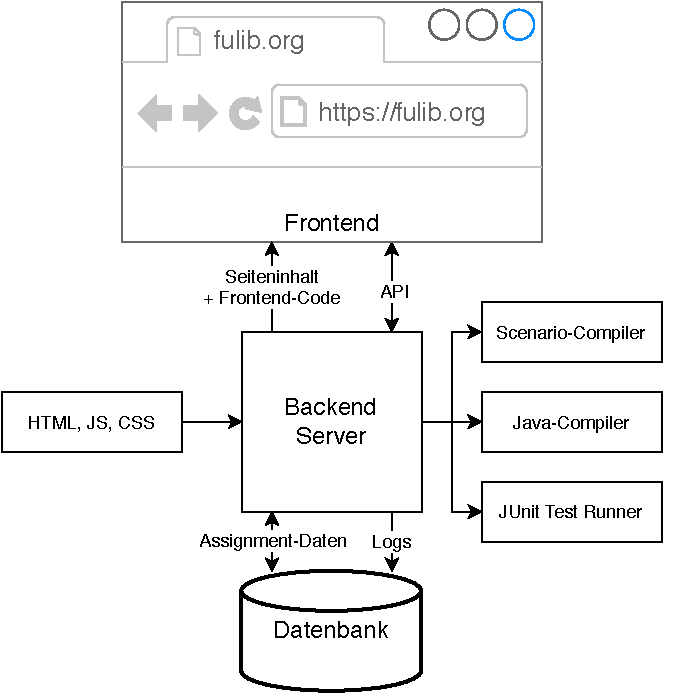
\includegraphics[width=0.5\textwidth]{chapter/fulib.org/img/architecture.pdf}
    \caption{Architektur von fulib.org}
    \label{fig:website-architecture}
\end{figure}

\subsection{Frontend}\label{subsec:frontend}

% Angular
Das Frontend von fulib.org ist mit dem Angular-Framework~\cite{angular} implementiert.
Dieses gibt eine Architektur vor, die Anwendungslogik (Services) von UI-Logik (Komponenten) trennt.
Services sind beispielsweise dafür zuständig, mit dem Backend Daten auszutauschen.
Mittels Dependency Injection lassen sich diese von Komponenten oder von anderen Services beziehen.
Die Komponenten befassen sich mit der Darstellung der Anwendung.
Sie bestehen aus einem HTML-Template, eigenem CSS und einer Klasse, die Daten mit Services kommuniziert und die Logik der Benutzeroberfläche implementiert.
Komponenten haben besonders als wiederverwendbare Elemente Bedeutung.
Sie ermöglichen es, gemeinsame Funktionalität zu verkapseln und an mehreren Stellen in der Anwendung zu verwenden.
Im Kontext der Assignments ist beispielsweise die Task-Liste eine Komponente, die auf mehreren Seiten zum Einsatz kommt.
Da Komponenten nur einmal implementiert werden und beliebig oft wiederverwendbar sind, kann die Oberfläche konsistent gehalten und Fehler vermieden werden.

% Bootstrap + Darkmode
Das Aussehen der Oberfläche von fulib.org basiert auf Bootstrap~4~\cite{bootstrap}.
Das CSS-Framework gibt vielen HTML-Elementen wie Buttons oder Eingabefeldern ein modernes Aussehen.
Ferner ermöglicht es die einfache Anordnung von Elementen, die sich an verschiedene Bildschirmgrößen anpassen kann.
Somit ist fulib.org ohne großen Entwicklungsaufwand auch auf Smartphones und anderen Mobilgeräten übersichtlich.
Bei dem im Footer einstellbaren Nachtmodus handelt es sich um Funktionalität, die von der Bootstrap-Darkmode-Bibliothek~\cite{bootstrap-darkmode} bereitgestellt wird.
Diese Eigenentwicklung passt die Farbgebung von Bootstrap so an, dass alle normalerweise weißen oder hellen Elemente in schwarz bzw.\ Grautönen erscheinen.
Dies schont bei dunkleren Lichtbedingungen das Auge.

% CodeMirror
Die Editorfenster für Scenarios und Java-Code sind mit der CodeMirror-Bibliothek~\cite{codemirror} implementiert.
Diese bietet einen Editor, der Syntaxhighlighting für viele Programmier- und Markupsprachen unterstützt.
Der Editor erlaubt die Anpassung der Farbgebung, was auf fulib.org beim Wechsel in den Nachtmodus zu beobachten ist.
Zudem unterstützt der Editor eine Reihe von Addons, die zusätzliche Funktionalität einbringen können.
Beispielsweise ermöglicht ein Lint-Addon die Hervorhebung von Fehlermeldungen im Editor.
Es ist geplant, diese im Scenario-Editor umzusetzen.

\subsection{Backend}\label{subsec:backend}

Beim Backend von fulib.org handelt es sich um einen einfachen HTTP-Server.
Dieser ist zustandslos, arbeitet also nach dem REST-Prinzip.
Dabei sind die Hauptaufgaben die Auslieferung des Frontends, die Ausführung von Scenarios sowie die Kommunikation mit der Datenbank im Kontext von Assignments.

% Frontend
Als Teil des Buildprozesses von fulib.org werden statische HTML-, JavaScript- und CSS-Dateien erzeugt, die das gesamte Frontend umfassen.
Diese werden vom Backend auf Anfrage eines Browsers unverändert an diesen übermittelt.
Anders als bei serverseitig generierten Webseiten hat dies den Vorteil, dass der Ressourcenaufwand des Servers sehr gering ist.
Auch lassen sich die statischen Ressourcen sehr gut zwischenspeichern, beispielsweise in einem Cache oder im Browser.
Dadurch können, mit Ausnahme vom ersten Besuch der Seite, die Ladezeiten erheblich verkürzt werden.
Der Aufwand steigt jedoch auf Client- bzw.\ Browserseite, der nach Herunterladen der statischen Dateien das JavaScript ausführen muss, um den Webseiteninhalt aufzubauen.
Dieser Vorgang kann bei weniger leistungsfähigen Geräten für längere Verzögerungen sorgen.
Ebenso ist zu beachten, dass fulib.org bei deaktiviertem oder nicht unterstützem JavaScript zwar aufrufbar, jedoch nicht verwendbar ist.
In diesem Fall wird eine Meldung in Form eines Banners angezeigt, die den Benutzer zur Aktivierung auffordert und dafür Hilfe anbietet.

% Scenario Compile and Run
Die Ausführung der Scenarios delegiert das Backend an die drei zuständigen Tools.
Nacheinander werden Scenario- und Java-Compiler sowie der JUnit-Testprozess ausgeführt.
Der Server schreibt zunächst den über die API empfangenen Text in eine Datei in einem temporären Ordner.
Daraufhin wird der Scenario-Compiler in diesem Ordner ausgeführt, der die Java-Dateien sowie das Klassendiagramm generiert.
Mit dem Java Compiler wird der Java-Code dann kompiliert und die entstehenden Klassen dynamisch geladen.
Das JUnit-Framework bietet eine Schnittstelle zum Ausführen der Test-Klassen an, wodurch das Testergebnis sowie die Objektdiagramme entstehen.
Die Ausgaben der drei Tools werden dabei protokolliert, da diese Teil der Antwort werden.
Der temporäre Ordner wird anschließend nach Diagramm- und Java-Dateien durchsucht.
Diagramme werden unter Anwendung einer geeigneten Codierung in die API-Antwort übernommen.
Aus Java-Dateien werden relevante Methodenrümpfe durch einen einfachen Parser extrahiert.

% Database
Die Kommunikation mit der Datenbank ist besonders bei Assignments und verwandter Funktionalität relevant.
Alle dafür zuständigen Endpunkte lesen entweder aus der Datenbank oder erzeugen darin neue Datensätze.
Beim Anlegen ist das Anfrageformat stets JSON, das der Server zunächst in sein eigenes Datenmodell konvertiert.
Dieses wird beim Speichern in der Datenbank in deren natives Format konvertiert.
Umgekehrt ist es bei Leseanfragen, bei denen der Server Anfragen an die Datenbank stellt, deren Ergebnis in sein Datenmodell konvertiert und dies als JSON in der Antwort zurückgibt.
Das Backend ist bei sämtlichen Anfragen für die Prüfung von Tokens zur Autorisierung zuständig, wobei sichergestellt wird, dass keine Daten bei unbefugten Anfragen preisgegeben werden.
Diese Prüfung wird insbesondere nicht im Frontend durchgeführt, da sonst ein Angreifer manuell die Server-API ansprechen und ausnutzen könnte.


	\chapter{Einsatz in der Entwicklung}\label{ch:development}

\todo{
Gradle-Plugin,
Weiterentwicklung/Evolution,
Decorators
}

	\chapter{Pattern Matching}\label{ch:pattern-matching}

\todo{
OCL (Object Constraint Language),
QVT (Query View Transform),
}

\section{Fulib-Tables}\label{sec:fulib-tables}

FulibTables\cite{fulibTables} ist eine Java-Bibliothek, mit der Objektstrukturen als Tabellen behandelt werden können.
Diese Tabellen dienen als Grundlage für einen Pattern Matcher, den die Bibliothek ebenfalls anbietet.
Im folgenden Abschnitt werden zunächst die Tabellen und deren Operationen anhang eines einfachen Beispiels vorgestellt.
Daraufhin werden die Möglichkeiten zum Pattern Matching betrachtet.

\subsection{Tabellen}\label{subsec:tables}

Um Tabellen nutzen zu können, wird zunächst ein Datenmodell benötigt.
Dazu soll beispielhaft ein Modell von einem fiktiven Spiel für mehrere Spieler verwendet werden.
Jeder Spieler hat ein oder mehrere Häuser, die eine Zahl von Einheiten haben.
Ziel des Spiel ist es, in mindestens einem Haus eine bestimmte Anzahl von Einheiten zu erreichen.
Das entsprechende Klassendiagramm ist in Abbildung~\ref{fig:game-class-diagram} zu sehen.

\begin{figure}
    \centering
    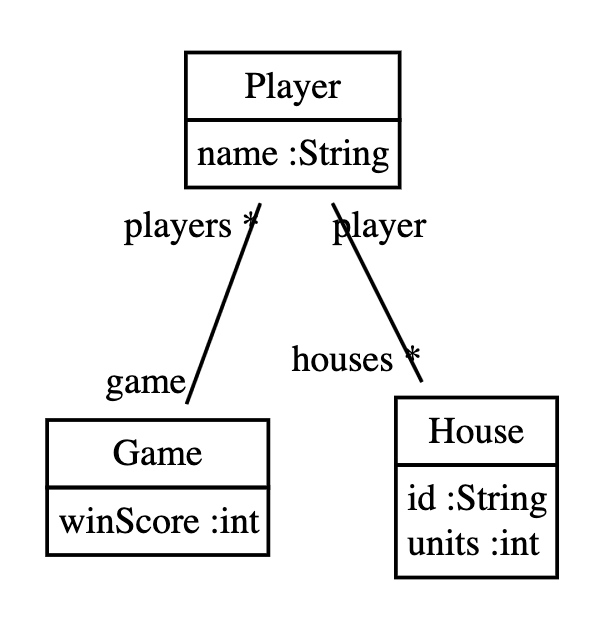
\includegraphics[width=0.4\textwidth]{chapter/pattern-matching/img/game-class-diagram.png}
    \caption{Beispiel-Klassendiagramm zur Verwendung von FulibTables}
    \label{fig:game-class-diagram}
\end{figure}

Es werden nun einige Beispielobjekte zu diesem Modell erstellt, die den Endzustand des Spiels beschreiben.

\begin{jcodeblock*}{breaklines}
    Game game = new Game().setWinScore(60);
    Player alice = new Player().setName("Alice").setGame(game);
    Player bob = new Player().setName("Bob").setGame(game);
    Player charlie = new Player().setName("Charlie").setGame(game);
    House a1 = new House().setId("a1").setUnits(30).setPlayer(alice);
    House a2 = new House().setId("a2").setUnits(20).setPlayer(alice);
    House b1 = new House().setId("b1").setUnits(40).setPlayer(bob);
    House c1 = new House().setId("c1").setUnits(60).setPlayer(charlie);
\end{jcodeblock*}

Das zugehörige Objektdiagramm ist in Abbildung~\ref{fig:game-object-diagram} zu sehen.

\begin{figure}
    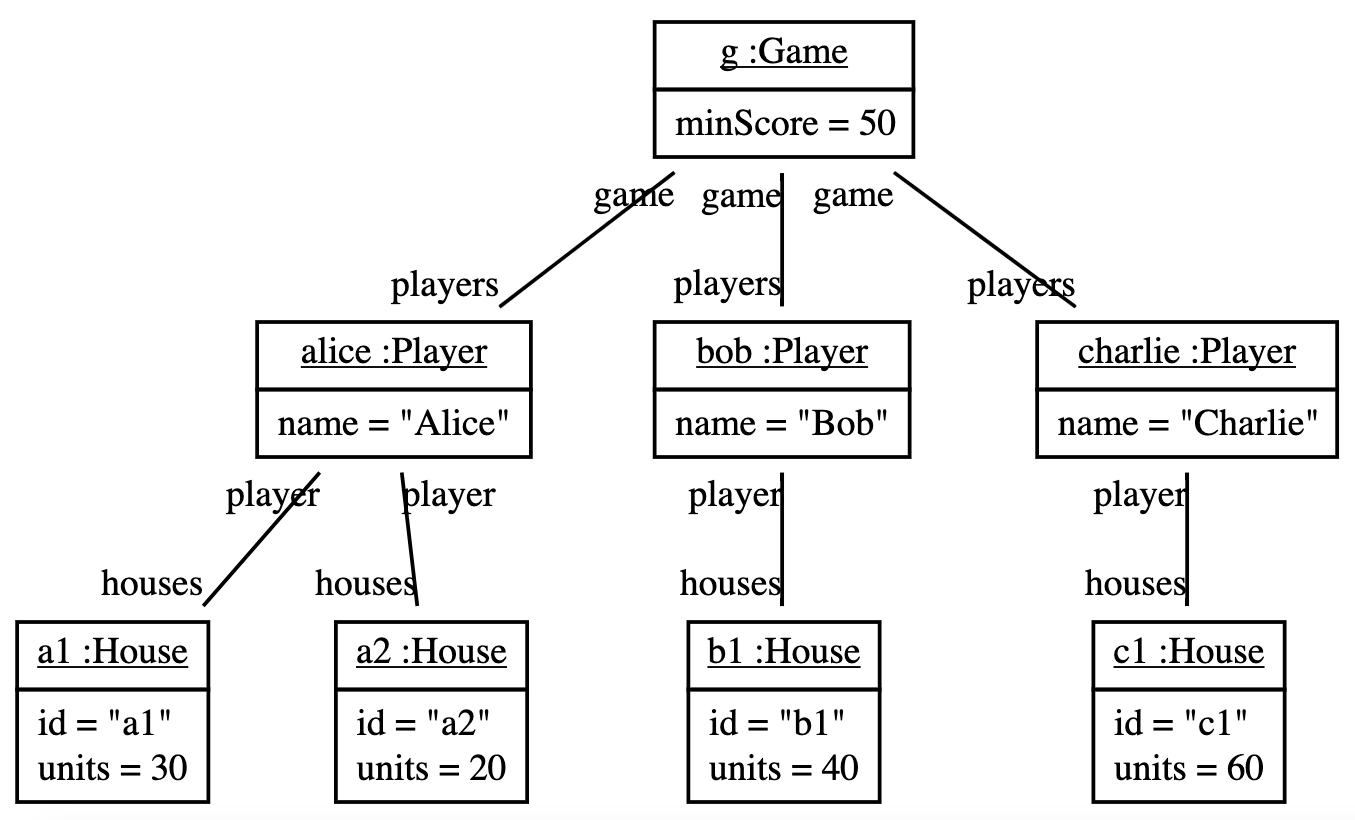
\includegraphics[width=\textwidth]{chapter/pattern-matching/img/game-object-diagram.png}
    \caption{Beispiel-Objektdiagramm zur Verwendung von FulibTables}
    \label{fig:game-object-diagram}
\end{figure}

Nun kann eine Tabelle angelegt werden.
In FulibTables besteht jede Tabelle aus mindestens einer Spalte und null oder mehr Zeilen\footnote{Der Spaltenname zählt dabei nicht als Zeile.}.
Tabellen können \emph{erweitert} oder \emph{eingeschränkt} werden, wobei Spalten entstehen oder entfernt werden.
Beim Erweitern entstehen neue Tabellen-Instanzen,
die sich die Daten der ursprünglichen Tabelle teilen.
Jede Tabellen-Instanz hat eine Spalte, auf die sie \emph{zeigt}.
Operationen auf der Tabelle beziehen sich i.d.R.\ auf diese Spalte,
wirken sich aber durch das geteilte Datenmodell auf alle anderen Instanzen aus.
Zunächst wird nur eine einfache Tabelle mit einer Spalte und einer Zeile benötigt.
Dafür müssen der Name der ersten Spalte sowie eine Liste von Objekten, die die Zeilen dieser Spalte bilden, angegeben werden.
Hier wird zunächst nur eine Zeile gebraucht.

\begin{jcodeblock}
    ObjectTable<Game> games = new ObjectTable<>("Games", game);
\end{jcodeblock}

Diese lässt sich wie folgt darstellen:

\begin{tabular}{|c|}
    \hline
    \textbf{Games} \\
    \hline
    g \\
    \hline
\end{tabular}

Auf dieser Tabelle lässt sich nun eine Erweiterung durchführen, was mit der Methode \code{expand} erreicht wird.
Diese erwartet zuerst einen Namen für die neue Spalte, die sowohl der alten Tabelle hinzugefügt wird als auch Ziel der neuen Tabellen-Instanz ist.
Weiterhin wird eine Funktion in Form eines Lambda-Ausdrucks übergeben.
Dieser wird für jede Zeile der Tabelle aufgerufen.
Die Ergebnisse bilden dann die Zeilen der neuen Spalte.
Dies wird anhand des Beispiels deutlich:

\begin{jcodeblock*}{breaklines,escapeinside=||}
    Table<Integer> winScores = games.expand("Win Scores", Game::getWinScore|\footnotemark|);
\end{jcodeblock*}
\footnotetext{Bei diesem Ausdruck handelt es sich um eine Methodenreferenz, die zu dem Lambda-Ausdruck \jcode{game -> game.getWinScore()} äquivalent ist.}

Die neue Tabelle lässt sich wie folgt darstellen:

\begin{tabular}{|c|c|}
    \hline
    \textbf{Games} & \textbf{Win Scores} \\
    \hline
    g & 60 \\
    \hline
\end{tabular}

Die \code{expand}-Methode ist geeignet für Attribute und Zu-1-Assoziationen.
Für Zu-N-Assoziationen kommt die \code{expandAll}-Methode zum Einsatz.
Diese erwartet ebenfalls einen Spaltennamen und einen Lambda-Ausdruck,
allerdings muss letzterer eine Liste von Werten zurückgegeben.
Für jedes Element dieser Listen wird eine neue Zeile angelegt.

\begin{jcodeblock*}{breaklines}
    ObjectTable<Player> players = games.expandAll("Players", Game::getPlayers);
\end{jcodeblock*}

\begin{tabular}{|c|c|c|}
    \hline
    \textbf{Games} & \textbf{Win Scores} & \textbf{Players} \\
    \hline
    g & 60 & Alice   \\
    g & 60 & Bob     \\
    g & 60 & Charlie \\
    \hline
\end{tabular}

Um das Verhalten zu verdeutlichen, wird eine weitere \code{expandAll}-Operation auf der entstandenen Tabelle durchgeführt.
Da Alice zwei Häuser hat, wird ihre Zeile dupliziert.
Bei Bob und Charlie ist dies nicht der Fall.

\begin{jcodeblock*}{breaklines}
    ObjectTable<House> houses = players.expandAll("Houses", Player::getHouses);
\end{jcodeblock*}

\begin{tabular}{|c|c|c|c|}
    \hline
    \textbf{Games} & \textbf{Win Scores} & \textbf{Players} & \textbf{Houses} \\
    \hline
    g & 60 & Alice   & a1 \\
    g & 60 & Alice   & a2 \\
    g & 60 & Bob     & b1 \\
    g & 60 & Charlie & c1 \\
    \hline
\end{tabular}

U.U.\ ist der Name des zu erweiternden Attributs nicht bekannt.
Dafür wurde als Teil dieser Arbeit eine alternative \code{expandAll}-Operation entwickelt,
bei der dieser nicht angegeben werden muss.
Diese bekommt keinen Lambda-Ausdruck übergeben, sondern ermittelt die existierenden Attribute und Assoziationen der Objekte zur Laufzeit mittels Reflection.

\begin{jcodeblock}
    Table<?> houseAttributes = houses.expandAll("House Attributes");
\end{jcodeblock}

Dabei wird aus jedem Attributwert und jedem Assoziationsziel jedes Objekts der Spalte \code{Houses} eine neue Zeile.
Zu-N-Assoziationen und mehrwertige Attribute (Listen) werden dabei abgeflacht.

\begin{tabular}{|c|c|c|c|c|}
    \hline
    \textbf{Games} & \textbf{Win Scores} & \textbf{Players} & \textbf{Houses} & \textbf{House Attributes} \\
    \hline
    g & 60 & Alice   & a1 & a1      \\
    g & 60 & Alice   & a1 & Alice   \\
    g & 60 & Alice   & a1 & 30      \\
    g & 60 & Alice   & a2 & a2      \\
    g & 60 & Alice   & a2 & Alice   \\
    g & 60 & Alice   & a2 & 20      \\
    g & 60 & Bob     & b1 & b1      \\
    g & 60 & Bob     & b1 & Bob     \\
    g & 60 & Bob     & b1 & 40      \\
    g & 60 & Charlie & c1 & c1      \\
    g & 60 & Charlie & c1 & Charlie \\
    g & 60 & Charlie & c1 & 60      \\
    \hline
\end{tabular}

Die Zeilen einer Spalte können nun nach bestimmten Eigenschaften durchsucht werden.
Diese Operation nennt sich \code{filter} und verwendet ebenfalls einen Lambda-Ausdruck,
der angibt, welche Zeilen entfernt und welche behalten werden sollen.
In diesem Beispiel wird unter allen Attributen von Häusern nach ganzen Zahlen gesucht.

\begin{jcodeblock}
    houseAttributes.filter(it -> it instanceof Integer);
\end{jcodeblock}

Dies ergibt die Anzahl der Credits, ohne dass der Name des Attributs angegeben werden musste:

\begin{tabular}{|c|c|c|c|c|}
    \hline
    \textbf{Games} & \textbf{Win Scores} & \textbf{Players} & \textbf{Houses} & \textbf{House Attributes} \\
    \hline
    g & 60 & Alice   & a1 & 30      \\
    g & 60 & Alice   & a2 & 20      \\
    g & 60 & Bob     & b1 & 40      \\
    g & 60 & Charlie & c1 & 60      \\
    \hline
\end{tabular}

Alternativ kann auch eine Filterung über alle Spalten durchgeführt werden, wofür die \code{filterRows}-Operation eingesetzt wird.
Diese erhält einen Lambda-Ausdruck, der für jede Zeile alle Werte erhält.
Die Werte befinden sich in einer Zuordnung (\code{Map}), die einen Spaltennamen zu dem Wert in der Zeile dieser Spalte zuordnet.
Dessen Ergebnis bestimmt wie beim einfachen Filter, ob die Zeile behalten oder entfernt wird.

\begin{jcodeblock}
    houseAttributes.filterRows((Map<String, Object> row) -> {
        int winScore = (int) row.get("Win Scores");
        int units = (int) row.get("House Attributes");
        return units >= winScore;
    });
\end{jcodeblock}

In diesem Beispiel sorgt das dafür, dass alle Zeilen außer die mit dem Spieler Charlie entfernt werden.

\begin{tabular}{|c|c|c|c|c|}
    \hline
    \textbf{Games} & \textbf{Win Scores} & \textbf{Players} & \textbf{Houses} & \textbf{House Attributes} \\
    \hline
    g & 60 & Charlie & c1 & 60 \\
    \hline
\end{tabular}

Die Suche nach einem Gewinner ist nun abgeschlossen.
Aus der Tabelle lässt sich nun ein Ergebnis erzeugen, indem die Tabellenspalte \code{Players} in eine Liste konvertiert wird.

\begin{jcodeblock}
    System.out.println("the winner is: " + players.toList());
    // Output: the winner is: [Charlie]
\end{jcodeblock}

\subsection{Patterns}\label{subsec:patterns}

Patterns sind ein Mechanismus von FulibTables, der die Suche nach Objekten mit bestimmten Eigenschaften in einer Objektstruktur erlaubt.
Die Bibliothek gibt dafür eine einfache API zum Konstruieren von Patterns vor.
Intern wird das Pattern Matching mit Tables realisiert,
die in ihren Operationen gleichmächtig mit Patterns sind.
Jedoch ist die Verwendung von Patterns übersichtlicher und leichter verständlich.
Des Weiteren lassen sich Pattern als Objekte modellieren,
während Tables nur mit einer Folge von Anweisungen bearbeitet werden.
Dadurch lassen sich Patterns deklarativ gebrauchen, während Tables imperativ verwendet werden.

Ein Pattern besteht aus einer Menge von \emph{Pattern-Objekten} und Constraints auf diesen.
Pattern-Objekte dienen als Platzhalter für Objekte und Werte, nach denen gesucht wird,
während Constraints deren Beziehungen modellieren.

Es soll nun die zuvor mit Tables realisiert Suche nach einem Gewinner mit Patterns realisert werden.
Das Datenmodell und die angelegten Objekte werden hier wiederverwendet.
Zunächst werden einige Pattern-Objekte benötigt, um die verschiedenen Arten von Objekten und Werten abzubilden.
Diese lassen sich mit einem \code{PatternBuilder} anlegen.

\begin{jcodeblock*}{breaklines}
    PatternBuilder builder = FulibTables.patternBuilder();

    PatternObject gamePO = builder.buildPatternObject("Game");
    PatternObject winScorePO = builder.buildPatternObject("WinScore");
    PatternObject playerPO = builder.buildPatternObject("Player");
    PatternObject housePO = builder.buildPatternObject("House");
    PatternObject unitsPO = builder.buildPatternObject("Units");
\end{jcodeblock*}

Pattern-Objekte werden nicht nur für Objekte im Datenmodell (z.B.\ \code{gamePO}, \code{playerPO}, \code{housePO}),
sondern auch für deren Attribute benötigt (\code{winScorePO} und \code{unitsPO}).
Intern entspricht jedes Pattern-Objekt einer Spalte der Tabelle, die am Ende des Match-Vorgangs alle Ergebnisse enthält.

Nun müssen die Pattern-Objekte verbunden werden.
Dies geschieht unter Angabe der Attribut- bzw.\ Assoziationsnamen mit der \code{buildPatternLink}-Methode.

\begin{jcodeblock}
    // Attribute:
    builder.buildPatternLink(gamePO, "winScore", winScorePO);
    // Assoziationen:
    builder.buildPatternLink(gamePO, "game", "players", playerPO);
    builder.buildPatternLink(playerPO, "player", "houses", housePO);
    // Beliebige Verknüpfung:
    builder.buildPatternLink(housePO, "*", unitsPO);
\end{jcodeblock}

Zu beachten ist in der letzten Zeile der Name ``\code{*}''.
Dieser dient als Platzhalter für den unbekannten Attributsnamen.
Er bewirkt, dass \code{unitsPO} alle Attribute von \code{housePO} matcht.
Diese Operation ist in Vorbereitung dieser Arbeit aufbauend auf dem zuvor genutzten \code{expandAll} entstanden.
Wie im vorherigen Beispiel sollen sind nicht alle Attribute von Häusern interessant,
weshalb auch hier auf ganze Zahlen eingeschränkt werden soll.
Dafür kommt ein \emph{Attributs-Constraint} zum Einsatz, das wie folgt angelegt wird:

\begin{jcodeblock*}{breaklines}
    builder.buildAttributeConstraint(unitsPO, it -> it instanceof Integer);
\end{jcodeblock*}

Maßgeblich für die Suche nach dem Gewinner ist die Bedingung, dass die Units-Anzahl größer als die vom Spiel vorgegebene Mindestanzahl ist.
Analog zu \code{filterRows} bei Tables kommt dafür bei Patterns ein \emph{Match-Constraint} zum Einsatz,
das wie folgt deklariert wird:

\begin{jcodeblock}
    builder.buildMatchConstraint(row -> {
        int winScore = (int) row.get("WinScore");
        int units = (int) row.get("Units");
        return units >= winScore;
    }, winScorePO, unitsPO);
\end{jcodeblock}

Der Lambda-Ausdruck entspricht hier jenem, der mit \code{filterRows} gebraucht wurde.
Zu beachten ist jedoch hier die Angabe der verwendenden Pattern-Objekte dahinter.
Ohne diese könnten Match-Constraints bei der Suche immer erst als letzte bearbeitet werden,
was u.U.\ zu sehr großen Zwischenergebnissen führen kann.

Nun sind alle Pattern-Objekte und Constraints angelegt.
Mit \code{builder.getPattern()} lässt sich eine Objekt erhalten, dass all diese kapselt.
Das davon ausgehende Objektdiagramm ist in Abbildung~\ref{fig:pattern-diagram} dargestellt.

\begin{figure}
    % TODO \includegraphics[width=\textwidth]{chapter/pattern-matching/img/pattern-diagram.pdf}
    \caption{Objektdiagramm für das erstellte Pattern}
    \label{fig:pattern-diagram}
\end{figure}

Mit dem Pattern kann nun ein Matching durchgeführt werden.
Dafür wird zunächst ein \code{PatternMatcher} benötigt, der auch direkt aus dem \code{builder} angelegt werden kann.
Dem Matcher werden dann ein oder mehr \emph{Root-Objekte} und \emph{Root-Pattern-Objekte} zugewiesen.
Diese entsprechen den Objekten und Pattern-Objekten, bei denen die Suche begonnen wird.
Ferner werden daraus die Zeilen und Spalten der Tabelle, die intern als Datenstruktur dient.

\begin{jcodeblock}
    PatternMatcher matcher = builder.matcher();
    matcher.withRootPatternObjects(gamePO);
    matcher.withRootObjects(game);
\end{jcodeblock}

Die Methode \code{match()} führt nach Einrichten des Matchers den eigentlichen Match-Vorgang durch.
Daraufhin lassen sich die Ergebnisse anhand der Pattern-Objekte extrahieren:

\begin{jcodeblock}
    matcher.match();

    System.out.println("the winner is: " + matcher.findOne(playerPO));
\end{jcodeblock}

\todo{
Interne Tabellen beim Pattern Matching,
}

\section{Pattern Matching in der Scenario-Sprache}\label{sec:scenario-pattern-matching}

Die Scenario-Sprache bietet syntaktische Unterstützung für Pattern Matching mit FulibTables in Form des \code{Match}-Satzes.
Er erlaubt es, in einer kompakten und ausdrucksstarken Weise Patterns zu bauen und auf Objektstrukturen anzuwenden.
Ergebnis des Satzes sind die gefundenen Objekte, welche im weiteren Verlauf des Scenarios verwendet werden können.
Seine umfangreiche Syntax ist Thema dieses Abschnitts.

Ein Match-Satz ist zu erkennen an dem Schlüsselwort \code{match} bzw.\ \code{matches}, dem ein Subjekt voransteht.
Es folgt eine Liste von Pattern-Objekten, die an den Schlüsselwörten \code{some} und \code{all} zu erkennen sind.
Das folgende Beispiel zeigt den einfachsten möglichen Match-Satz, der nach genau einem beliebigen Objekt sucht und es an den Namen \code{o} bindet.

\begin{mdcodeblock}
    There is a Game.

    We match some object g.
\end{mdcodeblock}

Dieser einfache Satz generiert vergleichsweise langen Java-Code, wie unten zu sehen ist.
Es handelt sich dabei um genau jenen Code, der zur Einrichtung von Patterns und eines Matchers sowie zur Extraktion von Ergebnissen aus letzterem benötigt wird.

\begin{jcodeblock*}{breaklines}
    Object g;
    {
        // Pattern:
        PatternBuilder builder = FulibTables.patternBuilder();
        PatternObject gPO = builder.buildPatternObject("g");
        // Matcher
        PatternMatcher matcher = FulibTables.matcher(builder.getPattern());
        matcher.withRootPatternObjects(gPO);
        matcher.withRootObjects(new ReflectorMap("org.example").discoverObjects(game));
        matcher.match();
        // Results
        g = matcher.findOne(gPO);
    }
\end{jcodeblock*}

Auffällig ist hier die Zeile mit \code{withRootObjects}.
Der Aufruf \code{new ReflectorMap("org.example").discoverObjects(game)} bewirkt hier, dass alle von \code{game} ausgehenden Objekte, deren Typ zum Package \code{org.example} gehört, als Root-Objekte behandelt werden.
I.A.\ werden an \code{discoverObjects} alle sich im Scope befindenden Variablen übergeben.
Dabei können auch Objekte, die nicht direkt zugänglich sind, gefunden werden.
Wichtig ist jedoch, dass nicht direkt nach Objekten gesucht werden kann, die nicht zum Package des Scenarios gehören.
Dies betrifft insbesondere einfache Werte wie Zahlen oder Strings.

\subsection{Typ-Constraints}

Statt \code{object} lässt sich im Match-Satz auch ein Typ angeben, auf den das Pattern-Objekt beschränkt sein soll.

\begin{mdcodeblock}
    We match some Game g.
\end{mdcodeblock}

Dies wirkt sich auf das Pattern-Objekts im Java-Code aus.

\begin{jcodeblock}
    PatternObject gPO = builder.buildPatternObject("g", Game.class);
    // äquivalent zu:
    PatternObject gPO = builder.buildPatternObject("g");
    builder.buildAttributeConstraint(gPO, g -> g instanceof Game);
\end{jcodeblock}

\subsection{Attribut-Constraints mit Gleichheit}

Auf Pattern-Objekte in Match-Sätzen folgt eine Liste von Constraints.
Eine einfache Art davon ist ein Attributwert-Constraint.
Wie das folgende Beispiel zeigt, verwendet dieser eine ähnliche Syntax wie die Zuweisung von Attributen bei der Deklaration von Objekten mit \code{There}.

\begin{mdcodeblock}
    There is a Game with min-score 50.

    We match some object g with min-score 50.
\end{mdcodeblock}

Durch Hinzunahme des Constraints kommt im Java-Code ein weiteres Pattern-Objekt hinzu, was von außen jedoch nicht sichtbar ist.
Es ist mit dem Pattern-Objekt von \code{g} über einen Pattern-Link verbunden und wird durch einen Gleichheits-Constraint eingeschränkt.

\begin{jcodeblock*}{breaklines}
    Object g;
    {
        PatternBuilder builder = FulibTables.patternBuilder();
        PatternObject gPO = builder.buildPatternObject("g");
        PatternObject gMinScorePO = builder.buildPatternObject("gMinScore");
        builder.buildPatternLink(gPO, "minScore", gMinScore);
        builder.buildEqualityConstraint(gMinScorePO, 60);
        // Matcher, Results...
    }
\end{jcodeblock*}

\subsection{Attribut-Constraints mit Vergleichsoperatoren}

Attributwert-Constraint müssen nicht nach exakten Werten prüfen.
Sie können stattdessen auch nach bestimmten Bedingungen wie etwa Zahlenvergleiche oder regulären Ausdrücken eingeschränkt werden.
Die Syntax ändert sich dabei leicht durch Verwendung des Schlüsselworts \code{whose}.

\begin{mdcodeblock}
    There is a Player with name Alice.

    We match some object g whose min-score is greater than 0.
    We match some object p1 whose name matches '[Aa]lice'.
\end{mdcodeblock}

Im Java-Code wird aus dem Gleichheits-Constraint ein allgemeiner Attribut-Constraint mit Lambda-Ausdruck.
Außerdem wird der Typ der Attributs-Pattern-Objekte durch die Verwendung mit den Operatoren eingeschränkt.

\begin{jcodeblock*}{breaklines}
    PatternObject gMinScorePO = builder.buildPatternObject("gMinScore", Number.class);
    PatternObject p1NamePO = builder.buildPatternObject("p1Name", String.class);
    // Links...
    builder.buildAttributeConstraint(gMinScorePO, (Number n) -> n.doubleValue() > 0);
    builder.buildAttributeConstraint(p1NamePO, (String s) -> s.matches("[Aa]lice"));
\end{jcodeblock*}

\subsection{Attribut-Constraints mit unbekannten Attribut-Namen}

Die vorherigen Beispiele setzen voraus, dass der Name des Attributs bekannt ist.
Match-Sätze erlauben jedoch, eine Bedingung an ein beliebig benanntes Attribut zu stellen.
Als Platzhalter dient dafür \code{some attribute};
das Schlüsselwort \code{whose} wird zu \code{where}.

\begin{mdcodeblock}
    There is a Player with username Alice.

    We match some object p1 where some attribute matches '[Aa]lice'.
\end{mdcodeblock}

Im Java-Code verändert sich primär der Link zwischen den beiden Pattern-Objekten,
indem der im vorherigen Abschnitt erklärte Verknüpfungsname \code{*} verwendet wird.

\begin{jcodeblock*}{breaklines}
    PatternObject p1Attr1PO = builder.buildPatternObject("p1Attr1", String.class);
    builder.buildPatternLink(p1PO, "*", gMinScore);
    // AttributeConstraint... (s.o.)
\end{jcodeblock*}

\subsection{Mehrere Root-Objekte und Fehlerfälle}

Pattern-Links kommen auch zum Einsatz, wenn nach Assoziationen zwischen Objekten gesucht wird.
Dafür werden zunächst zwei Pattern-Objekte benötigt.
In einem Match-Satz müssen diese lediglich durch \code{and} oder \code{,} getrennt werden:

\begin{mdcodeblock}
    We match some object g and some object p1.
\end{mdcodeblock}

% Unordered List syntax
Eine alternative Schreibweise verwendet jedoch eine Auflisting der Pattern-Objekte mit der Markdown-eigenen Syntax für ungeordnete Listen.
Diese ist aufgrund der Leserlichkeit der einzeiligen Schreibweise vorzuziehen.

\begin{mdcodeblock}
    We match:
    - some object g
    - some object p1.
\end{mdcodeblock}

% Mehrere Root-POs
Beide Schreibweise bewirken, dass sowohl nach \code{g} als auch nach \code{p1} unter allen Root-Objekten gesucht werden kann.

\begin{jcodeblock}
    matcher.withRootPatternObjects(gPO, p1PO);
\end{jcodeblock}

% Ungleichheits-Bedingung
Ferner impliziert die Existenz mehrere Pattern-Objekten im gleichen Match-Satz,
dass diese ungleich sein müssen.
Genau diese Ungleichheits-Bedingung bewirkt,
dass die reine Deklaration mehrerer Pattern-Objekte \emph{nicht} gleichbedeutend mit der Verwendung mehrerer Match-Sätze ist.

\begin{jcodeblock}
    builder.buildDistinctConstraint(gPO, p1PO);
\end{jcodeblock}

% Exceptions
Konkret hat dies die Konsequenz, dass \code{g} und \code{p1} in keinem Fall das selbe Objekt matchen können.
Ohne weitere Einschränkung ist dieses Beispiel also unerfüllbar:
Wird vor dem Match-Satz nur genau ein Objekt deklariert, kann dieses zwar \code{g} zugewiesen werden, jedoch bleibt dann \code{p1} unzugewiesen.
Dies bewirkt ein Fehlschlagen des Match-Vorgangs mit einer \code{NoMatchException}.
Wenn mehr als ein Objekt wie z.B.\ \code{game} und \code{player1} deklariert wurden,
sind sowohl \code{g=game, p1=player1} als auch \code{g=player1, p1=game} mögliche Zuweisungen des Patterns.
Diese Uneindeutigkeit bewirkt, dass der Match-Vorgang mit einer \code{AmbiguousMatchException} abbricht.
Durch Wiedereinführen des Attribut-Constraints des Namens des Spielers kann das Problem behoben werden.
Damit wird die eindeutige Zuweisung \code{g=game, p1=player1} erzwungen.

\subsection{Link-Constraints}

% Some Link To
Es soll nun nach einer Verknüpfung zwischen den andernfalls unabhängigen Objekten gesucht werden.
Ist der Name der Assoziation unwichtig, kommt das Constraint \code{with some link to} zum Einsatz:

\begin{mdcodeblock}
    We match:
    - some object g with some link to p1
    - some object p1 where some attribute matches '[Aa]lice'.
\end{mdcodeblock}

% Beliebige Reihenfolge
Hier ist besonders zu beachten, dass ein Pattern-Objekt vor dessen Deklaration referenziert werden kann.
Dies ist mitunter durch die deklarative Natur des generierten Java-Codes möglich,
in dem zuerst alle Pattern-Objekte und dann deren Constraints erstellt werden.
Der untenstehende Ausschnitt zeigt weiterhin die Zeilen, die die zuvor erwähnte Ungleichheit definiert.

\begin{jcodeblock}
    PatternObject gPO = builder.buildPatternObject("g");
    PatternObject p1PO = builder.buildPatternObject("p1");
    builder.buildPatternLink(gPO, "*", p1PO); // some link to
    // AttributeConstraint...
    builder.buildDistinctConstraint(gPO, p1PO); // Ungleichheit: g != p1
\end{jcodeblock}

% Reversing the link
Würde man stattdessen \code{object p1 ... with some link to g} schreiben,
würde sich dies auf die Semantik auswirken.
Unter \code{some link} ist nämlich eine unidirektionale Assoziation zu verstehen.
Wäre beispielsweise eine solche für die Spieler-Liste des Spiels verwendet wurden,
könnte nur \code{g with some link to p1} diese Verbindung erkennen,
während \code{p1 with some link to g} keine Ergebnisse liefern würde.

\subsection{Benannte Link-Constraints mit Attribut-Constraints}

% Named Links with Attribute Constraints
Bei Link-Constraints kann auch der Name der Assoziation angegeben werden.
Dies ist möglich, indem man die gleiche Syntax wie für Attribute verwendet,
aber als Attributwert den Namen eines Pattern-Objekts angibt:

\begin{mdcodeblock}
    We match:
    - some object g with players p1
    - some object p1 where some attribute matches '[Aa]lice'.
\end{mdcodeblock}

Der Java-Code errinnert stark an jenen, der zuvor für das reguläre Attribut-Constraint generiert wurde:

\begin{jcodeblock}
    final PatternObject gPO = builder.buildPatternObject("g");
    final PatternObject p1PO = builder.buildPatternObject("p1");
    builder.buildPatternLink(gPO, "players", p1PO);
\end{jcodeblock}

% Attributes as POs
Der wesentliche Unterschied ist, dass zuvor das Attribut-Pattern-Objekt \code{gMinScore} nur der Einschränkung diente und nach dem Match-Vorgang verworfen wurde,
\code{p1PO} jedoch auch an die Variable \code{p1} gebunden wird und somit später verfügbar ist.
Diese Eigenschaft lässt sich auch für Attribute nutzen, deren Wert später zugänglich gemacht werden soll.
So kann durch Hinzufügen eines explizit benannten Root-Pattern-Objekts der Wert von \code{minScore} ermittelt werden:

\begin{mdcodeblock}
    We match:
    - some object g with min-score ms
    - some integer ms
    We expect that ms is 50.
\end{mdcodeblock}

Statt \code{with min-score} kann auch \code{where some attribute is} eingesetzt werden, wenn der Name des Attributs nicht bekannt ist.
Sogar \code{with some link to} wäre hier einsetzbar und semantisch äquivalent,
davon ist jedoch abzuraten, da es sich bei \code{ws} um einen Wert und kein Objekt im Sinne der Modellierung handelt.

\subsection{Match-Constraints}

Auch Match-Constraints werden von der Scenario-Sprache in Match-Sätzen unterstützt.
Dafür kommt erneut das Schlüsselwort \code{where} zum Einsatz.
Auf dieses folgt eine beliebiger Bedingungsausdruck, die beliebig viele andere Pattern-Objekte des gleichen Match-Satzes enthalten kann.

\begin{mdcodeblock*}{breaklines}
    We match:
    - some game g
    - some player p1
    where min-score of g is 0 or score of p1 is greater than min-score of g.
\end{mdcodeblock*}

Obwohl das Match-Constraint zum vorstehenden Pattern-Objekt gehört, bietet es sich zur Übersichtlichkeit an,
diesen hinter unter Liste von Pattern-Objekten zu platzieren.
Im Java-Code ist ersichtlich, dass automatisch die Abhängigkeit des Constraints auf die Pattern-Objekte \code{g} und \code{p1} erkannt wurde.
Des Weiteren wurden deren Namen im Bedingungsausdruck durch Hilfsvariablen ersetzt, da die eigentlichen Variablen noch nicht verfügbar sind.

\begin{jcodeblock*}{breaklines}
    builder.buildMatchConstraint(row -> {
        Game _g = (Game) row.get("g");
        Player _p1 = (Player) row.get("p1");
        return _g.getMinScore() == 0 || _p1.getScore() > _g.getMinScore();
    }, gPO, p1PO);
\end{jcodeblock*}

\todo{find all}

\section{Pattern Matching in Assignments}\label{sec:assignment-pattern-matching}

	\chapter{Ergebnisse}\label{ch:ergebnisse}

Unter Berufung auf die in Kapitel~\ref{ch:goals} gesteckten Ziele soll nun eine Einschätzung erfolgen, inwiefern diese erreicht wurden.
Außerdem gilt es zu betrachten, welche Schwierigkeiten bei der Umsetzung überwunden und welche Erkenntnisse damit gewonnen wurden.

Das FulibScenarios-Projekt stellte aufgrund des großen Umfangs eine Herausforderung dar.
Dies begann mit dem Design der Sprache, das gezielte Anpassung an den vorgesehenen Einsatz im Story Driven Modeling erforderte.
Der Einsatz natürlicher Sprache setzte neue Ideen hinsichtlich der Syntax voraus, da nicht auf in anderen Programmiersprachen übliche Konstrukte wie geschweifte Klammern oder Einrückung zurückgegriffen werden konnte.
Dies ermöglichte jedoch die leichte Verständlichkeit beim Lesen auch für Personen mit nicht-technischem Hintergrund.
Das Schreiben setzt durch die syntaktischen Anforderungen einen Entwickler voraus, ohne diese wäre jedoch die eindeutige Semantik und somit die Ableitung von Diagrammen und Tests nicht möglich.
Auch die Integration in Markdown, die letztlich die Verwendung als Dokumentation erlaubt, musste in der Designphase beachtet werden.
Da dieses Format vielen Entwicklern durch Platformen wie GitHub bekannt ist, erlaubt es den schnellen Einstieg in die Grundlagen der Scenario-Sprache.

Die Entwicklung des Compilers setzte eine bedachte Architektur voraus, um die Vielzahl von Funktionalität übersichtlich und wartbar zu machen.
Der Gebrauch von FulibScenarios wurde von Studierenden zwar nur mittelmäßig bewertet,
dies lag aber zu großen Teilen an der mangelnden Dokumentation und anderen Problemen, die inzwischen behoben wurden.
Das FulibScenarios-Projekt ist jedoch noch nicht vollendet;
weitere Änderungen und neue Features sind bereits geplant.

Die Implementierung der Mustererkennung wurde sehr durch die bestehende FulibTables-Bibliothek unterstützt.
Auch die Erweiterung, die das Abstrahieren über Namen erlaubte, konnte mit relativ geringem Aufwand durchgeführt werden.
Einzig die Einbettung in die Scenario-Sprache stellte eine besondere Herausforderung dar.
Die Konzepte von FulibTables mussten dafür in ein umgängliches, natürliches Sprachformat verpackt werden.
Wie das Beispiel im vorherigen Kapitel gezeigt hat, ist es dennoch gelungen, eine verständliche Syntax zu definieren und zu implementieren.
Auch hier ist es angebracht, neue Einsatzmöglichkeiten zu erproben und die Funktionalität zu erweitern.
Da es sich um neue Sprachkonzepte handelt, konnten diese insbesondere noch nicht in einem praktischen Kontext wie etwa mit Studierenden angewendet werden.

Die Hauptseite von fulib.org hat sich seit ihrer Erstellung als nützliches Werkzeug bewährt.
Auch beim Verfassen dieser Arbeit wurde sie vermehrt eingesetzt, um Beispiele der Scenario-Sprache zu erstellen und zu prüfen.
Ohne die Seite wäre das mühsame Einrichten eines Projekts von Nöten gewesen.
Der einfache Einstieg war letztlich auch in der Vorlesung Programmieren und Modellieren von Vorteil.
Durch die Beispielszenarien und das sofortige Feedback konnten die Studierenden schnell die notwendigen Aspekte der Scenario-Sprache erlernen.
Besonders die Aufzeichnung von Anfragen ermöglichte es, Probleme in Sprache und Compiler zu erkennen und häufige Fehlerfälle mit besseren Hinweisen auszustatten.
Die Umfrage zeigte, welche Features in Zukunft priorisiert hinzugefügt werden müssen.

Bei der Entwicklung der Assignment-Funktionalität auf fulib.org konnten viele Erkenntnisse in der Frontendentwicklung gewonnen werden.
Ursprünglich nur mit JavaScript, HTML und CSS geschrieben, wurde schnell deutlich, dass diese nicht für die steigenden Anforderungen und damit verbundene Komplexität geeignet sind.
Der Umstieg auf das Angular-Framework konnte diese Einschränkung umgehen und gleichzeitig viele weitere Probleme beheben, die zuvor bestanden.
Die gesteckten Ziele bzgl.\ Aufgabenblättern konnten alle umgesetzt werden.
Letztlich wurde sogar das ursprünglich nicht geplante Feature der Kurse hinzugefügt, die besonders bei unbaufsichtigen Lehrangeboten von Wert sind.
Aber auch fulib.org ist als Projekt noch nicht abgeschlossen.
Ein wichtiger Aspekt, der nicht im Rahmen dieser Arbeit lag, ist die Implementierung eines vollwertigen Benutzersystems.
Der Einsatz der Tokens zur Zugriffskontrolle soll damit ersetzt werden.
Mit einem Benutzersystem verbunden sind Bedenken zu Sicherheit und Datenschutz, die Aufgrund des Umfangs nicht näher betrachtet werden konnten.
Auch der Einsatz in einer größeren Testgruppe von Studierenden ist in Zukunft angebracht, um weitere Verbesserungsmöglichkeiten zu finden und zu realisieren.


	\bibliographystyle{alphadin}
	\bibliography{thesis}

	\listoffigures
	\listoftables
	\renewcommand{\listoflistingscaption}{Listing-Verzeichnis}
	\listoflistings

	\appendix
	\chapter{Anhang}\label{ch:appendix}

\section{Vollständiger Java-Code für UserRegistry-Beispiel}\label{sec:user-registry-full}

\begin{center}
    \code{User.java}
    \inputminted[breaklines]{java}{chapter/fulib-scenarios/java/User.java}

    \code{UserRegistry.java}
    \inputminted[breaklines]{java}{chapter/fulib-scenarios/java/UserRegistry.java}

    \code{UserRegistryTest.java}
    \inputminted[breaklines]{java}{chapter/fulib-scenarios/java/UserRegistryTest.java}
\end{center}

\section{Scenario-Lexer-Grammatik}\label{sec:scenario-lexer-grammar}

\inputminted[breaklines]{antlr}{chapter/fulib-scenarios/grammars/ScenarioLexer.g4}

\section{Scenario-Parser-Grammatik}\label{sec:scenario-parser-grammar}

\inputminted[breaklines]{antlr}{chapter/fulib-scenarios/grammars/ScenarioParser.g4}

\section{GenTreeSrc-Definitionsdatei}\label{sec:gts-definitions}

\inputminted[breaklines]{java}{chapter/fulib-scenarios/definitions/FulibScenarios.gts}

\section{Ergebnisse der Vorlesungsumfrage PM 19/20 zu fulib.org, FulibScenarios und FulibMockups}\label{sec:survey-results}

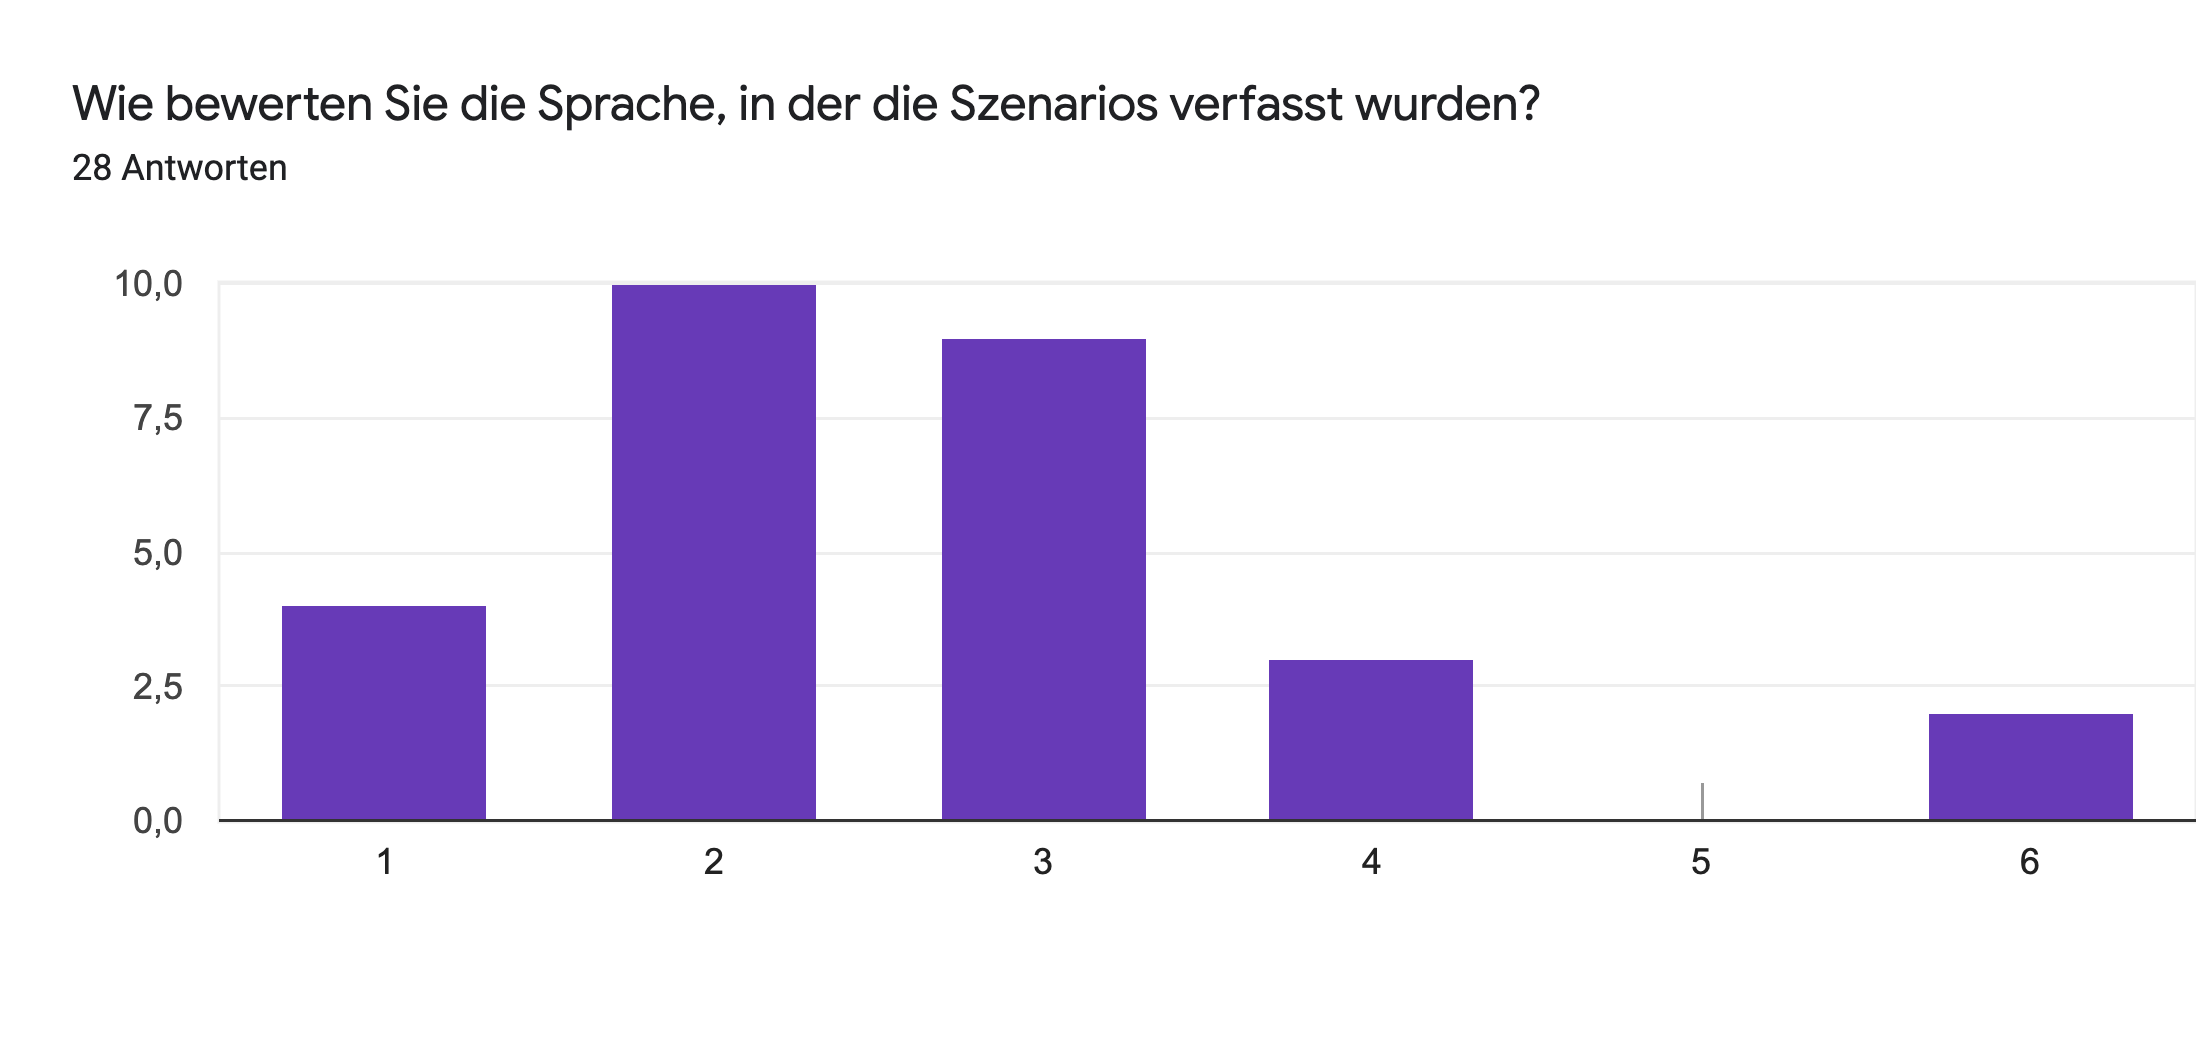
\includegraphics[width=\textwidth]{images/language.png}
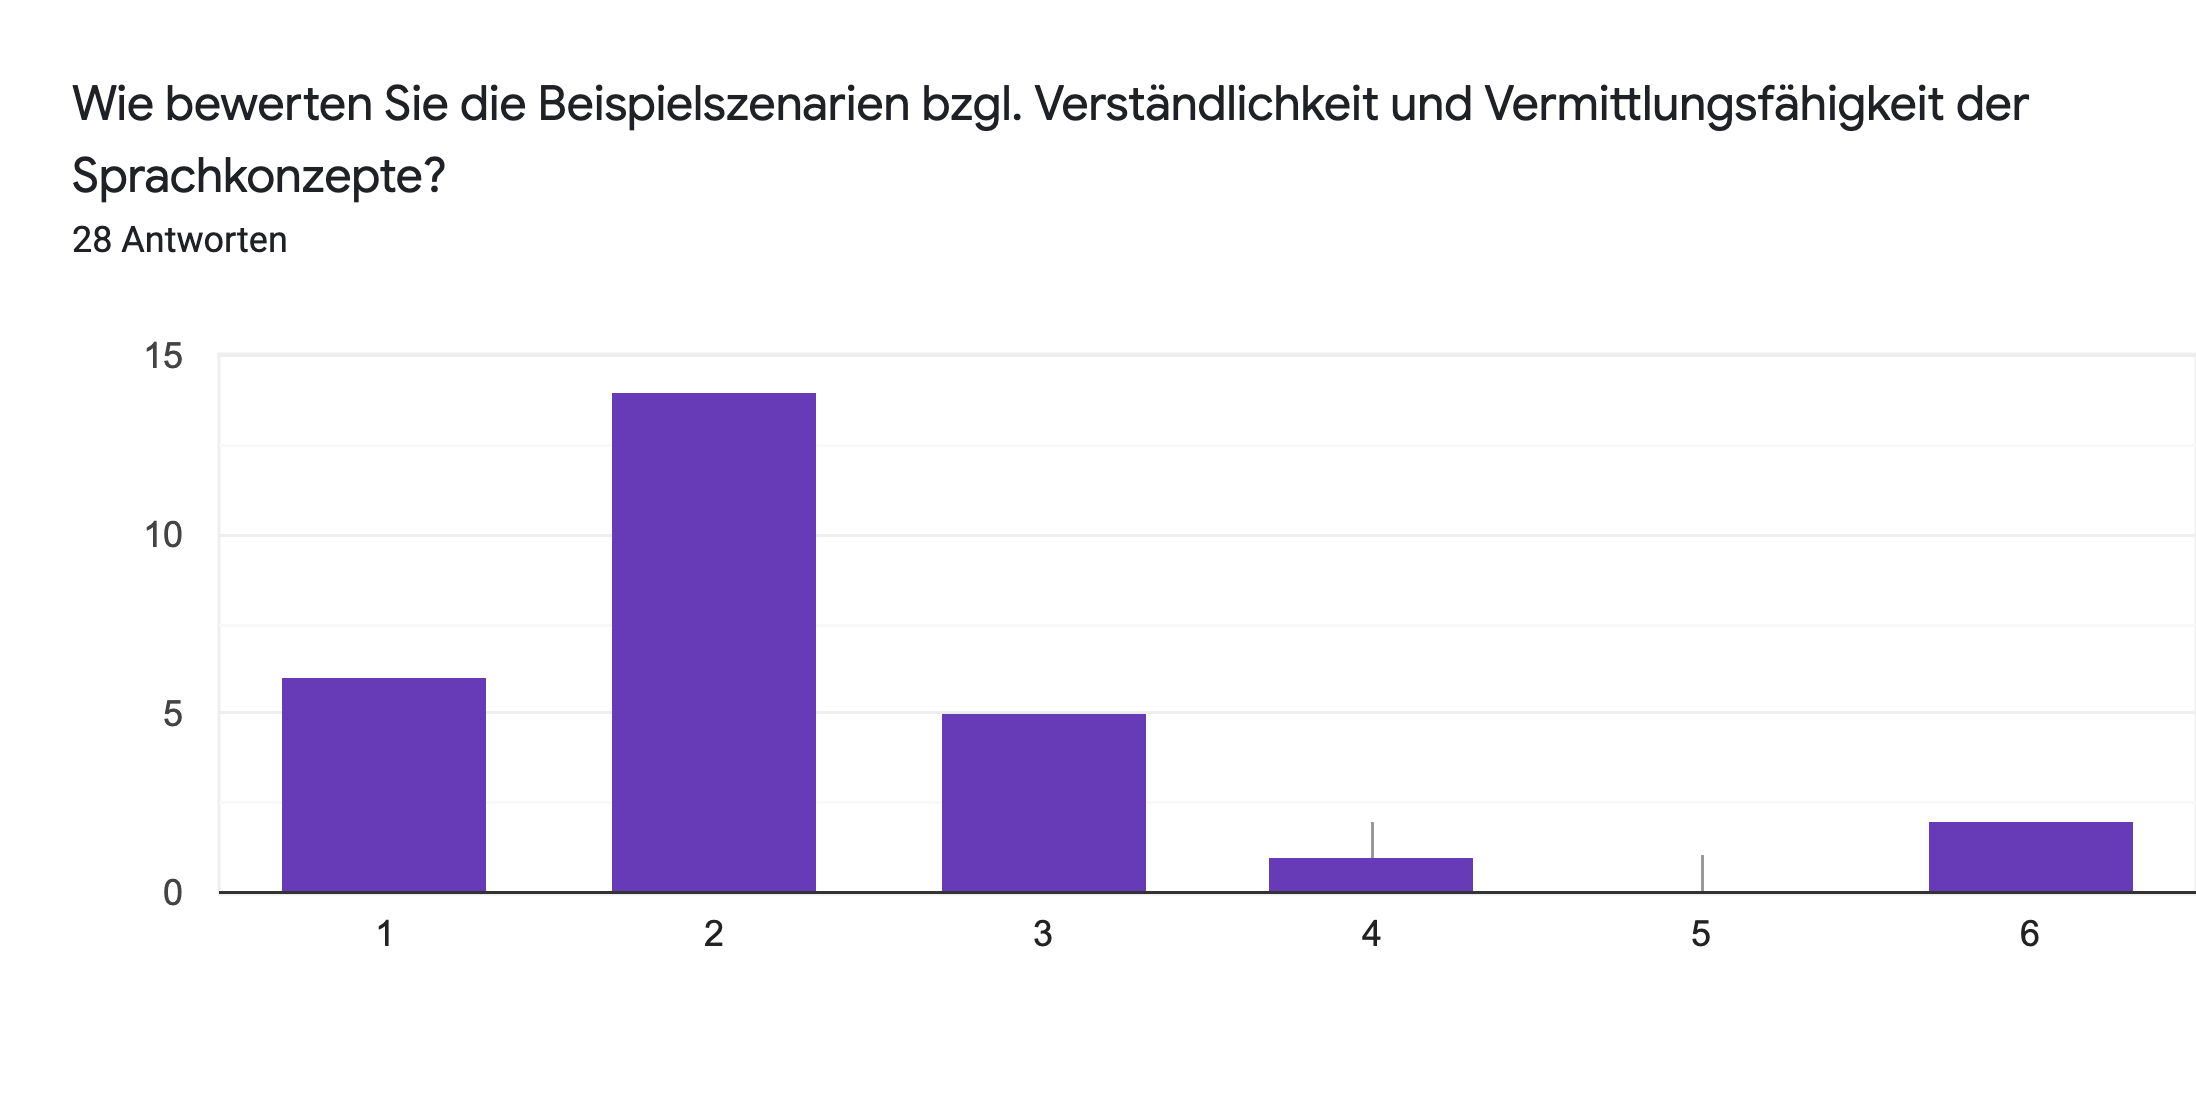
\includegraphics[width=\textwidth]{images/examples.png}
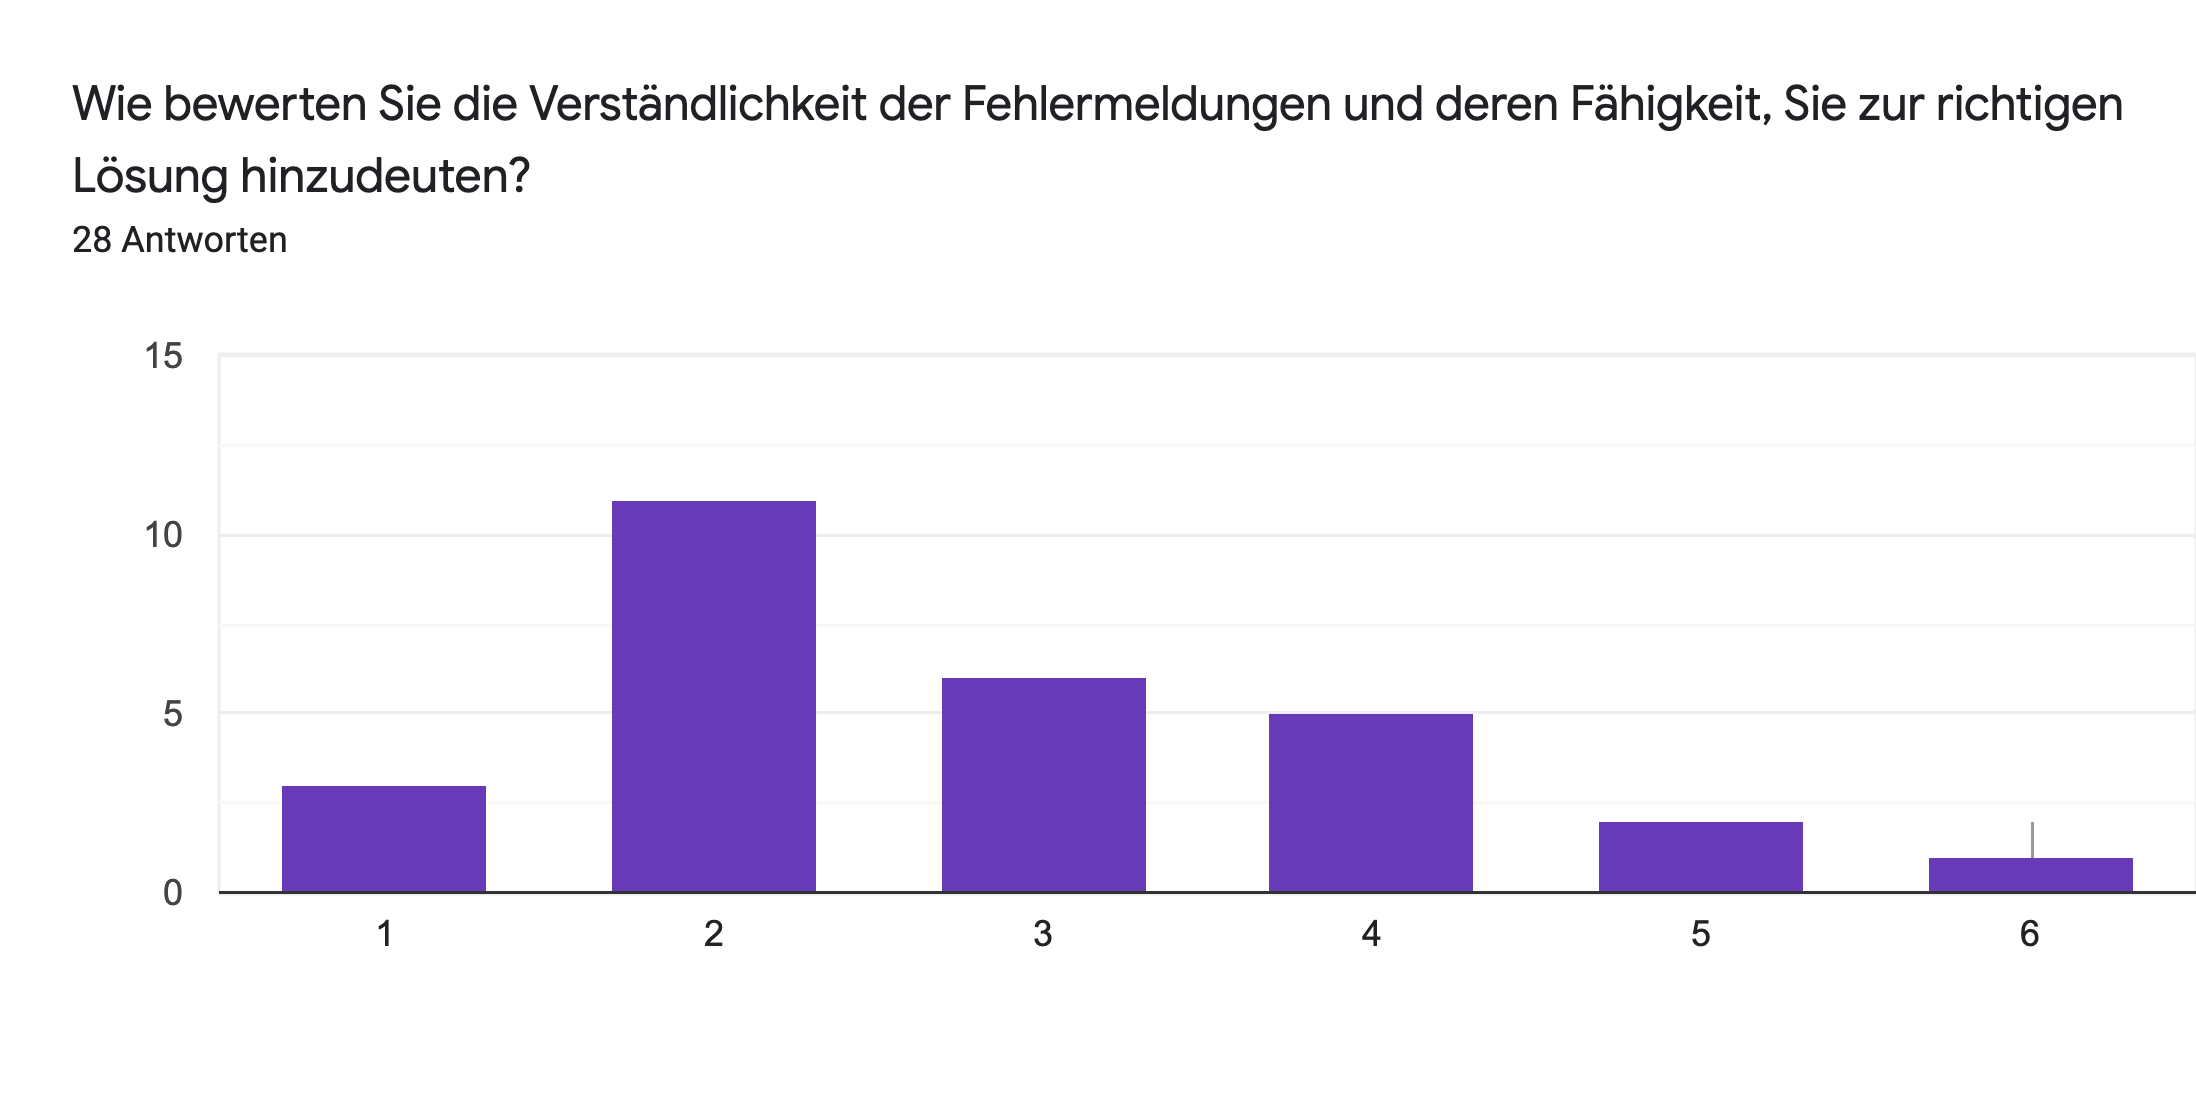
\includegraphics[width=\textwidth]{images/errors.png}
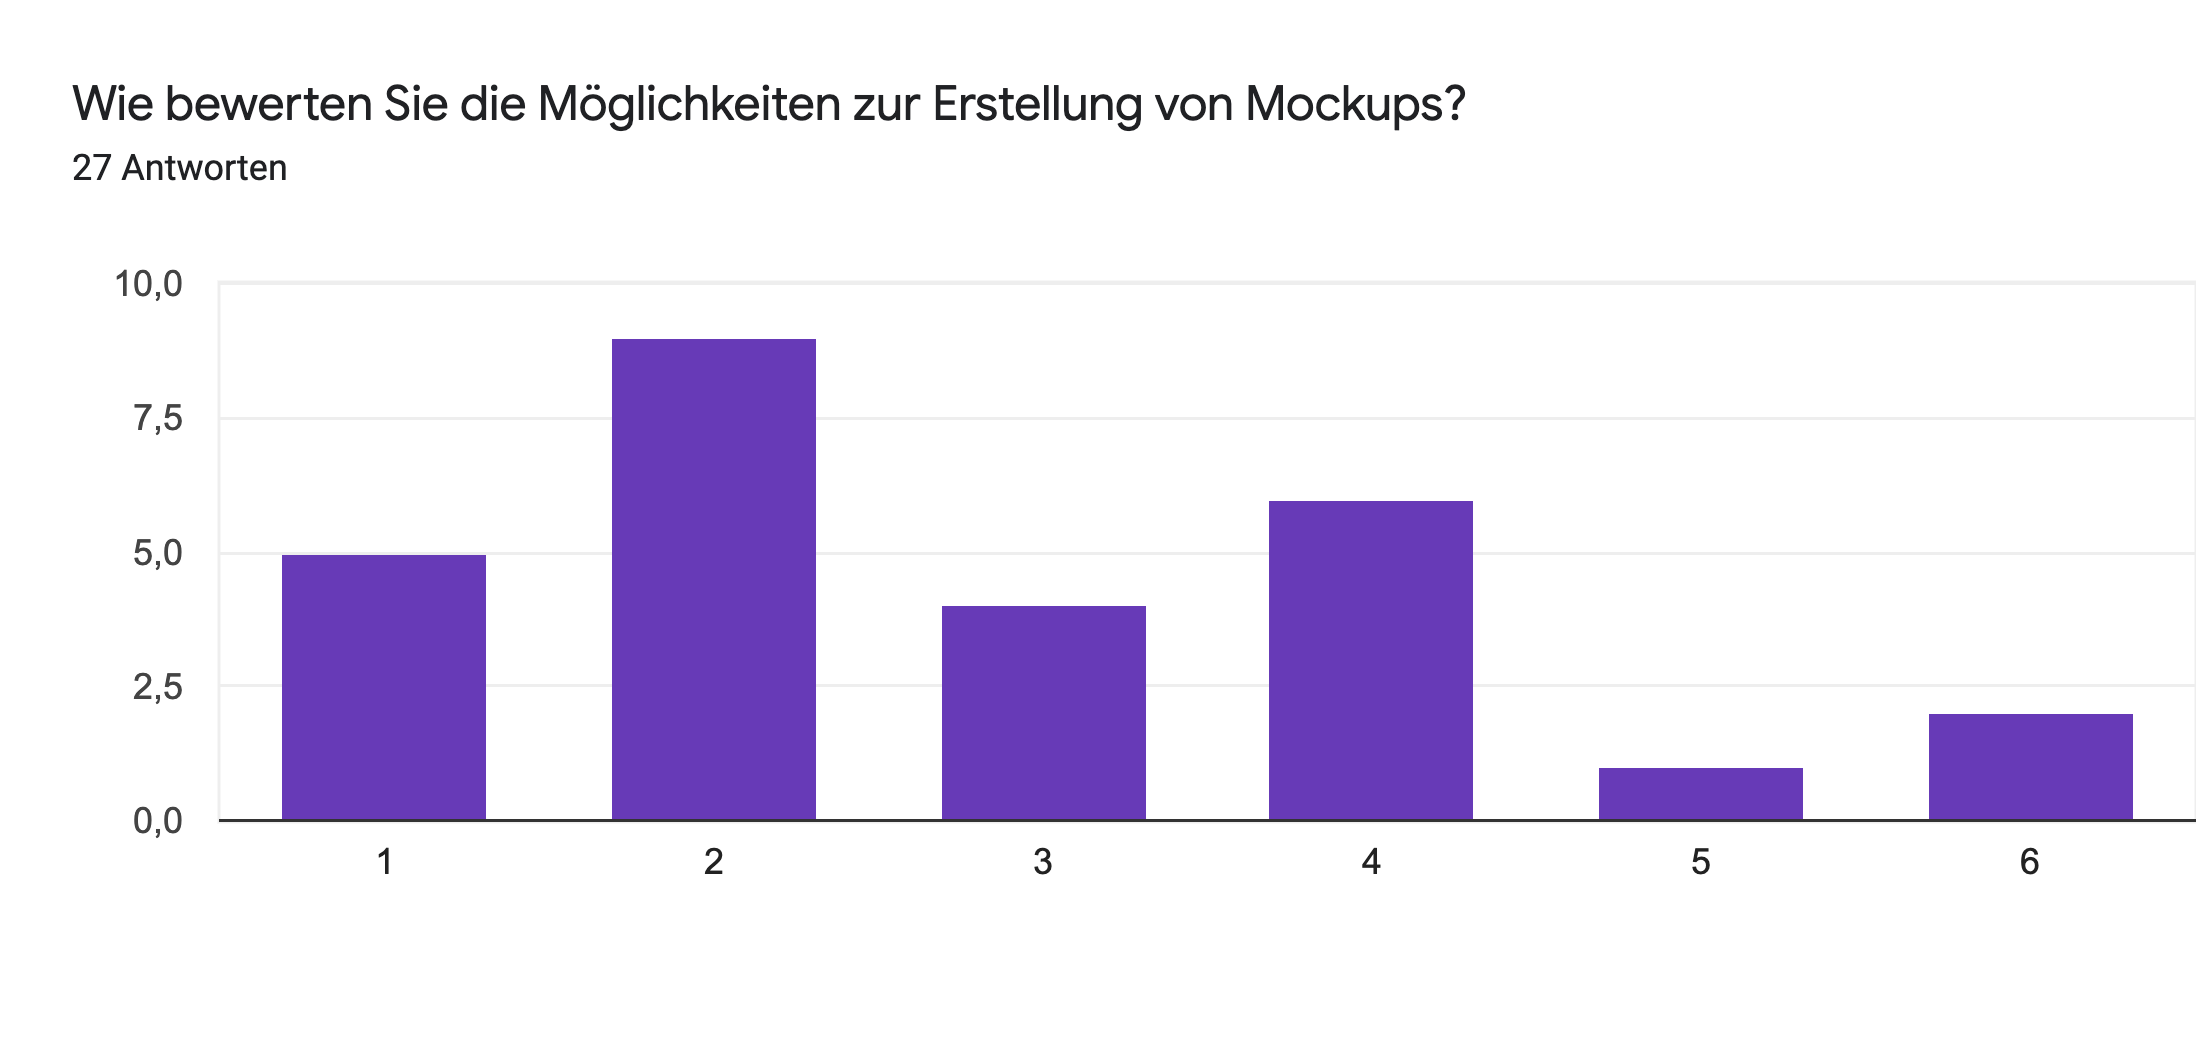
\includegraphics[width=\textwidth]{images/mockups.png}
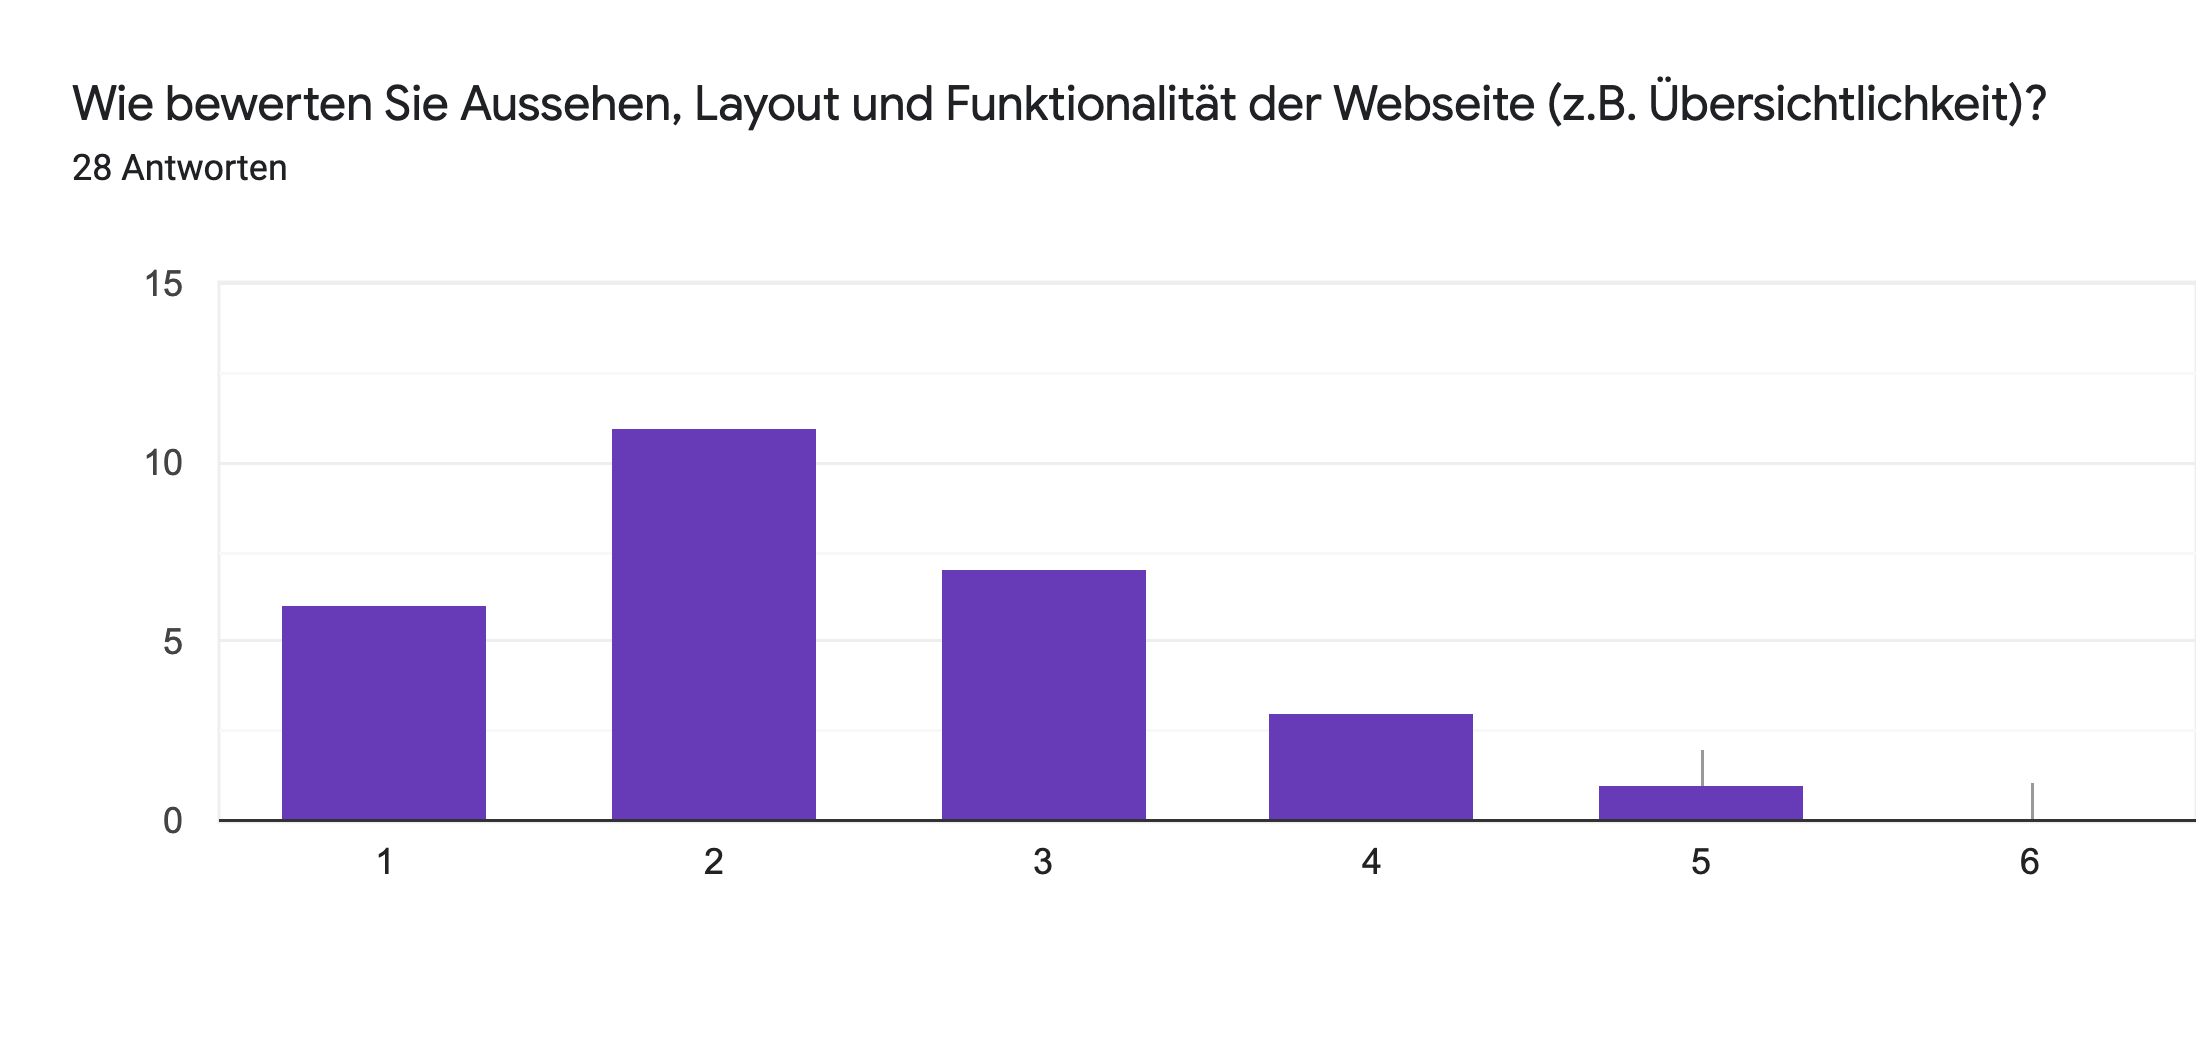
\includegraphics[width=\textwidth]{images/website.png}
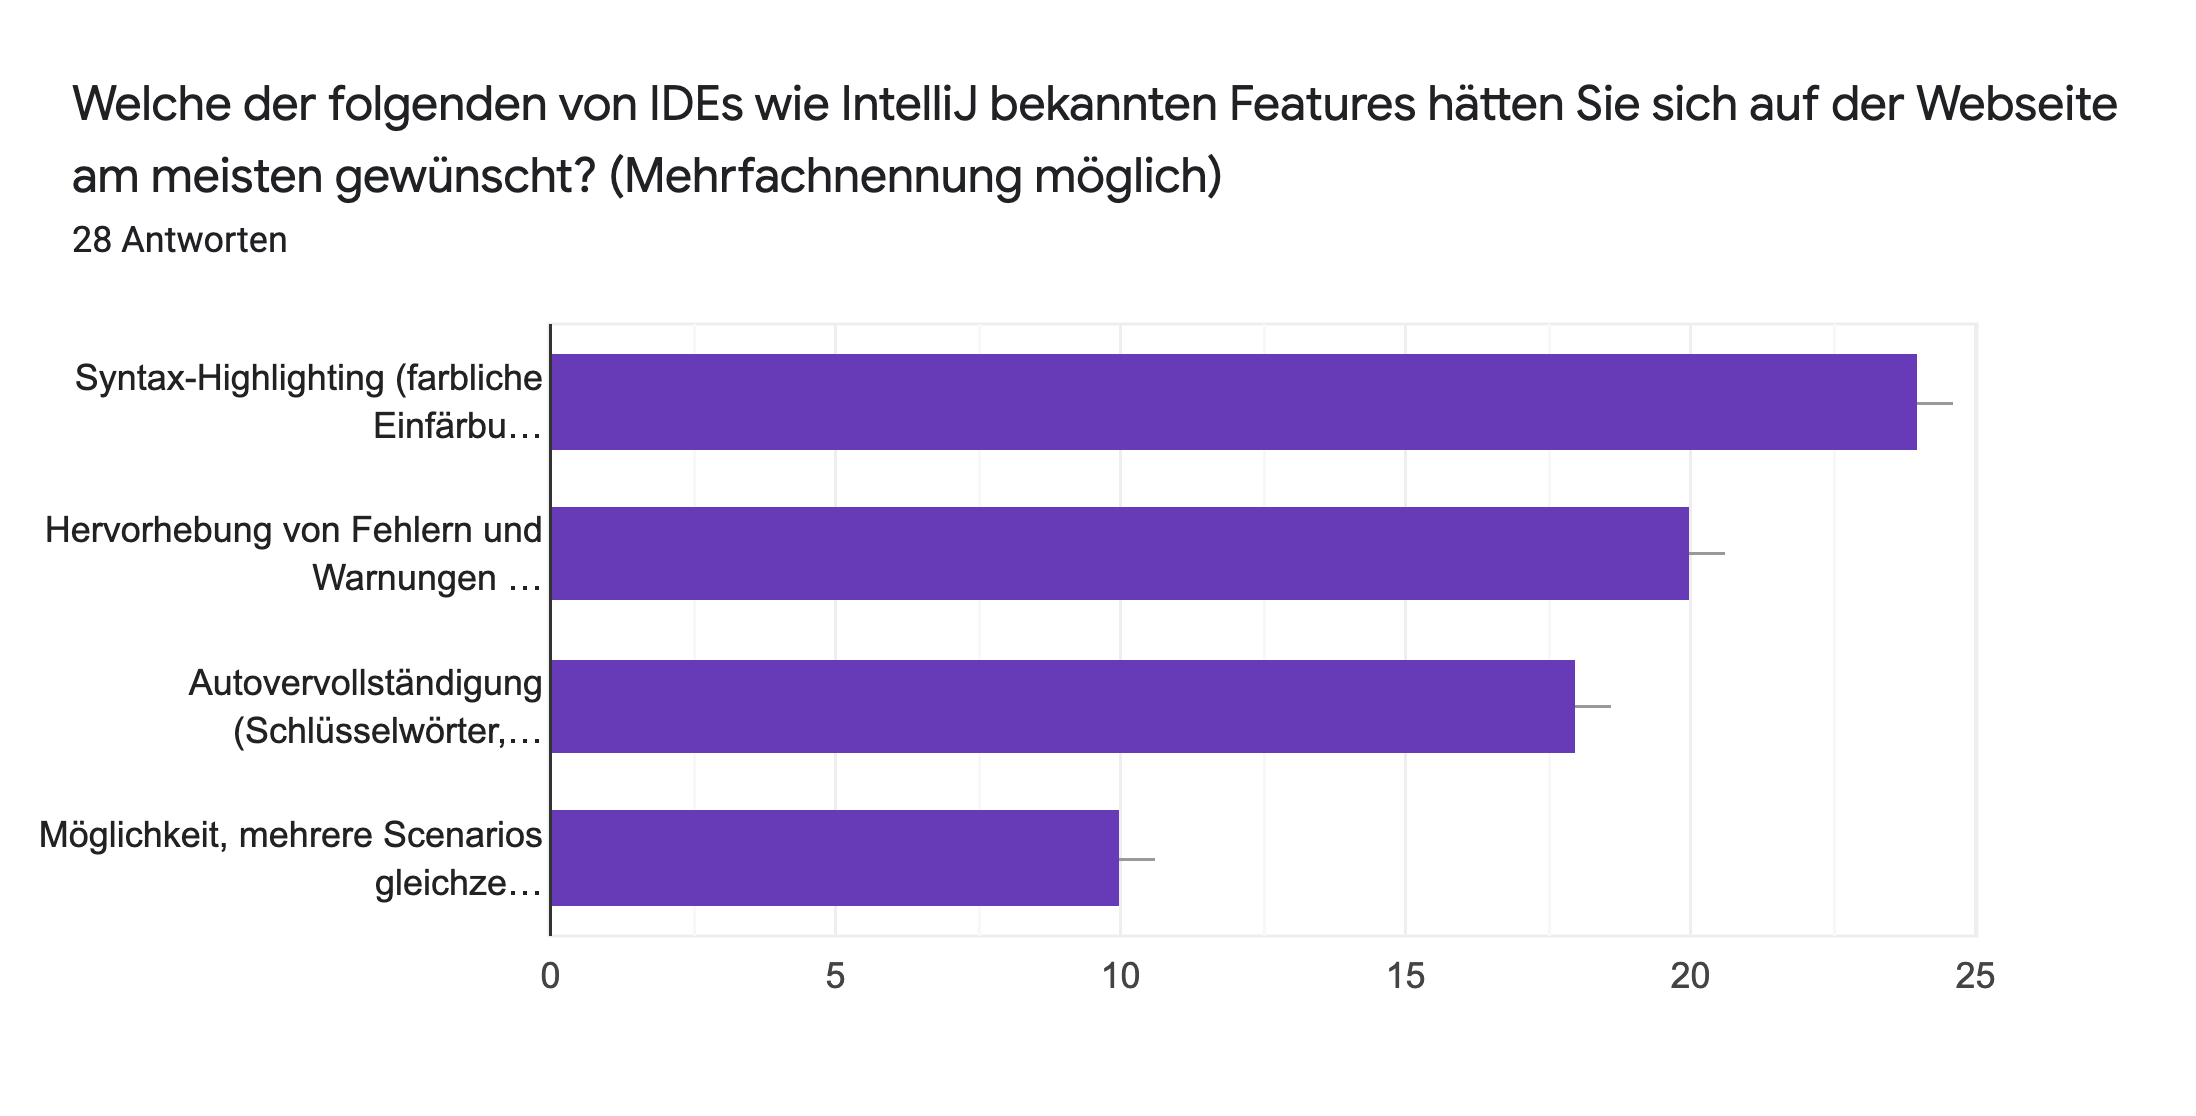
\includegraphics[width=\textwidth]{images/editor-features.png}

%Some guidelines and examples are given in the following.
%
%\section{Figures}
%
%A simple example of a figure can be found in \fig{fig:simple_figure}. A more complex figure including subfigures is show in \fig{fig:figure_with_subfigures}. Here each subfigure can be addressed separately (e.g., \fig{fig:subfigure1} and \fig{fig:subfigure2}). Please use vector graphics (pdf, eps obtained from svg, etc.) whenever possible. Pixel formats like jpeg, bmp, etc. should only be used for real photographs.
%
%\begin{figure}[!h]
%	\centering
%	\fbox{\parbox{5cm}{\centering ~\vspace{1.5cm}\\Dummy\\~\vspace{1.5cm}}} %replace this line by: \includegraphics{path to image}
%	\caption{Simple figure}
%	\label{fig:simple_figure}
%\end{figure}
%
%\begin{figure}[!h]
%	\centering
%	\begin{subfigure}[b]{7cm}
%		\centering
%		\fbox{\parbox{5cm}{\centering ~\vspace{1.5cm}\\Dummy\\~\vspace{1.5cm}}} %replace this line by: \includegraphics{path to image}
%		\caption{Caption of subfigure a (can be empty)}
%		\label{fig:subfigure1}
%	\end{subfigure}
%	\begin{subfigure}[b]{7cm}
%		\centering
%		\fbox{\parbox{5cm}{\centering ~\vspace{1.5cm}\\Dummy\\~\vspace{1.5cm}}} %replace this line by: \includegraphics{path to image}
%		\caption{Caption of subfigure b (can be empty)}
%		\label{fig:subfigure2}
%	\end{subfigure}
%	\caption{Figure using subfigures}
%	\label{fig:figure_with_subfigures}
%\end{figure}
%
%
%\section{Tables}
%
%Examples of tables can be found in \tab{tab:simple_table} and \tab{tab:complex_table}. In general vertical lines are not necessary and should be avoided (see \cite{Fear05} for more about table styles).
%
%\begin{table}[!h]
%	\renewcommand{\arraystretch}{1.1}
%	\caption{A very simple table}
%	\label{tab:simple_table}
%	\centering
%	\begin{tabular}{cccc}
%		\toprule
%		& Apple & Orange & Banana \\
%		\midrule
%		Colour       & green & orange & yellow\\
%		\bottomrule
%	\end{tabular}
%\end{table}
%
%\begin{table}[!h]
%	\renewcommand{\arraystretch}{1.1}
%	\caption{An example of a more complex table}
%	\label{tab:complex_table}
%	\centering
%	\begin{tabular}{ccC{1cm}C{1cm}C{1cm}C{1cm}C{1cm}C{1cm}C{1cm}C{1cm}C{1cm}C{1cm}C{1cm}}
%		\toprule
%		& & \multicolumn{4}{c}{RPAG algorithm} & \multicolumn{5}{c}{RPAGT (proposed)}\\
%		\cmidrule(rl){3-6} \cmidrule(rl){7-11}
%		$N$ & $N_\text{uq}$ & S & add ops & pure reg. & reg. ops & S & add ops & pure reg. & reg. ops & impr.\\
%		\cmidrule(rl){1-11}
%		6   & 3  & 3 & 8  & 1 & 9  & 2 & 5  & 0 & 5  & 44.4\% \\
%		10  & 5  & 3 & 10 & 3 & 13 & 2 & 6  & 2 & 8  & 38.5\% \\
%		13  & 7  & 3 & 14 & 2 & 16 & 2 & 8  & 2 & 10 & 37.5\% \\
%		20  & 10 & 3 & 15 & 4 & 18 & 2 & 9  & 3 & 12 & 33.3\% \\
%		28  & 14 & 3 & 20 & 3 & 23 & 2 & 15 & 2 & 17 & 26.1\% \\
%		41  & 21 & 3 & 31 & 1 & 32 & 2 & 23 & 2 & 25 & 21.9\% \\
%		61  & 31 & 3 & 39 & 3 & 42 & 2 & 32 & 2 & 34 & 19.0\% \\
%		119 & 54 & 3 & 62 & 7 & 69 & 2 & 56 & 1 & 57 & 17.4\% \\
%		151 & 71 & 3 & 79 & 4 & 83 & 2 & 72 & 2 & 74 & 10.8\% \\
%		\cmidrule(rl){1-11}
%		avg.: & 24 & & 30.89 & 3.56 & 33.89 & & 25.11 & 1.78 & 26.89 & 27.7\% \\
%		\bottomrule
%	\end{tabular}
%\end{table}


	\chapter*{Eidesstattliche Erklärung}

% Inhaltsverzeichnis und Kopfzeile
\addcontentsline{toc}{chapter}{Eidesstattliche Erklärung}
\markboth{Eidesstattliche Erklärung}{Eidesstattliche Erklärung}

Hiermit erkläre ich, dass ich die vorliegende Arbeit selbstständig und nur mit den nach der Prüfungsordnung der Universität Kassel zulässigen Hilfsmitteln angefertigt habe.
Die verwendete Literatur ist im Literaturverzeichnis angegeben.
Wörtlich oder sinngemäß übernommene Inhalte habe ich als solche kenntlich gemacht.
% TODO Hiermit versichere ich, dass diese Version inhaltlich mit dem vorab elektronisch übersandten Exemplar übereinstimmt.

\vspace{1cm}

Kassel, 05.05.2020

\begin{flushright}
  \underline{\hspace{7cm}} \\
  Adrian Kunz
\end{flushright}

\end{document}
